\documentclass[12pt]{niuthesis}
% \documentclass[12pt,singlespacing]{niuthesis}

% some packages are loaded here
\usepackage{lineno}
\usepackage{latexsym}		% to get LASY symbols
\usepackage{graphicx}		% to insert PostScript figures
\usepackage{cancel}
\usepackage{rotating}           % defines sidways table and figure env.
\usepackage{multicol}
% default env and hepunits has issues with degree - workaround 
\usepackage{savesym}
\savesymbol{degree}
\usepackage{hepunits}
\usepackage{amssymb}
\usepackage{amsmath}
\usepackage[hidelinks]{hyperref}
\usepackage[acronym]{glossaries}
\usepackage[style=numeric-comp,sorting=none,block=ragged,firstinits=true]{biblatex}
\renewbibmacro{in:}{}
\bibliography{biblio}
% \addbibressource{biblio}


\usepackage[titletoc]{appendix} % Get appendix on own page
\usepackage{xcolor}
\usepackage{xspace}
\usepackage{microtype}
\usepackage[utf8]{inputenc}
\usepackage{tabularx}
\usepackage{makecell}
\newcolumntype{Y}{>{\centering\arraybackslash}X}

\usepackage{tikz}
\usetikzlibrary{shapes.geometric, arrows}

\font\eightss=cmssq8
\font\eightssi=cmssqi8
\newcommand\quoteAuthor[2]{\begingroup
  \baselineskip 10pt
  \parfillskip 0pt
  \interlinepenalty 10000 % not needed in example
  \leftskip 0pt plus 40pc minus \parindent
  \let\rm=\eightss
  \let\sl=\eightssi
  \everypar{\sl}#1\par
  \nobreak\smallskip
  \noindent\rm--- #2\unskip\par
\endgroup}


% \usepackage{subfig}
\usepackage{subcaption}
\usepackage{multirow} % Table formatting
\usepackage{tablefootnote}
\usepackage{array,booktabs}
\usepackage{dcolumn}
\usepackage{numprint}
\usepackage{pifont}

\let\degree\relax

\restoresymbol{DEFAULT}{degree} % make sure this is ok
% \usepackage{hyperref}		% to insert hyperrefs

%%%%%%%%%%%%%%%%%%%%%%%%%%%%%%%%%%%%%%%%%%%%%%%%%%%%%%%%%%%%%%%%
% Some LaTeX macros
\newcommand{\twochoices}[2]{\left\{ \begin{array}{lcc}
        \displaystyle #1 \\ \vspace{-10pt} \\
        \displaystyle #2 \end{array} \right. } %}

\newcommand{\twovec}[2]{\left(\begin{array}{c} #1 \\ #2 \end{array}\right)}

\newcommand{\twomatrix}[4]{\left(\begin{array}{cc} #1 & #2 \\ 
     #3 & #4 \end{array}\right)}

% Uncomment the following line for a List of Symbols
% \newcommand{\listofXXX}{\input{symbols}}

%%%%%%%%%%%%%%%%%%%%%%%%%%%%%%%%%%%%%%%%%%%%%%%%%%%%%%%%%%%%%%%%%%
% Choose the chapter(s) / files you want to work with

%%% use this to compile all chapters
%\def\files{ch1,ch2,refs,app1,app2}

%%% use this to work with only one chapter
%\def\files{chapters/abstract}
%\def\files{chapters/chapter1_theory/theory}
%\def\files{chapters/chapter2_experiment/experiment}
%\includeonly{\files}

%%%%%%%%%%%%%%%%%%%%%%%%%%%%%%%%%%%%%%%%%%%%%%%%%%%%%%%%%%%%%%%%%
\usepackage{variable_defs}
\loadglsentries{glossary}
\makenoidxglossaries
\begin{document}
%\linenumbers

\title{Search for Charged Higgs Bosons in the \taulep Final State with \LUMI of \pp Collision Data at \sqs with the ATLAS Experiment}

\author{Elliot Wesley Parrish}

\major{Physics}
\degree{Dissertation}{Ph.D.}{Doctor of Philosophy}
\degreedate{December}{2022}
\department{Department of Physics}
\director{Dhiman Chakraborty and Jahred Adelman}


\begin{abstract}
  %short

%long

This dissertation uses 139 \ifb of \pp collision data collected at a center of mass energy of \sqs by the ATLAS detector to search for charged Higgs bosons decaying to a tau lepton and a neutrino (\HpmLong) in association with a leptonically decaying top quark. No significant excess was found, therefore limits are set at the 95\% confidence level on the charged Higgs production cross section times the branching fraction into the \taunu ranging from XX pb to XX fb. These limits are interpreted in the hMSSM benchmark scenario as an exclusion at 95\% confidence on \tanb as a function of \mHpm. In this scenario, for $\tanb=60$, the \Hpm mass range up to $XXX$ GeV is excluded, with all values of \tanb excluded for $\mHpm \leq XXX$ GeV.
\end{abstract}

\begin{acknowledgments}
  % TODO: ADD DOE SCGSR?
This work represents an amalgamation of six years of my life. Looking back on those six years, I've fundamentally changed in so many ways. I experienced memories that will last a lifetime, and tough times that I could not have made it through without a network of friends and family behind me. Thank you all for your guidance, your friendship, and your support.

First, I'd like to thank my advisor, Jahred Adelman. Your guidance has made me into the scientist I am today. I walked into this knowing very little about research, and your patience and wisdom shaped how I approach problems and my understanding of physics. I cannot thank you enough for the time you've poured into me and the places you've led me.

Next I'd like to thank Liza Brost, your mentorship was absolutely vital to my growth. The time you invested into me and care toward my success led me to be able to reach this point, and I cannot thank you enough for that. Beyond research, I could not have thrived at CERN without you, and I'm incredibly thankful for the support and guidance you provided in that chapter of my life.

Countless other scientists who have contributed to my growth and development. Specifically, I'd like to thank Jeremy Love, for the considerable guidance since the start of my time on ATLAS. I want to thank Walter Hopkins, for the countless conversations about physics and machine learning on the way to the coffee machine, and knowledge and insight that brought me. Beyond that, I'd like to thank the many other scientists I've been able to look up to along the way, for your mentoring and for the example you provided: Max Swiatlowski, Jonathan Long, Tova Holmes, Kate Whalen, Christopher Meyer, amongst many others.

I'd like to thank my friends who supported me during my time at CERN: John Myers, Lesya Horyn, Todd Seiss, Rob Mina, Elliot Parrish, Bingxuan Liu. Moving to the other side of the world was absolutely daunting, but you all made it an experience I won't ever forget. Also, thank you to Luca Buonocore, Francesca Forte, Roberto Cevenini, Gianmarco Pompeo, and Francesco Riccardi. When I moved into our apartment in Saint-Genis, I knew I'd found a place to live, but I didn't realize the Italian family I would inherit while there. 

Pawel Klimek, Blake Burghgrave, Puja Saha, Brianna Stamas, Louis D'Eramo, and Dhiman Chakraborty thank you for contributing your thoughts, ideas, and input to my work. Also, thank you to all of the professors at NIU who taught me in a class or influenced me along the way, specifically Michael Eads and Stephen Martin. I could not have survived through classes, finals, and candidacy exams without the support of many other NIU graduate students, especially Mike McEvoy, Alex Halavanau, Marc Pavlik, Dan Faia, Andrew Fiedler, and Daniel Stange. 

To the friends who have seen me grow up, who have been there from the beginning, and who have stuck through life with me, thank you. Aaron and Erin Spargur, Todd and Alex Grumley, Jacob Kreeb, Michael Hoelscher, and Lauren Ruser, being around you all has always felt like home, and having that throughout this chapter of my life was essential. Grant Knox, thank you for always being someone I could talk to about anything. Additionally to the many other friends who have spent time with me throughout the course of this degree, thank you, I could not have made it without the mental rest your friendship provided: John Mueth, Brendan Nelson, Joe Rossi, Naaim Siddiqi, and many others.

I'd like to thank Mike Rogier, the first instructor who made me excited about physics. All journeys have a start, and this is one that started in your classroom. I'm thankful for the spirit you brought to teaching, and to the confidence you showed in me. 

Last, thank you to my family. Getting to this point has been an adventure. One that has taken me far and wide, and one that has taken me through highs and lows. Dad and Mom, thank you for being there with me through it all. Thank you for developing me into the man I am today. Colin, Aralynn, and Owen -- one of the toughest sacrifices of this degree has been having to watch you grow up from afar. I'm excited to see who you all grow up to be and hope that, in some shape, this inspires you to pursue your passions.
\\

\quoteAuthor{The beautiful thing about learning is nobody can take it away from you.}{B.B. King}


\end{acknowledgments}

\begin{dedication}
  For Robert J. Burch and Jim L. Richardson, for the example you both set for me in work and in love.
\end{dedication}

% comment this to suppress prologue
\MakeThesisPrologue % includes table of contents
%\tableofcontents{}

\chapter{Introduction}\label{chap:Intro}
	Science has long sought to provide an explanation to the most fundamental questions. The field of particle physics tries to answer  the question of ``What are we made of?'' The \acrfull{SM} of particle physics is an attempt at combining all of the fundamental forces and particles into one mathematically based theory. The \gls{SM} has been rigorously tested and for the most part, holds up except for a few key issues. To name a few of these issues: the absence of gravity in the theory, no candidate for dark matter, neutrino masses, and the matter-antimatter asymmetry of the universe. 
\chapter{Theory}\label{chap:Theory}
    In this chapter, the theoretical motivation of a search for \HpmLong is described. A review of the \acrfull{SM} of particle physics is laid out, followed by a brief overview of \gls{SUSY} focusing on the \acrfull{MSSM}. Finally, the Type II \acrfull{2HDM} relation to the \Hpm production cross section and subsequent branching ratio into \gls{SM} particles is described as motivation for the choice of studying \HpmLong.

\section{The Standard Model}\label{sec:SM}
	The \gls{SM} of particle physics is a \gls{QFT} that describes all known matter and forces\footnote{Notably, the SM does not describe gravity.}. The \gls{SM} describes forces as exchanges of particles called bosons and is described in detail in Section \ref{ssec:Interactions}. These interactions occur between fundamental particles called fermions that comprise the known matter of the universe. Figure \ref{fig:atom-to-quarks} shows how fermions called quarks are the building blocks of nucleons, and thus atoms.

	\begin{figure}[!ht]
		\centering
		\includegraphics[width=.75\textwidth,keepaspectratio=true]{chapters/chapter2_theory/images/Atom_to_Quark_Cartoon.png}
		\caption{Quarks are fundamental particles that combine to create hadrons (protons, neutrons, $\pi^{0,\pm}$, etc.) \cite{atom-to-quark}.}
		\label{fig:atom-to-quarks}
	\end{figure}

	\subsection{Particles}\label{ssec:Particles}
		The particles that make up the \gls{SM} are defined by their properties, or quantum numbers. These quantum numbers are used to categorize particles into various types. Intrinsic angular momentum charge, or spin, is the first quantum number that separates particles into fermions or bosons. Fermions are those that carry half-integer spin, and thus obey Fermi-Dirac statistics, while bosons carry full integer spin values and obey Bose-Einstein statistics.
		
		\subsubsection{Fermions}\label{sssec:Fermions}
			The matter encountered in everyday life is comprised of fermions. Fermions are subdivided into two groups, quarks and leptons. The quarks participate in the strong interaction via their color charge. Quarks cannot exist as an isolated particle and thus combine into hadrons in a process called hadronization; the bound states they form are colorless. The proton and neutron are examples of hadrons. Hadrons, quarks, and their interaction with the strong force are detailed in Section \ref{sssec:QCD}. Leptons carry no color charge and therefore do not participate in strong force interactions. The fermions in the \gls{SM} all participate in the electroweak interaction. However, the electromagnetic interaction is limited to those fermions that carry an electromagnetic charge. Section \ref{sssec:Electroweak} describes the electroweak interaction in detail.

			Fermions can then be further divided into three generations, each lepton has an electrically neutral weak force partner in the form of a neutrino. Table \ref{tab:fermions} lists all the \gls{SM} fermions and their properties. Every particle has a partner with identical properties except for an opposite \gls{EM} charge. These partners are called antimatter and are denoted with a bar above the particle symbol $(u, \bar{u})$.

			\begin{table}[!thp]
				% \centering
				\caption{Standard Model fermions and their properties \cite{pdg}.}
				\resizebox{\textwidth}{!}{\begin{tabular}{c | c | c | c | c | c | c | c |}
				\cline{2-8}

																& \begin{tabular}[c]{@{}c@{}}$1^{st}$ \\ Generation \end{tabular} & \begin{tabular}[c]{@{}c@{}} $2^{nd}$ \\ Generation \end{tabular} 	& \begin{tabular}[c]{@{}c@{}} $3^{rd}$ \\ Generation \end{tabular}	& Spin 			& \begin{tabular}[c]{@{}c@{}}EM \\Charge \end{tabular}		& Color 		& Mass \\[1ex] \hline
				\multicolumn{1}{|c|}{\multirow{3}{*}{Quarks}}   & Up (u)						& Charm (c)						& Top (t)						& $\frac{1}{2}$ & $+\frac{2}{3}$	& \scalecheck  	& \begin{tabular}[c]{@{}c@{}} $m_u = 2.16^{+0.49}_{-0.26}$ MeV \\[1ex] $m_c = 1.27 \pm 0.02$ GeV \\[1ex] $m_t = 172.76 \pm 0.30$ GeV \end{tabular}		\\[1ex] \cline{2-8}
				\multicolumn{1}{|l|}{}                         	& Down (d)						& Strange (s)					& Bottom (b) 					& $\frac{1}{2}$ & $-\frac{1}{3}$	& \scalecheck	& \begin{tabular}[c]{@{}c@{}} $m_d = 4.67^{+0.48}_{-0.17}$ MeV \\[1ex] $m_s = 93^{11}_{-5}$ MeV \\[1ex] $m_b = 4.18^{0.03}_{-0.02}$ GeV \end{tabular}				\\[1ex]	\hline
				\multicolumn{1}{|c|}{\multirow{3}{*}{Leptons}}  & Electron ($e^{-}$)			& Muon ($\mu^{-}$)				& Tau ($\tau^{-}$)				& $\frac{1}{2}$ & $-1$ 				& X 			& \begin{tabular}[c]{@{}c@{}} $m_{e^{-}} = 0.51$ MeV \\[1ex] $m_{\mu^{-}} = 105.65$ MeV \\[1ex] $m_{\tau^{-}} = 1776.86 \pm 0.12$ MeV \end{tabular}		\\[1ex] \cline{2-8}
				\multicolumn{1}{|c|}{}  						& \begin{tabular}[c]{@{}c@{}}Electron \\ Neutrino\end{tabular} ($\nu_{e}$)	& \begin{tabular}[c]{@{}c@{}}Muon \\ Neutrino\end{tabular} ($\nu_{\mu}$)	& \begin{tabular}[c]{@{}c@{}}Tau \\ Neutrino\end{tabular} ($\nu_{\tau}$) & $\frac{1}{2}$ & $0$ 				& X 			& \begin{tabular}[c]{@{}c@{}} $m_{\nu_{e}} < 1.1$ eV \\[1ex] $m_{\nu_{\mu}} < 0.19 $ MeV  \\[1ex] $m_{\nu_{\tau}} < 18.2 $ MeV \end{tabular}		\\[1ex] \hline			
				\end{tabular}}
				\label{tab:fermions}
			\end{table}


		\subsubsection{Bosons}\label{sssec:Bosons}
			Bosons are colloquially referred to as force-carriers in that the fundamental forces act via exchanging gauge bosons. This means that each force has associated boson(s) which is described by a field theory. The electroweak \gls{QFT} is more complicated, and is described in detail in section \ref{sssec:Electroweak}. Table \ref{tab:bosons} lists the \gls{SM} bosons\footnote{Excluding the Higgs boson.}, their associated field theory and properties.

			\begin{table}[!thp]
			\centering
			\caption{Standard Model bosons and their properties \cite{pdg}.}
			\resizebox{\textwidth}{!}{\begin{tabular}{| c | c | c | c | c | c |}  
			\hline
			\multicolumn{1}{|c|}{Field Theory}							& Boson 				& Spin 	& \begin{tabular}[c]{@{}c@{}} EM \\ Charge \end{tabular} 	& Color 		& Mass 	\\[1ex] \hline 
			\multicolumn{1}{|c|}{\acrfull{QCD}}			& Gluon (g)				& 1 	& 0 														& \scalecheck 	& 0		\\[1ex] \hline
 			% \multicolumn{1}{|c|}{\acrfull{QED}} 		& Photon ($\gamma$) 	& 1 	& 0 													 	& X 			& $< 1 \, \mathrm{x} \, 10^{-18}$ eV  	\\[1ex] \hline
 			\multicolumn{1}{|c|}{\acrfull{QED}} 		& Photon ($\gamma$) 	& 1 	& 0 													 	& X 			& 0  	\\[1ex] \hline
			\multicolumn{1}{|c|}{\multirow{2}{*}{Electroweak Theory}} 	& $W^{\pm}$ 			& 1 	& $\pm 1$													& X 			& $80.379 \pm 0.012$ GeV	\\[1ex] \cline{2-6}
			\multicolumn{1}{|c|}{} 										& $Z^{0}$				& 1 	& 0 													 	& X 			& $91.1876 \pm 0.0021$ GeV  	\\[1ex] \hline
			\end{tabular}}
			\label{tab:bosons}
			\end{table}

	\subsection{Interactions}\label{ssec:Interactions}
		 The \gls{SM} is based upon conservation laws. These conversation laws are what dictate the allowed interactions of matter. Lepton generation number\footnote{Ignoring neutrino oscillations.}, electric charge, color charge, 4-momentum ($p=(E,\vec{p})$), and angular momentum are all conserved in the \gls{SM}. In strong interactions baryon number\footnote{Here, $n_{q}$ and $n_{\bar{q}}$ are the number of quarks and antiquarks that comprise the baryon.} $(B = \frac{1}{3}(n_{q} - n_{\bar{q}}) )$ is also conserved.
		% The \gls{SM} is built upon a gauge group of type $SU(3)_C \times SU(2)_L \times U(1)_Y$. The $SU(3)_C$ term dictates the strong interaction while the $SU(2)_L \times U(1)_Y$ term describes the electroweak interaction.
		 % At its core, the \gls{SM} relies upon symmetries; from these symmetries, conservation laws follow. It is these laws of conservation that dictate the allowed interactions of matter. The symmetry between charge conjugation and mirror reflection \gls{CP} can be broken in certain circumstances, but holds in strong and electromagnetic interactions. The breaking of \gls{CP} symmetry occurs in the weak interaction and implies an asymmetry between matter and antimatter. Since this symmetry holds for strong and electromagnetic interactions, baryon number\footnote{Here, $n_{q}$ and $n_{\bar{q}}$ are the number of quarks and antiquarks that comprise the baryon.} $(B = \frac{1}{3}(n_{q} - n_{\bar{q}}) )$ and lepton number are conserved in \gls{SM} interactions. Lepton generation number\footnote{Ignoring neutrino oscillations}, electric charge, color charge, 4-momentum ($p=(E,\vec{p})$), and angular momentum are all conserved in the \gls{SM}.
		 % The first, being a symmetry under charge conjugation, mirror reflection, and time reversal is known as \gls{CPT} symmetry.

		\subsubsection{Quantum Electrodynamics}\label{sssec:QED}
			The electromagnetic force is governed by the \gls{QFT} known as \acrfull{QED}. This force is mediated by the photon, $\gamma$, a massless boson with \gls{EM} charge 0. The \gls{EM} force only interacts with electrically charged particles, including all quarks and the $e$, $\mu$, and $\tau$ leptons.

		\subsubsection{Electroweak Interaction}\label{sssec:Electroweak}
			The weak force is most often seen in nuclear decays and is mediated by the $W^{\pm}$ and $Z^0$ bosons. Due to the relatively large mass of these bosons, the weak force has a very limited range. The weak force interacts via the quantum number called weak isospin ($T$). The $W^{\pm}$ affects the third component of weak isospin ($T_3$), thus only coupling to so-called left-handed fermions. In this way, $T_{3}$ defines the ``handedness'', or chirality of a particle. At energies $> 100 $ GeV the electromagnetic and weak forces combine into the electroweak force. Isospin and another quantum number hypercharge combine to give \gls{EM} charge. $Q_{EM} = T_3 + \frac{1}{2} Y_W$. Table \ref{tab:weak} contains the allowed values for weak isospin and hypercharge ($Y_W$). 

			\begin{table}[!thp]
					\centering
					\caption{Standard Model fermions and their Electroweak properties \cite{pdg}.}
					\resizebox{\textwidth}{!}{\begin{tabular}{| c | c | c | c | c | c | c | c | c | c | c | c |}
					\hline

																	& \begin{tabular}[c]{@{}c@{}}$1^{st}$ \\ Generation \end{tabular} & \begin{tabular}[c]{@{}c@{}} $2^{nd}$ \\ Generation \end{tabular} 	& \begin{tabular}[c]{@{}c@{}} $3^{rd}$ \\ Generation \end{tabular}		& \begin{tabular}[c]{@{}c@{}}EM \\ Charge \end{tabular} & \multicolumn{2}{|c|}{$Y_{W}$} & \multicolumn{2}{|c|}{T} 	& \multicolumn{2}{|c|}{$T_{3}$} \\ \hline
					& & & & &  LH 				& RH 					& LH 			& RH 				& LH 	& RH \\ \cline{6-11}
					\multicolumn{1}{|c|}{\multirow{3}{*}{Quarks}}   & Up (u)						& Charm (c)						& Top (t)						&  $+\frac{2}{3}$ & $+\frac{1}{3}$	& $+\frac{4}{3}$		& $\frac{1}{2}$	& 0					& $\pm \frac{1}{2}$	 	& 0	 \\[1ex] \cline{2-11}
					\multicolumn{1}{|l|}{}                         	& Down (d)						& Strange (s)					& Bottom (b) 					&  $-\frac{1}{3}$ & $+\frac{1}{3}$	& $-\frac{2}{3}$		& $\frac{1}{2}$	& 0					& $\pm \frac{1}{2}$	 	& 0	 \\[1ex] \hline
					\multicolumn{1}{|c|}{\multirow{3}{*}{Leptons}}  & Electron ($e^{-}$)			& Muon ($\mu^{-}$)				& Tau ($\tau^{-}$)				&  $-1$ & $-1$				& $0$					& $\frac{1}{2}$	& 0					& $\pm \frac{1}{2}$	 	& 0	 \\[1ex] \cline{2-11}
					\multicolumn{1}{|c|}{}  						& \begin{tabular}[c]{@{}c@{}}Electron \\ Neutrino\end{tabular} ($\nu_{e}$)	& \begin{tabular}[c]{@{}c@{}}Muon \\ Neutrino\end{tabular} ($\nu_{\mu}$)	& \begin{tabular}[c]{@{}c@{}}Tau \\ Neutrino\end{tabular} ($\nu_{\tau}$) & $0$ & $-1$				& $-2$					& $\frac{1}{2}$	& 0					& $\pm \frac{1}{2}$	 	& 0	 \\ \hline			
					\end{tabular}}
					\label{tab:weak}
				\end{table}

			The $W^\pm$ bosons have a $T_3$ component of weak isospin and act as raising or lowering operators on the $T_3$ component of left handed fermions. The $Z$ boson does not have a $T_3$ component, and thus does not act on weak isospin of fermions. The Z boson instead transfers momentum, energy, and spin on all fermions irregardless of their chirality. 

			% \begin{table}[!thp]
			% 	\centering
			% 	\caption{Standard Model particles and their electroweak quantum numbers \cite{pdg}}
			% 	\begin{tabular}{| c | c | c | c | c | c | c |}  
			% 	\hline
			% 	Particle 	& \multicolumn{2}{|c|}{$Y_{W}$} & \multicolumn{2}{|c|}{T} 	& \multicolumn{2}{|c|}{$T_{3}$} \\ \hline
			% 				& LH 				& RH 					& LH 			& RH 				& LH 	& RH \\ \hline
			% 	u 			& $+\frac{1}{3}$	& $+\frac{4}{3}$		& $\frac{1}{2}$	& 0					& $\pm \frac{1}{2}$	 	& 0	 \\[1ex] \hline
			% 	d 			& $+\frac{1}{3}$	& $-\frac{2}{3}$		& $\frac{1}{2}$	& 0					& $\pm \frac{1}{2}$	 	& 0	 \\[1ex] \hline
			% 	c 			& $+\frac{1}{3}$	& $+\frac{4}{3}$		& $\frac{1}{2}$	& 0					& $\pm \frac{1}{2}$	 	& 0	 \\[1ex] \hline
			% 	s 			& $+\frac{1}{3}$	& $-\frac{2}{3}$		& $\frac{1}{2}$	& 0					& $\pm \frac{1}{2}$	 	& 0	 \\[1ex] \hline
			% 	t 			& $+\frac{1}{3}$	& $+\frac{4}{3}$		& $\frac{1}{2}$	& 0					& $\pm \frac{1}{2}$	 	& 0	 \\[1ex] \hline
			% 	b 			& $+\frac{1}{3}$	& $-\frac{2}{3}$		& $\frac{1}{2}$	& 0					& $\pm \frac{1}{2}$	 	& 0	 \\[1ex] \hline
			% 	e 			& $-1$				& $0$					& $\frac{1}{2}$	& 0					& $\pm \frac{1}{2}$	 	& 0	 \\[1ex] \hline
			% 	$\nu_e$ 	& $-1$				& $-2$					& $\frac{1}{2}$	& 0					& $\pm \frac{1}{2}$	 	& 0	 \\[1ex] \hline
			% 	$\mu$ 		& $-1$				& $0$					& $\frac{1}{2}$	& 0					& $\pm \frac{1}{2}$	 	& 0	 \\[1ex] \hline
			% 	$\nu_\mu$ 	& $-1$				& $-2$					& $\frac{1}{2}$	& 0					& $\pm \frac{1}{2}$	 	& 0	 \\[1ex] \hline
			% 	$\tau$ 		& $-1$				& $0$					& $\frac{1}{2}$	& 0					& $\pm \frac{1}{2}$	 	& 0	 \\[1ex] \hline
			% 	$\nu_\tau$ 	& $-1$				& $-2$					& $\frac{1}{2}$	& 0					& $\pm \frac{1}{2}$	 	& 0	 \\[1ex] \hline
			% 	$\gamma$ 	& \multicolumn{2}{|c|}{$0$}					& $\frac{1}{2}$	& 0					& $\pm \frac{1}{2}$	 	& 0	 \\[1ex] \hline
			% 	$g$ 		& \multicolumn{2}{|c|}{X}					& $\frac{1}{2}$	& 0					& $\pm \frac{1}{2}$	 	& 0	 \\[1ex] \hline
			% 	$W$ 		& \multicolumn{2}{|c|}{$0$}					& $\frac{1}{2}$	& 0					& $\pm \frac{1}{2}$	 	& 0	 \\[1ex] \hline
			% 	$Z$ 		& \multicolumn{2}{|c|}{$0$}					& $\frac{1}{2}$	& 0					& $\pm \frac{1}{2}$	 	& 0	 \\[1ex] \hline
			% 	$H$ 		& \multicolumn{2}{|c|}{$+1$}				& $\frac{1}{2}$	& 0					& $\pm \frac{1}{2}$	 	& 0	 \\[1ex] \hline
			% 	\end{tabular}
			% 	\label{tab:weak}
			% 	\end{table}

		\subsubsection{Quantum Chromodynamics}\label{sssec:QCD}
		
			\acrfull{QCD} is the \gls{QFT} that describes the strong force which holds together atomic nuclei and other objects called hadrons. The strong force interacts via the color charge\footnote{This color does is not the visual color we are used to; merely a convenient analogous naming scheme.} which can have values of either red, green, or blue. Particles that have a color charge cannot exist on their own, they must form colorless bound states called hadrons. Since the strong force grows with distance, if a quark is ejected out from a hadron, the stored energy is such that new particles with color charge will be spontaneously created from the vacuum, binding with the free quark in a process called hadronization. In a particle detector, the hadronization process cascades and creates showers of hadrons that are reconstructed as so called jets.

	\subsection{The Higgs Mechanism}\label{ssec:Higgs}

		The Higgs field is the mass generator of the \gls{SM} and was first theorized by Peter Higgs \cite{Higgs-paper}, François Englert, and Robert Brout \cite{Englert-Brout} in 1964.  The \gls{SM} itself has four massless bosons, $B$ and $\vec{W}$ $(W_{1,2,3})$, that do not correspond to the observed bosons. Instead, the Higgs mechanism couples to them via a complex scalar doublet ($\phi$): 
		\begin{equation}\label{eqn:scal doub} \phi = \binom{\phi^+}{\phi^0}\end{equation}
		The scalar potential that gives rise to this phenomena can be written as 
		\begin{equation}\label{eqn:higgs potential} V(\phi) = \mu^2 |\phi^{\dagger}\phi| + \lambda (|\phi^{\dagger}\phi|)^2\end{equation}
		When $\mu^2>0$ and $\lambda>0$ the minimum of the potential $V(\phi)$ is 0. 
		\begin{figure}[!ht] \centering \includegraphics[width=.7\textwidth,keepaspectratio=true]{chapters/chapter2_theory/images/higgspotential.png} \caption{The Higgs potential defined in Equation \ref{eqn:higgs potential} with $\mu^2<0$ \cite{Higgs-phys}.} \label{fig:higgs-potential}\end{figure}
		However, when $\mu^2<0$, the scalar potential $V(\phi)$ takes the shape shown in Figure \ref{fig:higgs-potential}.
		It follows that the \gls{VEV} of $\phi$ is then 
		\begin{equation}\label{eqn:higgs vev} \langle \phi \rangle = \sqrt{\frac{-\mu^2}{2\lambda}} = \frac{\nu}{\sqrt{2}}	\end{equation}
		where $\nu = \sqrt{\frac{-\mu^2}{\lambda}}$.
		From here, convention states to choose an arbitrary direction of the fluctuation as 
		\begin{equation}\label{eqn:phi zero} \phi^0 = \frac{1}{\sqrt{2}} \binom{0}{\nu} \end{equation}
		By choosing these values three of the bosons are absorbed in giving mass to the $W^{\pm}$ and $Z^0$ bosons leaving the final as the real scalar field $h(x)$
		\begin{equation}\label{eqn:phi-h} \phi(x) = \phi^0 + h(x) \end{equation}
		Substituting the definition of $\phi^0$ yields
		\begin{equation}\label{eqn:phi-h-vec} \phi = \frac{1}{\sqrt{2}} \binom{0}{\nu+h(x)} \end{equation}
		which couples to the \gls{SM} bosons via
		\begin{equation}\label{eqn:coupling} \left(\frac{1}{2} g \vec{\sigma} \cdot \vec{W} + \frac{1}{2} g^\prime B \right) \phi^0  \end{equation} where $\vec{\sigma}$ are the Pauli matrices, $g$ is the weak coupling constant, and $g^{\prime}$ is the hypercharge coupling constant. From this coupling, there are four eigenstates which correspond to the observed bosons
		\begin{equation}\label{eqn:mass-eigenstates} \begin{split}
		W^\pm = \frac{1}{\sqrt{2}} ( W^1_\mu \mp i W^2_\mu ) \\
		Z^\mu = \frac{ - g^\prime B_\mu + g W^3_\mu }{ \sqrt{g^2+g^{\prime 2}} } \\
		A^\mu = \frac{ g B_\mu + g^\prime W^3_\mu }{ \sqrt{g^2+g^{\prime 2}} }
		\end{split}
		\end{equation}
		These eigenstates have corresponding mass values of 
		\begin{equation}\label{eqn:mass-eigenstates-masses} \begin{split}
		M^2_W = \frac{1}{4}g^2\nu^2 \\
		M^2_Z = \frac{1}{4}(g^2+g\prime^2)\nu \\
		M^2_A = 0
		\end{split}
		\end{equation}
		The eigenstate labeled here as $A$ is the photon. The Higgs boson was discovered in 2012 by the \gls{ATLAS} and \gls{CMS} collaborations at \gls{CERN} with a mass of $125$ GeV \cites{higgs-discovery-atlas}{CMS-Higgs-Discovery}. The \gls{ATLAS} result in the $H \to \gamma \gamma$ can be seen in Figure \ref{fig:higgs-discovery}. The scalar boson that was found appears to be the \gls{SM} Higgs Boson with the properties shown in Table \ref{tab:higgs-properties}.

		\begin{table}[!thp]
			\centering
			\caption{The Higgs boson's properties \cite{pdg}.}
			\resizebox{.8\textwidth}{!}{\begin{tabular}{| c | c | c | c | c | c | c | c |}  
			\hline
			\multicolumn{1}{|c|}{Field Theory}				& Boson 				& Spin 	& \begin{tabular}[c]{@{}c@{}} EM \\ Charge \end{tabular} 	& Color 		& Mass 	 					& $Y_{W}$ 			& $T_{3}$ 	\\ \hline 
			\multicolumn{1}{|c|}{Higgs Mechanism}			& Higgs (H)				& 0 	& 0 														& X 			& $125.25 \pm 0.17$ GeV		& $\pm\frac{1}{2}$	& $\mp 1$	\\[1.5ex] \hline
			\end{tabular}}
			\label{tab:higgs-properties}
		\end{table}

		% \begin{figure}[!ht]
		% \centering
		% \includegraphics[width=.7\textwidth,keepaspectratio=true]{chapters/chapter2_theory/images/Higgs_Discovery_gam_gam.jpeg}
		% \caption{The distributions of the invariant mass of diphoton candidates after all selections for the combined 7 TeV and 8 TeV data sample. The inclusive sample is shown in (a) and a weighted version of the same sample in (c); the weights are explained in the text. The result of a fit to the data of the sum of a signal component fixed to $m_H=126.5$ GeV  and a background component described by a fourth-order Bernstein polynomial is superimposed. The residuals of the data and weighted data with respect to the respective fitted background component are displayed in (b) and (d). \cite{higgs-discovery-atlas}}
		% \label{fig:higgs-discovery}
		% \end{figure}
		\begin{figure}[!ht]
		\centering
		\includegraphics[width=.7\textwidth,keepaspectratio=true]{chapters/chapter2_theory/images/Higgs_Discovery_gam_gam.jpeg}
		\caption{The distributions of the invariant mass of diphoton candidates after all selections for the combined 7 TeV and 8 TeV data sample. The result of a fit to the data of the sum of a signal component fixed to $m_H=126.5$ GeV  and a background component described by a fourth-order Bernstein polynomial is superimposed. Taken from \cite{higgs-discovery-atlas}.}
		\label{fig:higgs-discovery}
		\end{figure}

\section{Supersymmetry}\label{sec:SUSY}
	While the \gls{SM} describes a wide range of physics to a high degree of accuracy, it is not without issues. For instance, the \gls{SM} does not offer an explanation for gravity, dark matter, or the observed matter-antimatter asymmetry of the universe. In addition, the \gls{SM} predicts the mass of neutrinos to be 0. Observed neutrino mixing, where $\nu_e \to \nu_\mu$, $\nu_\tau \to \nu_\mu$, etc., contradicts this; neutrinos must have mass \cite{pdg}.

	One promising model that offers solutions to many of these issues is \gls{SUSY}. As discussed previously, the \gls{SM} is built upon symmetries, and the breaking of these symmetries gives us electroweak unification. \gls{SUSY} proposes another symmetry, this time between fermions and bosons. 
	\begin{equation}\label{eqn:SUSY}
	\begin{split}
		Q | Fermion \rangle = | Boson \rangle, \\
		Q | Boson \rangle = | Fermion \rangle
	\end{split}
	\end{equation}
	Equation \ref{eqn:SUSY} shows how the \gls{SUSY} operator Q acts on particles. Here, Q provides a bosonic supersymmetric partner to every fermion and vice versa. \gls{SUSY} naturally offers solutions to the ``hierarchy problem'' with the \gls{SM}. 

	The hierarchy problem arises from the difference in electroweak ($M_W\sim100$ GeV)  and Planck ($M_P\sim2.4\, \mathrm{x} \, 10^{18}$ GeV) mass scales. For the Higgs mass to be on the scale of $M_H \sim 125$ GeV incredibly large and small mass terms must cancel perfectly, leading to a feeling of ``unnaturalness''. \gls{SUSY} brings many new particles into the picture, theorized to occupy the intermediate mass range leading to a more natural theory.

	\subsection{\acrlong{MSSM} Particles}\label{ssec:MSMM}
		\gls{SUSY} is a large group of theories that include theories with various numbers of additional superpartner particles. The \gls{MSSM} is the smallest extension of the \gls{SM} that introduces \gls{SUSY}. In the \gls{MSSM}\footnote{As well as all other \gls{SUSY} models.}, each \gls{SM} particle is part of a supermultiplet with its superpartner where both particles have the same quantum numbers, except spin. If this supersymmetry is unbroken, then the superpartner and the \gls{SM} particle would have the same mass as well. However, \gls{SUSY} has not been observed, so the supersymmetry must be broken putting the mass scale on the TeV scale. Table \ref{tab:MSSM} lists the \gls{MSSM} supermultiplets and the associated naming conventions.

			% \begin{table}[!thp]
			% 	\centering
			% 	\caption{\gls{SM} particles and their \gls{MSSM} partners \cite{pdg}.}
			% 	\begin{tabular}{| l | c | c |}
			% 	\hline
			% 	Name 				& \gls{SM} 	& \gls{MSSM} \\[1ex] \hline
			% 	\multicolumn{3}{|c|}{Spin-$\frac{1}{2}$ quarks and spin-$0$ squarks} \\[1ex] \hline
			% 	(s)up 				& $u$ 	& $\tilde{u}$ \\[1ex] \hline
			% 	(s)down 			& $d$ 	& $\tilde{d}$ \\[1ex] \hline
			% 	(s)charm 			& $c$ 	& $\tilde{c}$ \\[1ex] \hline
			% 	(s)strange 			& $s$		& $\tilde{s}$ \\[1ex] \hline
			% 	(s)top 				& $t$ 	& $\tilde{t}$ \\[1ex] \hline
			% 	(s)bottom 			& $b$ 	& $\tilde{b}$ \\[1ex] \hline
			% 	\multicolumn{3}{|c|}{Spin-$\frac{1}{2}$ leptons and spin-$0$ sleptons} \\[1ex] \hline
			% 	(s)electron 		& $e$ 	& $\tilde{e}$ \\[1ex] \hline
			% 	(s)electron (s)neutrino 	& $\nu_e$ 	& $\widetilde{\nu_e}$ \\[1ex] \hline
			% 	(s)muon 			& $\mu$ 	& $\tilde{\mu}$ \\[1ex] \hline
			% 	(s)muon (s)neutrino & $\nu_\mu$ 	& $\widetilde{\nu_\mu}$ \\[1ex] \hline
			% 	(s)tau 				& $\tau$ 	& $\tilde{\tau}$ \\[1ex] \hline
			% 	(s)tau (s)neutrino 	& $\nu_\tau$ 	& $\widetilde{\nu_\tau}$ \\[1ex] \hline
			% 	\multicolumn{3}{|c|}{Spin-$0$ Higgs and spin-$\frac{1}{2}$ Higgsinos} \\[1ex] \hline
			% 	Higgs(ino)			& $H$ 	& $\tilde{H}$ \\[1ex] \hline
			% 	gluon (gluino) 		& $g$ 	& $\tilde{g}$ \\[1ex] \hline
			% 	W (Wino) 			& $W^{\pm}$, $W^0$ & $\widetilde{W^\pm}, \widetilde{W^0}$ \\[1ex] \hline
			% 	B (Bino) 			& $B^0$ & $\widetilde{B^0}$ \\[1ex] \hline

 		% 		\end{tabular}
			% 	\label{tab:MSSM}
			% \end{table}

			\begin{table}[!thp]
				\centering
				\caption{\gls{SM} particles and their \gls{MSSM} partners \cite{pdg}.}
				\begin{tabular}{| c | c |}
				\hline
				\gls{SM} 	& \gls{MSSM} \\[1ex] \hline
				\multicolumn{2}{|c|}{Spin-$\frac{1}{2}$ quarks and spin-$0$ squarks ($\times 3$ generations)} \\[1ex] \hline
				$(u_{L} \, d_{L})$ 					& $(\tilde{u}_{L} \, \tilde{d}_{L})$ \\[1ex]
				$u^{\dagger}_{R}$ 					& $\bar{u}^{*}_{R}$ \\[1ex]
				$d^{\dagger}_{R}$ 					& $\bar{d}^{*}_{R}$ \\[1ex] 
				\hline \hline

				\multicolumn{2}{|c|}{Spin-$\frac{1}{2}$ leptons and spin-$0$ sleptons ($\times 3$ generations)} \\[1ex] \hline
				${\nu_{L} \, e_{L}}$ 				& $(\tilde{\nu}_{L} \,  \tilde{e}_{L}$ \\[1ex]
				$e^{\dagger}_{R}$ 					& $\bar{e}^{*}_{R}$ \\[1ex]

				\hline \hline
				\multicolumn{2}{|c|}{Spin-$0$ Higgs and spin-$\frac{1}{2}$ Higgsinos} \\[1ex] \hline
				$(H^{\dagger}_{u} 	\, H^{0}_{u})$ 	& $(\tilde{H}^{+}_{u} \, \tilde{H}^{0}_{u} )$ \\[1ex]
				$(H^{0}_{d} 		\, H^{-}_{d})$ 	& $(\tilde{H}^{0}_{d} \, \tilde{H}^{-}_{d} )$ \\[1ex]

				\hline \hline
				\multicolumn{2}{|c|}{Spin-$1$ gauge bosons and spin-$\frac{1}{2}$ gauginos} \\[1ex] \hline
				$g$									& $\tilde{g}$ \\[1ex]
				$(W^{\pm} \, W^{0})$ 				& $(\tilde{W}^{\pm} \, \tilde{W}^{0})$ \\[1ex]
				$B^{0}$ 							& $\tilde{B}^{0}$ \\[1ex]
				\hline \hline

 				\end{tabular}
				\label{tab:MSSM}
			\end{table}


	\subsection{2 Higgs Doublet Model}\label{ssec:2HDM}
		Having only one Higgs chiral supermultiplet with hypercharge $Y_W=\pm \frac{1}{2}$ leads to a gauge anomaly \cite{2HDM}. This can be resolved by introducing two Higgs doublets with hypercharge $Y_W=\frac{1}{2}$ and $Y_W=-\frac{1}{2}$. Such is the case in the \gls{MSSM} which requires two complex doublet scalar fields where one couples to the up-type quarks and the other couples to down-type quarks and charged leptons. The \gls{MSSM} Higgs sector has 8 degrees of freedom. Following the same type of mechanism described in Section \ref{ssec:Higgs} three of these degrees of freedom give the observed $W^\pm$ and $Z^0$ bosons. 
		\begin{table}[!thp]
				\centering
				\caption{\gls{2HDM} extended Higgs sector \cite{2HDM}}
				\begin{tabular}{| l | c |}
				\hline
				light neutral scalar 	& $h^0$ \\ \hline
				heavy neutral scalar 	& $H^0$ \\ \hline
				neutral pseudoscalar 	& $A^0$ \\ \hline
				two charged scalars 	& \Hpm \\ \hline
 				\end{tabular}
				\label{tab:2HDM}
		\end{table}
		This leaves the extended Higgs sector shown in Table \ref{tab:2HDM}, where the $h^0$ is a SM-like Higgs. The boson discovered by the \gls{ATLAS} and \gls{CMS} collaborations in 2012 is consistent with the $h^{0}$. When referring to the charged Higgs bosons, we often refer to them using one symbol \Hpm. In the \gls{2HDM} there are two free parameters\footnote{There are more free parameters with regards to the full \gls{2HDM}. These are the two regarding the charged Higgs bosons that are relevant for the rest of this dissertation.}, the masses of the \Hpm and the ratio of their vacuum expectation values which is defined as \tanb. At the time of writing, the extended Higgs sector is an active area of research with many new searches actively being performed \cite{pdg}. The most recent results from ATLAS can be seen in Reference \cite{ATLAS-HBSM-Summary}.

		% These types of models are referred to as Type II \gls{2HDM} \cite{2HDM}.


\section{Charged Higgs Bosons}\label{sec:Hpm}
	Since the \Hpm couplings are proportional to the fermion masses, the main production modes at the LHC are through \ttbar and $Wt$ diagrams where the $W^{\pm}$ boson is replaced by a \Hpm.
	\begin{figure}[!ht]
		\centering
		\subfloat[\label{fig:hpm-diagrams_a}]{\includegraphics[width=0.3\textwidth]{chapters/chapter2_theory/images/NonResonant.pdf}}
		\subfloat[\label{fig:hpm-diagrams_b}]{\includegraphics[width=0.3\textwidth]{chapters/chapter2_theory/images/SingleResonant.pdf}}
		\subfloat[\label{fig:hpm-diagrams_c}]{\includegraphics[width=0.3\textwidth]{chapters/chapter2_theory/images/DoubleResonant.pdf}}
		\caption{\label{fig:hpm-diagrams} Examples of leading-order Feynman diagrams contributing to the production of charged Higgs bosons in $pp$ collisions: (a) non-resonant top-quark production prevalent in the intermediate-mass range, (b) single-resonant top-quark production that dominates at large \Hpm masses, (c) double-resonant top-quark production that dominates at low \Hpm masses. The interference between these three diagrams becomes most relevant in the intermediate-mass region.}
	\end{figure}
	\begin{figure}[!ht]
		\centering
		\includegraphics[width=0.75\textwidth]{chapters/chapter2_theory/images/XSBR_hmssm.pdf}
		\caption{\label{fig:hpm-xsec} Variation of $\sigma(\pp \to tb\Hpm) \times B(\HpmLong)$ with the charged Higgs boson mass in \pp collisions at \sqs, for \tanb values of 7, 20, and 40 in the hMSSM scenario. Dashed lines correspond to $B(\HpmLong)$ set to 1, hence they show the dependence of $\sigma(\pp \to tb\Hpm)$ with \mHpm. Taken from Reference \cite{hpm-previous}.}
	\end{figure}
	The production diagrams considered in this dissertation can be seen in Figure \ref{fig:hpm-diagrams}. The cross section at various \tanb values can be seen as a function of \mHpm in Figure \ref{fig:hpm-xsec}. The cross section scales with \tanb and at very small values the top Yukawa couplings become non-perturbative, meaning they are very difficult to predict and very unlikely to occur. In this dissertation the decay channel considered is \HpmLong. 
	\begin{figure}[!ht]
		\centering
		\subfloat[\label{fig:hpm-br_a}]{\includegraphics[width=0.5\textwidth]{chapters/chapter2_theory/images/YRHXS3_BR_fig33.eps}}
		\subfloat[\label{fig:hpm-br_b}]{\includegraphics[width=0.5\textwidth]{chapters/chapter2_theory/images/YRHXS3_BR_fig34.eps}}
		\caption{\label{fig:hpm-br} Branching fractions of \Hpm as a function of \mHpm for (a) $\tanb = 10$ and (b) $\tanb = 50$ in the $m^{mod+}_{h}$ scenario of the \gls{MSSM} \cite{Higgs-Crosssections}. }
	\end{figure}
	As can be seen in Figure \ref{fig:hpm-br}, the \HpmLong decay channel is especially relevant at low \mHpm and high \tanb. This dissertation describes a search for charged Higgs bosons produced in association with a top quark, where only the \HpmLong decay channel is considered. Other decay modes of the \Hpm to \gls{SM} particles are covered in other searches \cites{MSSM-benchmarks}. Decay channels of \Hpm to other \gls{MSSM} are not considered in this dissertation. The search consists of two sub-channels, \taujets and \taulep, where the associated top quark decays either hadronically or leptonically respectively. 

	Within the \gls{MSSM}, several benchmarks are defined taking into account higher-order corrections and keeping the number of free parameters in the model small \cite{MSSM-benchmarks}. Figure \ref{fig:hpm-xsec} is made assuming the hMSSM model, where $h^0$ is taken as the observed 125 GeV Higgs and the absence of observed \gls{SUSY} at the LHC is taken into account by setting the \gls{SUSY} scale to $M_{SUSY}>1$ TeV \cite{hMSSM}. Figure \ref{fig:hpm-br} shows the branching ratios of \Hpm for various \tanb values in the $m^{mod+}_{h}$ model where the benchmark scenario $m^{max}_{h}$ has been modified to interpret $h$ as the observed boson\footnote{The $m^{max}_{h}$ scenario is constructed to yield the highest possible mass for h at any given \tanb.} \cite{MSSM-benchmarks}.

	\subsection{Previous Result}\label{ssec:Prev Hpm}
		To add context to this dissertation, it is important to reference the results of the previous iteration of the search discussed in this dissertation\footnote{The author joined the analysis team towards the end of this iteration and performed validation studies.}. The \gls{ATLAS} collaboration published a paper in 2018 covering the data taking years of 2015 and 2016 \cite{hpm-previous}, whereas this dissertation covers the full Run-2 (2015-2018) dataset. 
		\begin{figure}[!ht]
			\centering
			\subfloat[\label{fig:hpm-prev-limits_a}]{\includegraphics[width=0.5\textwidth]{chapters/chapter2_theory/images/Previous_Limits_Taujets.png}}
			\subfloat[\label{fig:hpm-prev-limits_b}]{\includegraphics[width=0.5\textwidth]{chapters/chapter2_theory/images/Previous_Limits_Taulep.png}} \\
			\subfloat[\label{fig:hpm-prev-limits_c}]{\includegraphics[width=0.75\textwidth]{chapters/chapter2_theory/images/Previous_Limits_Combined.png}}
			\caption{\label{fig:hpm-prev-limits} Exclusion limits at 95\% CL on $\sigma(pp \to tbH^{\pm} \times B(H^{\pm} \to \tau^\pm \nu)) $ [pb]. Top left (a) shows the \taujets subchannel, top right (b) corresponds to the \taulep subchannel and bottom (c) shows the combination of the two subchannels. Taken from Reference \cite{hpm-previous}. }
		\end{figure}
		\begin{figure}[!ht]
			\centering
			\includegraphics[width=0.75\textwidth]{chapters/chapter2_theory/images/Previous_Limits_Combined_tanb.png}
			\caption{\label{fig:hpm-prev-limits-tanb} Exclusion limits at 95\% CL on \tanb as a function of \mHpm \cite{hpm-previous}. }
		\end{figure}
		Figure \ref{fig:hpm-prev-limits} shows the limits on the cross section and Figure \ref{fig:hpm-prev-limits-tanb} shows the limits on \tanb as a function of \mHpm. 

		There are many other searches for charged Higgs bosons that have been performed by several experiments in many different decay channels. Figure \ref{fig:hpm-taunu-cms-limits} shows the results from CMS in the same \HpmLong decay channel \cite{CMS-taunu}. Figure \ref{fig:hpm-tb-limits} shows the ATLAS results for a charged Higgs search in the $\Hpm \to tb$ decay channel and Figure \ref{fig:hpm-tb-tanb-limits} shows the previous \HpmLong search results overlayed on the $\Hpm \to tb$ results in two theoretical models \cite{Hpm-to-tb}.

		\begin{figure}[!ht]
			\centering
			\subfloat[\label{fig:hpm-taunu-cms-limits_a}]{\includegraphics[width=0.5\textwidth,keepaspectratio=true]{chapters/chapter2_theory/images/CMS_taunu_xsec_limits.png}}
			\subfloat[\label{fig:hpm-taunu-cms-limits_b}]{\includegraphics[width=0.5\textwidth,keepaspectratio=true]{chapters/chapter2_theory/images/CMS_taunu_tanb_limits.png}}
			\caption{\label{fig:hpm-taunu-cms-limits} (a) Exclusion limits at 95\% CL on $\sigma_{\Hpm} B(\Hpm \to \tau^\pm \nu_{\tau})$ [pb] from the CMS collaboration \cite{CMS-taunu}. (b) Exclusion limits at 95\% CL on \tanb and \mHpm \cite{CMS-taunu}. }
		\end{figure}

		\begin{figure}[!ht]
			\centering
			\includegraphics[width=0.75\textwidth]{chapters/chapter2_theory/images/HPlus_to_tb_Limits.png}
			\caption{\label{fig:hpm-tb-limits} Exclusion limits at 95\% CL on $\sigma (pp \to tb\Hpm) \times B(\Hpm \to tb)$ as a function of \mHpm \cite{Hpm-to-tb}. }
		\end{figure}

		\begin{figure}[!ht]
			\centering
			\subfloat[\label{fig:hpm-tb-tanb-limits_a}]{\includegraphics[width=0.5\textwidth,keepaspectratio=true]{defense/HPlus_taunu_tb_tanb_Limits_hMSSM.png}}
			\subfloat[\label{fig:hpm-tb-tanb-limits_b}]{\includegraphics[width=0.5\textwidth,keepaspectratio=true]{defense/HPlus_taunu_tb_tanb_Limits_hMod.png}}
			\caption{\label{fig:hpm-tb-tanb-limits} Exclusion limits at 95\% CL on \tanb as a function of \mHpm in the (a) \gls{MSSM} and (b) $m^{mod+}_{h}$ scenario of the \gls{MSSM} \cite{Hpm-to-tb}. }
		\end{figure}


		The previous iteration of this analysis relied on boosted decision trees (BDT) binned in \mHpm, using five separate classifiers to cover the mass range of $90 - 2000$ GeV. The mass bins can be seen as the blue dotted lines in Figure \ref{fig:hpm-prev-limits_c}. It is important to note the inclusion of the mass range $90 - 200$ GeV, as Reference \cite{hpm-previous} was the first search to include this mass region below the top quark mass.
\chapter{Experimental Apparatus}\label{chap:experiment}

\section{Particle Accelerators}\label{sec:accelerators}
	To study the \gls{SM}, the Higgs boson, and hints of new physics, particle accelerators are used. Particle accelerators can be categorized as either fixed target or colliders. As the naming suggests, in a fixed target accelerator the beam hits a target that then produces the desired particle collisions. A collider uses two beams, often in a circle, that are brought to collide inside a detector. The center of mass energy ($E_{CM}$) of a fixed target accelerator energy scales as the square root of the beam energy ($E_{beam}$), $E_{CM} = \sqrt{E_{beam}}$, whereas a collider scales as $E_{CM} = 2 \, E_{beam}$. Colliders are the preferred accelerator for maximizing the center of mass energy. The analyses discussed in this dissertation use a particle collider.

	\subsection{Hadron Colliders}\label{ssec:hadron-colliders}
		Collider beams are typically made of either leptons or hadrons. Lepton colliders are often considered to as precision machines, as the longitudinal momentum is known and backgrounds are clean. The center of mass energy is well controlled in a lepton collider, meaning particles can be produced on resonance, increasing the desired particle yield. On the other hand, due to the nature of hadrons not being fundamental particles a hadron collider produces a wide variety of collisions; making hadron colliders well suited for discovery but also making for messier backgrounds. The constituents of a hadron participate in the collisions, meaning it is impossible to know the exact longitudinal momentum of the initial state, instead momentum in the transverse plane is used (\pt). The synchrotron radiation produced from a hadron collider is typically much lower than that of a lepton collider; meaning the beams are easier to control and can be pushed to higher energies without extra loses. The center of mass energy scales with $\frac{1}{m^4}$ in a hadron collider; leading to an increased energy gain by simply using heavier particles. The analyses discussed in this dissertation use a hadron collider, the \acrlong{LHC}.

	\subsection{The Large Hadron Collider}\label{ssec:LHC}
		The \acrfull{LHC} is a 27 km circumference circular collider built outside of Geneva, Switzerland at \acrfull{CERN}. At center of mass energy $13.6$ TeV ($6.5$ TeV in each beam), the \gls{LHC} is the largest and highest energy particle accelerator ever built. There are four main collision points along the \gls{LHC}: the \gls{ATLAS}, \gls{CMS}, ALICE, and LHCb experiments. \gls{ATLAS} and \gls{CMS} are general purpose particle detectors while ALICE and LHCb focus on heavy ion collisions. The numbers stated in the following sections are in reference to proton-proton collisions.

		The LHC consists of 1104 NbTi superconducting dipole magnets, each being 15 m long, weighing 35 tonnes, cooled to 2 K, operating at 11,000 Amps, and produce a magnetic field of 8.3 T. A cross-section of a dipole magnet and the surrounding cryogenic system can be see in Figure \ref{fig:dipole-xsec}. The dipole magnets are used to bend the beam around the ring with another 128 used in the beam dump system to remove the beam safely from the \gls{LHC}. A 2-in-1 configuration is used within the dipole magnets to create the required magnetic fields to bend two equally charged beams in opposite directions. A diagram of the magnetic fields in this configuration produced can be seen in Figure \ref{fig:dipole-field}. To focus the beam in the horizontal and vertical planes two quadrapole magnets are used; one magnet focuses in one plane while defocusing in the other. The end result is a horizontally and vertically focused beam. While in the \gls{LHC}, the hadrons are accelerated using radiofrequency cavities. Each oppositely circulating beam is not a solid column of protons but instead consists of 2808 bunches of protons with $1.2 \times 10^{11}$ protons per bunch. Collisions occur when bunches are brought to collide in a bunch crossing. Table \ref{tab:LHC} lists some information on the \gls{LHC}. 

		\begin{table}[!thp]
			\centering
			\caption{\gls{LHC} parameters  \cite{lhc-facts}}
			\begin{tabular}{| l | l |}  
			\hline
			Circumference 						& $26,659$ m 					\\ 	\hline
			Dipole operating temperature 		& $1.9$ K 						\\ 	\hline
			Dipole magnets 						& $1232$ 						\\	\hline
			Quadrapole magnets 					& $392$ 						\\	\hline
			Radiofrequency cavities 			& $16$ ($8$ per beam) 			\\ 	\hline
			Beam energy 						& $6.5$ TeV ($13$ CM TeV) 		\\ \hline
			Protons per bunch 					& $1.2 \times 10^{11}$ 			\\ \hline
			Bunches per beam 					& $2808$ 						\\ \hline
			Revolutions per second 				& $11245$ 						\\ \hline
			Collisions per second 				& $1,000,000,000$ 				\\ \hline
			\end{tabular}
			\label{tab:LHC}
		\end{table}

		\begin{figure}[!ht]
		\centering
		\includegraphics[width=\textwidth,keepaspectratio=true]{chapters/chapter3_experiment/images/dipole-crosssection.png}
		\caption{Cross-section of cryodipole (lengths in mm). \cite{lhc-machine}}
		\label{fig:dipole-xsec}
		\end{figure}

		\begin{figure}[!ht]
		\centering
		\includegraphics[width=.45\textwidth,keepaspectratio=true]{chapters/chapter3_experiment/images/dipole-field.jpeg}
		\caption{Field of the \gls{LHC} dipole magnets. \cite{dipole-field}}
		\label{fig:dipole-field}
		\end{figure}

	\subsection{CERN Accelerator Complex}\label{ssec:cern-accelerators}
		There are a series of accelerators used to get each beam up to its final energy of 6.5 TeV. The protons used in collisions are sourced from hydrogen atoms. The hydrogen is ionized, leaving the nucleus consisting of one proton, these protons are then accelerated in radiofrequency (RF) cavities. Figure \ref{fig:CERN-complex} shows in detail the full accelerator complex at CERN.\footnote{Figure \ref{fig:CERN-complex} shows the newer LINAC 4 at the start of Run-3. This work is concerning data taken with LINAC 2.} 
		\begin{figure}[!ht]
		\centering
		\includegraphics[width=\textwidth,keepaspectratio=true]{chapters/chapter3_experiment/images/CERN-complex.png}
		\caption{The CERN accelerator complex. \cite{CERN-complex}}
		\label{fig:CERN-complex}
		\end{figure}
		The protons used in the \gls{LHC} start the accelerating process in the linear accelerator LINAC 2. They then are accelerated in the booster, PS, SPS, and are finally injected at the \gls{LHC} where they are accelerated to the final 6.5 TeV beam energy. The final energies of protons from each accelerator can be seen in Table \ref{tab:accelerator-complex}.
		\begin{table}[!thp]
			\centering
			\caption{Accelerator final energies}
			\begin{tabular}{| l | l |}  
			\hline
			Accelerator 					& Final Energy 	\\ \hline
			\hline
			LINAC 2 						& $50$ MeV 		\\ 	\hline
			Booster 						& $1.4$ GeV 	\\ 	\hline
			Proton Synchrotron (PS)			& $26$ GeV 		\\ 	\hline
			Super Proton Synchrotron (SPS) 	& $450$ GeV 	\\ 	\hline
			Large Hadron Collider (LHC)		& $6.5$ TeV 	\\ 	\hline
			\end{tabular}
			\label{tab:accelerator-complex}
		\end{table}
		Once the beams are at final collision energy they are then focused, aligned, and squeezed using the series of magnets discussed above. The term stable beams is used to refer to the status of the beams within the LHC when they have reached optimal conditions for data taking.

	\subsection{Luminosity}\label{ssec:lumi}
		The amount of data collected from colliders is often referred to in terms of luminosity. Luminosity is measured in terms of inverse barns, where $1 \, b = 10^{-28} \, m^2$. The instantaneous luminosity of one bunch crossing can be written as 
		\begin{equation}\label{eqn:bunch-lumi}
		\mathcal{L}_{bunch} = \frac{ \mu  f }{\sigma}
		\end{equation}
		where $\sigma$ is the cross section and can be thought of as the probability of a collision occurring, $\mu$ is the number of inelastic interactions per bunch crossing, and $f$ is the revolution frequency of the LHC $f=11246$ Hz. Therefore, the total instantaneous luminosity is 
		\begin{equation}\label{eqn:tot-inst-lumi}
		\mathcal{L} = N_b \frac{ \langle \mu \rangle f}{\sigma}
		\end{equation}
		where $\langle \mu \rangle$ is the average number of inelastic interactions per bunch crossing. 

		The integrated luminosity then corresponds to the total amount of data that was taken during a time period and can be seen for the LHC Run-2 in \ref{fig:lhc-lumi}
		\begin{figure}[!ht]
		\centering
		\includegraphics[width=.65\textwidth,keepaspectratio=true]{chapters/chapter3_experiment/images/intlumivstimeRun2DQall.png}
		\caption{ Cumulative luminosity versus time delivered to \gls{ATLAS} (green), recorded by \gls{ATLAS} (yellow), and certified to be good quality data (blue) during stable beams for pp collisions at 13 TeV center of mass energy in 2015-2018. The difference between the colored histograms reflects inefficiencies, especially those seen when restarting data taking \cite{luminositypublicresultsrun2}.}
		\label{fig:lhc-lumi}
		\end{figure}
		The value of $\langle \mu \rangle$ changed throughout data taking and can be seen in Figure \ref{fig:run2-mu} and is referred to as pileup because the higher the $\langle \mu \rangle$ value, the more messy a collision becomes.
		\begin{figure}[!ht]
		\centering
		\includegraphics[width=.65\textwidth,keepaspectratio=true]{chapters/chapter3_experiment/images/mu_2015_2018.png}
		\caption{ The luminosity-weighted distribution of the mean number of interactions per bunch crossing for the 2015-2018 \pp collision dataset at $13$ TeV center of mass energy \cite{luminositypublicresultsrun2}.}
		\label{fig:run2-mu}
		\end{figure}
		The effect of high pileup can be seen in Figure \ref{fig:high-pileup-event-display}, a collision event taken in 2018 with 29 reconstructed vertices shown on the bottom right as colored circles.
		\begin{figure}[!ht]
		\centering
		\includegraphics[width=\textwidth,keepaspectratio=true]{chapters/chapter3_experiment/images/event_display_r349114_e216445472_v4_wMoreTracks_v3_wAtlantisTrackColor_Inset.png}
		\caption{ A display of a candidate Z boson event from proton-proton collisions recorded by \gls{ATLAS} with \gls{LHC} stable beams at a collision energy of 13 TeV. The Z boson candidate is reconstructed in a beam crossing with 28 additionally reconstructed primary vertices from the minimum bias interactions. The candidate event is reconstructed in the 2$\mu$ final state. In the left display, the red lines show the path of the two muons including the hits in the muon spectrometer and the orange tracks are the remaining charged particles from the 29 vertices, with transverse momentum above 0.5 GeV. The colored squares in the lower display correspond to the position of the reconstructed vertices. The invariant mass of the two muons is 92.3 GeV \cite{eventdisplayrun2physics}. }
		\label{fig:high-pileup-event-display}
		\end{figure}


		A common calculation using the total integrated luminosity is shown in Equation \ref{eqn:tot-proc-num}; where the number of times a particular process was produced is calculated.
		\begin{equation}\label{eqn:tot-proc-num}
		N_{x} = \mathcal{L} \sigma_{x}
		\end{equation}
		where again, $\sigma$ is the cross section. In this case, the cross section corresponding to process $x$.


\section{The \gls{ATLAS} Detector}\label{sec:ATLAS}
	The \acrfull{ATLAS} detector is one of two general purpose particle detectors on the \gls{LHC}; the other being the \acrfull{CMS}. \gls{ATLAS} is comprised of four main components: the inner detector, calorimeters, muon system, and the magnet system. Each component has several types of technology in order to measure the energy, trajectories, and determine the original particle of all possible particle decays.\footnote{Neutrinos are not directly detected, but inferred via a missing transverse energy calculation described in Section \ref{sec:reco-etmiss}.} The full \gls{ATLAS} detector measures 44 m in length, 25 m in diameter, and weighs over 7000 tonnes. Figure \ref{fig:ATLAS} shows a 3D model of the \gls{ATLAS} detector.\footnote{Figure \ref{fig:ATLAS} shows the New Small Wheel muon-chambers. This dissertation concerns data collected with the old Small Wheel muon-chambers.} All of the subdetectors output data to the \gls{TDAQ} system that selects collisions with interesting physics using a complex mix of hardware and software algorithms detailed in Section \ref{ssec:trigger}. 

	\begin{figure}[!ht]
	\centering
	\includegraphics[width=.75\textwidth,keepaspectratio=true]{chapters/chapter3_experiment/images/ATLAS_3d_run3.png}
	\caption{ Cut-away view of the \gls{ATLAS} detector with major subdetectors highlighted. \textcolor{red}{REFERENCE WAITING FOR PAPER TO BECOME PUBLIC}}
	\label{fig:ATLAS}
	\end{figure}


	% and Figure \ref{fig:ATLAS-XSec} shows a cross section of the detector and various particles trajectory.
	% \begin{figure}[!ht]
	% \centering
	% \includegraphics[width=.65\textwidth,keepaspectratio=true]{chapters/chapter3_experiment/images/ATLASCrossSectionDiagram.png}
	% \caption{ Cross section view of the ATLAS detector with subdetectors labeled. Various types of particles radial trajectories are shown.}
	% \label{fig:ATLAS-XSec}
	% \end{figure}

	\subsection{Detector Coordinates}\label{ssec:coordinates}
		Since \gls{ATLAS} is a cylinder\footnote{The \gls{ATLAS} detector is not a perfect cylinder but can be closely approximated as one.}, it is convenient to start with polar cylindrical coordinates. For \gls{ATLAS}, the z-axis is in line with the beam line, the x-axis points towards the center of the \gls{LHC} ring, and the y-axis points vertically. However, since particle collisions are relativistic by nature, a set of Lorentz invariant coordinates is much more useful. The radial coordinate r defines the radial distance from the \gls{IP} at the center of \gls{ATLAS}, $\phi$ is the azimuthal angle describing the angle from the x axis and $\eta$, the pseudorapidity, is defined as 
		\begin{equation}\label{eqn:eta}
		\eta \equiv - \mathrm{ln}(\mathrm{tan}(\frac{\theta}{2}))
		\end{equation}
		where $\theta$ is the angle from the y-axis. The differences in $\eta$ between particles is Lorentz invariant in the coordinate system of $(r,\phi,\eta)$. Due to the large collision energies of the \gls{LHC}, the pseudorapidity is a close estimate to the true rapidity (y)\footnote{In this sense, y is now the rapidity, not the y-axis coordinate.} of the particles. 
		\begin{equation}\label{eqn:rapidity}
		y \equiv \frac{1}{2} ln(\frac{E+p_Z}{E-p_Z}) \approx \eta
		\end{equation}
		$\Delta R$ is used to define the distance between two particles.
		\begin{equation}\label{eqn:dR}
		\Delta R \equiv \sqrt{ (\Delta \eta)^2 + (\Delta \phi)^2}
		\end{equation}

		% In the ATLAS detector, the central barrel section corresponds to $|\eta| < 2.5$
		Figure \ref{fig:pseudorapidity} shows visually how $\eta$ relates to $\theta$. In the \gls{ATLAS} detector, the central barrel section generally corresponds to a range of $|\eta|<1$.\footnote{The exact $\abs{\eta}$ range differs between each subdetector.} 

		\begin{figure}[!ht]
		\centering
		\includegraphics[width=.25\textwidth,keepaspectratio=true]{chapters/chapter3_experiment/images/Pseudorapidity.png}
		\caption{ A diagram showing the pseudorapidity $\eta$ and corresponding $\theta$ values. \cite{pseudorapidity} }
		\label{fig:pseudorapidity}
		\end{figure}

	\subsection{Magnet Systems}\label{ssec:magnets}
	The \gls{ATLAS} detector makes use of two superconducting magnet systems; a central solenoid and a toroid system. Both systems provide large magnetic fields to curve charged particles. The curvature can be used to measure the electromagnetic charge and charge to mass ratio, effectively measuring the momentum of charged particles. Figure \ref{fig:ATLAS-magnets} shows the magnets in \gls{ATLAS}.

	\begin{figure}[!ht]
	\centering
	\includegraphics[width=.65\textwidth,keepaspectratio=true]{chapters/chapter3_experiment/images/magnetSystems.png}
	\caption{ The ATLAS magnet systems. \textcolor{red}{REFERENCE WAITING FOR PAPER TO BECOME PUBLIC}}
	\label{fig:ATLAS-magnets}
	\end{figure}

	\subsubsection{Solenoid System}\label{sssec:solenoid}
		The central solenoid encases the \gls{ID}, creating an axially symmetric 2 T magnetic field. This magnetic field bends charged particles in the transverse plane throughout the \gls{ID}. The solenoid magnet itself measures 5.3 m in length and 2.63 m in diameter. In an effort to decrease the amount of material in front of the calorimeters the solenoid magnet was made to be thin. It is a single-layer coil with approximately 1200 turns of NbTi superconducting wires encased in Al-Cu to structurally stabilize the magnet material \cite{atlas-solenoid}. The steel structure within the Tile calorimeter acts as the magnetic flux return for the solenoid magnet system. 70\% of this flux passes through the supporting girder structure, 25\% through the active calorimeter material, and roughly 2\% through the front-plates of the Tile calorimeter \cite{ATLAS-tile}.

	\subsubsection{Toroid System}\label{sssec:toroid}
		The \gls{ATLAS} detector gets its name from the toroidal magnetic system that is critical in the measurements of muon properties. The toroid system bends any charged particles that make it past the calorimeters along the beam axis. This is achieved through a radially symmetric magnetic field of 3.9 T in the barrel and 4.1 in the end-caps. The barrel toroid system is comprised of 8 air core superconducting toroid magnets that each measure 25 m in length, 10 m in diameter, and weigh 750 tonnes. The superconducting wires are the same used in the solenoid, NbTi encased in Al-Cu \cite{atlas-toroid}. Each magnet is encased in a stainless steel cryogenic chamber, or cryostat. The toroid magnet system has two end-cap toroids that are very similar in construction to the barrel toroids. The end-cap toroids also have 8 coils measuring 5 m in length and 10 m in diameter. Instead of individual cryostats for each coil, the end-caps are encased in large cryostats that hold all 8 coils. This allows the end-caps to be pulled out and offers easy access to the rest of the detector. Just like with the central solenoid system, the design of the toroid system was chosen to limit the amount of material between detector components. A solenoid magnet of similar size to the toroid system would not only add more material, but would be cost prohibitive as well.


	\subsection{Inner Detector}\label{ssec:ID}
		\begin{figure}[!ht]
		\centering
		\subfloat[\label{fig:hpm-diagrams_a}]{\includegraphics[width=.55\textwidth,keepaspectratio=true]{chapters/chapter3_experiment/images/ATLAS_ID_Run3.png}}
		\subfloat[\label{fig:hpm-diagrams_b}]{\includegraphics[width=.45\textwidth,keepaspectratio=true]{chapters/chapter3_experiment/images/ATLAS_ID_Transverse_View.png}}
		\caption{\label{fig:ATLAS-ID} (a) Cut-away view of the \gls{ATLAS} Inner Detector. (b) Cross-sectional view of the ATLAS Inner Detector. \textcolor{red}{REFERENCE WAITING FOR PAPER TO BECOME PUBLIC}}
		\end{figure}

		The \gls{ID} is the inner-most detector, closest to the \gls{IP} and is used to track the trajectory of charged particles leading to the measurement of electromagnetic charge and momentum. The \gls{ID} is immersed in the 2 T magnetic field provided by the central solenoid described in section \ref{sssec:solenoid} and covers a pseudorapidity range of $|\eta|<2.5$. The three subdetectors within the \gls{ID} can be seen in Figure \ref{fig:ATLAS-ID}, the Pixel, \gls{SCT}, and the \gls{TRT}. Like the toroid system, and many of the other subdetectors, the \gls{ID} is comprised of barrel and end-cap segments. The \gls{ID} barrel section is 1.6 m in length and covers $|\eta|<1$ while the end-caps measure over 7 m in length and cover $1 < |\eta| < 2.5$. 

		A track is considered good if there are hits in at least 3 pixel layers and 8 strips. The ID tracking system was designed with a resolution of 
		\begin{equation}\label{eqn:tracking-resolution}
		\frac{\sigma_{\pt}}{\pt} = 0.05 \% \, \pt \oplus 1\%
		\end{equation}
	
		\subsubsection{Pixel}\label{sssec:pixel}
			The detector closest to the beam and \gls{IP} is the Pixel Detector. The Pixel Detector is designed to measure particle hits with high-precision and high-granularity. The barrel Pixel detector consists of three layers of n-type silicon substrate with n-type implants. The closest layer to the \gls{IP} sits at 50.5 mm and the outermost layer extends out to 12 cm. This combination gives the Pixel Detector the ability to determine the impact parameters of collisions with incredible precision. Due to the high radiation dose this close to the \gls{IP}, the Pixel Detector was designed to be operated only in partial depletion. Each pixel cell measures $200 \mu m \times 400 \mu m \times 250 \mu m$. There are five Pixel disks on each end-cap of the \gls{ID}. In total there are 1,744 modules, with 46,080 readout channels per module, giving over 80 million channels with a spatial resolution of $10 \, \mu m (R-\phi) \times 115 \, \mu m (z)$ \cite{ATLAS-pixel}. 

			In order to keep up with the increased demand of Run-2 data taking conditions, an additional layer of pixels was installed in the Long Shutdown 1 (LS1) between 2013 and 2015. This \gls{IBL} provides even finer granularity tracking with pixel cells measuring $50 \, \mu m \times 250 \, \mu m$ installed at a radial distance of $R=33.25$ mm from the \gls{IP} and a spatial resolution of $8 \, \mu m (R-\phi) \times 40 \, \mu m (z)$ \cite{ATLAS-IBL}. The \gls{IBL} has proved incredibly useful in the reconstruction of displaced vertices from processes like \bjet hadronization and $\gamma \rightarrow e^+ e^-$.

		\subsubsection{Semiconductor Tracker}\label{sssec:SCT}
			Moving radially outward, the next subdetector is the \gls{SCT} that provides tracking in the intermediate radial range from the \gls{IP} and covers a range of $|\eta| < 2.5$. Similar to the Pixel Detector, the \gls{SCT} has 4 barrel layers and 9 end-cap wheels on each side. The \gls{SCT} provides four measurements per track via silicon microstrip detectors. Each microstrip is made of two $6.36 \times 6.40 \, cm^2$ detectors glued end to end so each microstrip is $12.8 \, cm$ long. Two microstrips are then glued back to back with a $40 \, \mu rad$ angle. In total there are 768 strips, giving 6.2 million readout channels. The \gls{SCT} has a spatial resolution of $17 \, \mu m (R-\phi) \times 580 \,\mu m (z)$ and can distinguish tracks with as small as a $200 \, \mu m$ separation \cite{ATLAS-ID}.

		\subsubsection{Transition Radiation Tracker}\label{sssec:TRT}
			The final subdetector of the \gls{ID} is the \gls{TRT} $(R=554 \, \mathrm{mm} \, - 1082 \, \mathrm{mm})$ . Instead of silicon detectors the \gls{TRT} uses 4 mm diameter straw tubes; a hollow tube with a sense wire that is held at high voltage in the middle. The maximum length of a straw is 150 cm. The straws are filled with a gaseous mixture of $70\% \, \mathrm{Xe,} \, 27\% \, \mathrm{CO}_2, \, 3\% \, \mathrm{O}_2$.\footnote{During Run-2 the Xe was replaced with Ar as a cost saving measure. Ar provides similar performance as Xe in tracking, but is less efficient in absorbing X-rays from transition radiation.} Charged particles ionize the gas mixture, thereby releasing an electron and an ion. The ion drifts to the straw surface and the electron drifts to the wire; this charge drift is then measured as a signal. The \gls{TRT} checks the signals against two thresholds, a lower threshold for measuring the drift time to derive a position and a higher threshold that is used to identify transition radiation X-rays. Transition radiation occurs when a charged particle hits the boundary of two media with differing dielectric constants; in the case of the \gls{TRT} the two media are the gas and the straw tube. The higher threshold provides discriminating power between charged pions and electrons.

			The \gls{TRT} consists of a barrel section and 18 wheels in each end-cap. In the barrel, there are 50,000 straws divided in two at the center to allow for two separate readouts. The end-caps have 320,000 straws. In total, there are 420,000 readout channels. Each straw provides a spatial resolution of $170 \mu m$. \cite{ATLAS-ID}

	\subsection{Calorimeters}\label{ssec:calorimeters}
		The ATLAS detector makes use of two types of sampling calorimeters, one that uses liquid argon as the active medium and another that uses scintillating plastic tiles. Both types of calorimeters are designed to fully absorb particles via showering. Incoming particles interact with an absorber material and generate secondary particles. Those secondary particles interact with the absorber and create another set of particles. This cascading effect creates showers of particles inside the calorimeters. The shape and depth of these particles is important in the design choices for the calorimeters as well as particle identification. Two helpful variables when talking about shower depth are radiation length $\chi_0$ and nuclear interaction length $\lambda$. $\chi_0$ is defined as the distance where a particle has lost energy via bremsstrahlung equal to $\frac{1}{e}$\footnote{$\chi_0$ can also be defined as $\frac{7}{9}$ of the mean free path of a high energy photon.}, whereas $\lambda$ is the mean free path of a hadron before undergoing a inelastic nuclear interaction. In order to fully absorb a wide energy range of incident particles the calorimeters are designed such that any path through them is at least $25 \, \chi_0$ or $10 \, \lambda$. Figure \ref{fig:calo-interaction-length} shows the calorimeter layers and their nuclear interaction lengths as a function of $\eta$.

		\begin{figure}[!ht]
		\centering
		\includegraphics[width=.65\textwidth,keepaspectratio=true]{chapters/chapter3_experiment/images/Calo_Interaction_Lengths.png}
		\caption{ Interaction lengths as a function of $\eta$ in the \gls{ATLAS} calorimeters. The unlabeled brown color is the material in front of the EM calorimeters and the unlabeled cyan is the amount of material in front of the first active layer of the muon spectrometer. \cite{atlas-experiment}}
		\label{fig:calo-interaction-length}
		\end{figure}

		The design resolution of the calorimeters can be seen in Table \ref{tab:calo-resolution}.

		\begin{table}[!thp]
		\centering
		\caption{ Design resolution of EM and hadronic calorimeters in the \gls{ATLAS} Detector.}
		\resizebox{.45\textwidth}{!}{\begin{tabular}{| c | c | c |}  
		\hline
		Calorimeter											& Pseudorapidity range 																		& Resolution \\[1ex] \hline 
		Electromagnetic 									& $| \eta | < 3.2$ 																			& $\frac{\sigma}{E} = \frac{10\%}{\sqrt{E}} \oplus 0.7\%$ \\[1ex] \hline
		\multicolumn{1}{|c|}{\multirow{2}{*}{Hadronic}} 	& \begin{tabular}[c]{@{}c@{}} $| \eta | < 3.2$ \\[1ex] $3.1 < | \eta | < 4.9$ \end{tabular} & \begin{tabular}[c]{@{}c@{}} $\frac{\sigma}{E} = \frac{50\%}{\sqrt{E}} \oplus 3\%$ \\[1ex] $\frac{\sigma}{E} = \frac{100\%}{\sqrt{E}} \oplus 10\%$ \end{tabular} \\ \hline 
		\end{tabular}}
		\label{tab:calo-resolution}
		\end{table}

		The layout of calorimeters in the \gls{ATLAS} detector can be seen in Figure \ref{fig:calo-layout}.
		\begin{figure}[!ht]
		\centering
		\includegraphics[width=.85\textwidth,keepaspectratio=true]{chapters/chapter3_experiment/images/ATLAS_Calorimeters_Run3.png}
		\caption{ Cut-out view of the \gls{ATLAS} detector's calorimeters. \textcolor{red}{REFERENCE WAITING FOR PAPER TO BECOME PUBLIC}}
		\label{fig:calo-layout}
		\end{figure}

		\subsubsection{Liquid Argon Calorimeters}\label{sssec:LAr}
			The \gls{LAr} calorimeters are based on a similar principle to the straw tubes of the \gls{TRT} described in section \ref{sssec:TRT}. In this case, the \gls{LAr} is the active medium that is ionized by the incoming particle. The free electron then drifts to an electrode, copper-tungsten in the case of the barrel \gls{LAr} calorimeter. The drifting electrons are then readout as an electrical signal; there are approximately 180,000 \gls{LAr} readout channels in the \gls{ATLAS} detector. \gls{LAr} was chosen as the active medium due to it's intrinsic radiation hardness, stability over time, and linear response. The \gls{LAr} must be kept at very cold temperatures, around 85 K. To achieve this, the \gls{LAr} calorimeters are kept in cryostats, the barrel calorimeter shares the cryostat and vacuum with the central solenoid.

			There are four \gls{LAr} calorimeters within the \gls{ATLAS} detector. The \gls{EMB} is designed for electromagnetic calorimetry with a lead-stainless steel absorber and covers a pseudorapidity range of $|\eta|<2.5$. Next in $\eta$ is the \gls{EMEC} that also uses lead-stainless steel absorber and the \gls{LAr} Hadronic End-Cap (HEC) which has a copper plate absorber; both \gls{EMEC} and \gls{HEC} cover $1.5 < |\eta| < 3.2$. The final \gls{LAr} calorimeter is the aptly named \gls{FCAL} that covers $|\eta|<4.9$ and has three modules. The first is optimized for \gls{EM} calorimetry and uses a copper absorber. The other two \gls{FCAL} modules are used to measure hadronic showers and use tungsten absorbers.

			The \gls{EMB} and \gls{EMEC} both utilize an accordion geometry pictured in Figure \ref{fig:LAr-accordion} to ensure a full $\phi$ coverage. 
			\begin{figure}[!ht]
			\centering
			\includegraphics[width=.45\textwidth,keepaspectratio=true]{chapters/chapter3_experiment/images/LAr_Accordion_Geometry.png}
			\caption{An \gls{EMB} module showing the accordion geometry and granularity. \textcolor{red}{REFERENCE WAITING FOR PAPER TO BECOME PUBLIC}} %\cite{atlas-experiment}}
			\label{fig:LAr-accordion}
			\end{figure}
			The \gls{EMB} consists of four layers, the first being a \gls{LAr} presampler of 1.1 cm thickness. The presampler is used to correct for energy losses due to material in front of the calorimeter. The first layer after the presampler is finely segmented to ensure good position measurements. The second layer is $16 \, \chi_0$ thick and collects most of the electromagnetic showers. Typically, only the tails of \gls{EM} showers make it to the third and final layer, so a courser granularity is used. 

		\subsubsection{Tile Calorimeter}\label{sssec:Tile}
			\begin{figure}[!ht]
			\centering
			\subfloat[\label{fig:tile-modules_a}]{\includegraphics[width=.45\textwidth,keepaspectratio=true]{chapters/chapter3_experiment/images/TileModuleCrossSection.png}} \\
			\subfloat[\label{fig:tile-modules_b}]{\includegraphics[width=.45\textwidth,keepaspectratio=true]{chapters/chapter3_experiment/images/Tile_Modules_Azimuth_View.png}}
			\caption{\label{fig:tile-modules} (a) Diagram of an individual \gls{TileCal} module. (b) Azimuthal view of two \gls{TileCal} modules with the \gls{IP} being to the right. \textcolor{red}{REFERENCE WAITING FOR PAPER TO BECOME PUBLIC}}
			\end{figure}
			The hadronic \gls{TileCal} is a sampling calorimeter that is designed to fully absorb hadronic showers covering a range of $|\eta|<1.7$ at a radial distance of $2.28 \, \mathrm{m} \leq R \leq 4.25 \, \mathrm{m}$ from the \gls{IP}. This radial distance translates to approximately $7.4\, \lambda$. A similar design of absorber and electrode is used in \gls{TileCal} to capture the full energy of hadronic showers. \gls{TileCal} uses a steel absorber. However, instead of a liquid or gas being ionized and the free electrons being collected as a signal, \gls{TileCal} takes advantage of a special material called scintillating plastic. When an ionizing particle interacts with the scintillating plastic, light is created; this light is absorbed in wavelength shifting fibers. It is then re-emitted and transmitted to \glspl{PMT}. The \gls{PMT} signal is then shaped, amplified at two gains with a ratio of 64:1, then digitized at 40 MHz with 10-bit analogue-to-digital converters. Each cell within \gls{TileCal} has 2 \glspl{PMT}, giving over 10,000 readout channels. There are 256 modules within \gls{TileCal}. A diagram of an individual module and the layout of two modules side-by-side can be seen in Figure \ref{fig:tile-modules}.
			

			A significant fraction of the author's time and effort during their PhD went to data quality monitoring and maintenance of \gls{TileCal}. These works are detailed in Appendix \ref{app:Tile-DQ}.

	\subsection{Muon Spectrometer}\label{ssec:muon-system}
		High momentum muons provide a vital signature at the LHC. Muons are minimally ionizing particles, meaning they leave a small amount of energy inside detectors and travel to the edge and beyond the volume of the \gls{ATLAS} detector. Instead of attempting to fully absorb muons, high precision position measurements are taken to track their trajectories. The toroid magnet system described in section \ref{sssec:toroid} is an integral part of the \gls{MS}; it provides the bending force, changing the trajectories to the direction of the beamline. The barrel section of the \gls{MS} consists of three concentric cylindrical shells at $R=5 \, \mathrm{ m, }\, 7.5 \, \mathrm{ m, } \,  10 \, \mathrm{ m}$ made of \glspl{MDT} $(|\eta|<1)$. \cite{ATLAS-muon} These cylindrical shells sit in-between and on the air core toroid magnets. On the $2^{\mathrm{nd}}$ and $3^{\mathrm{rd}}$ shells are \glspl{RPC} that provide quick triggering. Complimenting the barrel section are the end-caps, referred to as wheels for the \gls{MS}. The wheels are placed at $|z|\approx 7.4 \, \mathrm{ m, } \, 10.8 \, \mathrm{ m, } \, 14 \, \mathrm{ m, and} \,21.5 \,\mathrm{ m }$ $(2.0 < |\eta| < 2.7)$. The innermost layer of these wheels experience the highest rates of incident particles. To cope with this, \glspl{CSC} with a finer granularity than the \glspl{MDT} that are used in the barrel. Similarly, \glspl{TGC} are used for triggering instead of \glspl{RPC}. These wheels provide spatial coordinates orthogonal to those of the precision-tracking \glspl{MDT} in the barrel. Figure \ref{fig:muon-spec} shows the positioning of the various \gls{MS} components.\footnote{Figure \ref{fig:muon-spec} Shows the \gls{NSW}. The \gls{NSW} is an upgrade to the old Small Wheels that were used in the data taking period that concerns this dissertation.}

		% \begin{figure}[!h]
		% \centering
		% \subfloat[\label{fig:muon-spec_a}]{\includegraphics[width=.45\textwidth,keepaspectratio=true]{chapters/chapter3_experiment/images/ATLAS_Muon_System_Run3.png}}
		% \subfloat[\label{fig:muon-spec_b}]{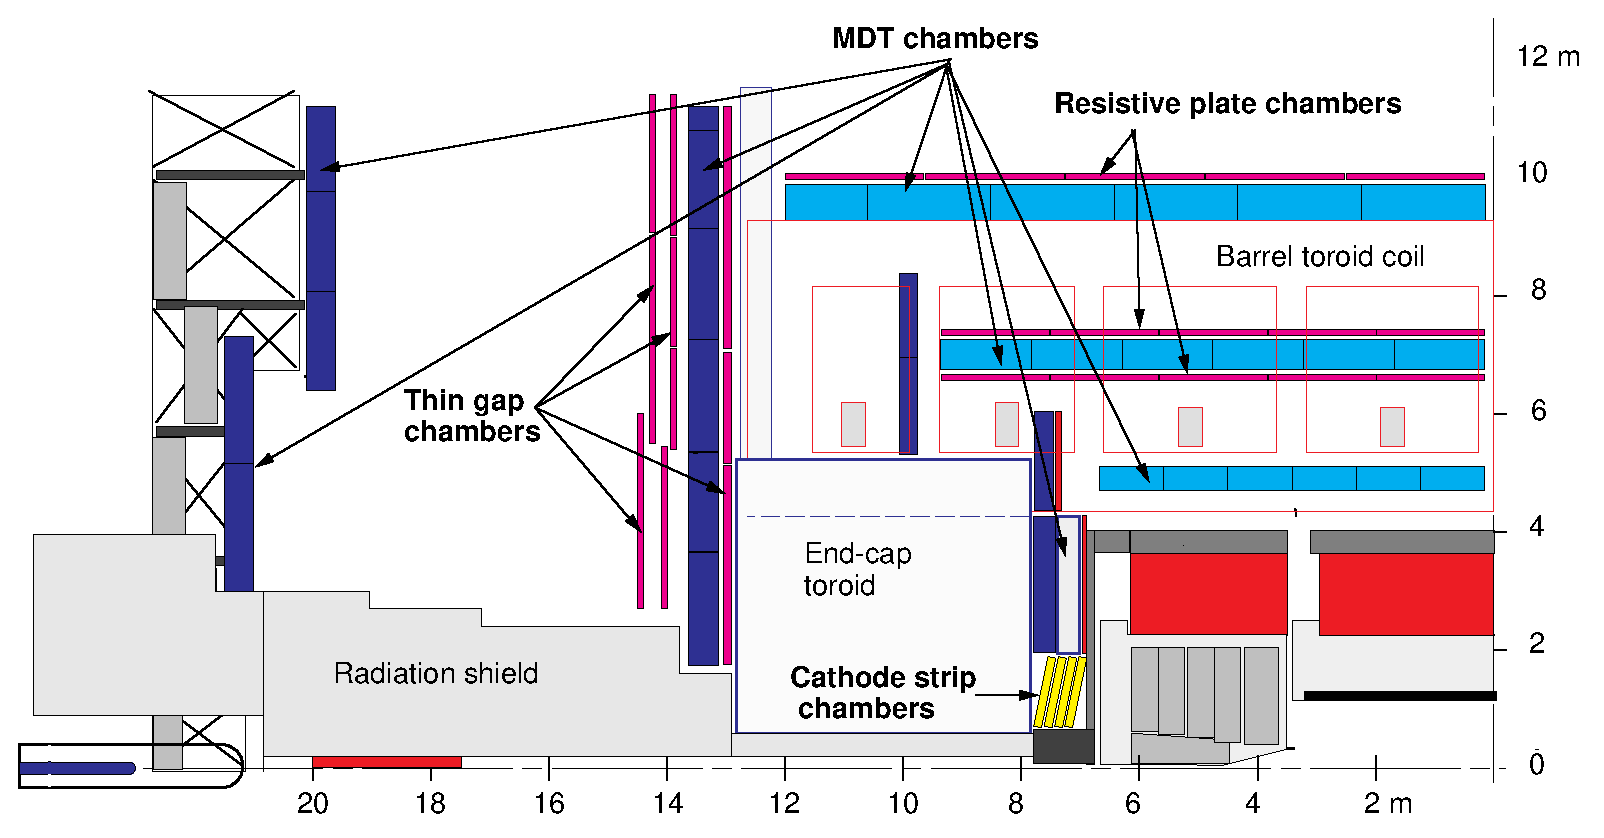
\includegraphics[width=.45\textwidth,keepaspectratio=true]{chapters/chapter3_experiment/images/ATLAS-muon-rz-tdr.eps}} \\
		% \subfloat[\label{fig:muon-spec_c}]{\includegraphics[width=.45\textwidth,keepaspectratio=true]{chapters/chapter3_experiment/images/ATLAS-muon-xy-tdr.eps}}
		% \caption{\label{fig:muon-spec} (a)   (b)}
		% \end{figure}

		\begin{figure}[!ht]
		\centering
		\includegraphics[width=\textwidth,keepaspectratio=true]{chapters/chapter3_experiment/images/ATLAS_Muon_System_Run3.png}
		\caption{Cut-out view of the \gls{ATLAS} detector Muon Spectrometer. \textcolor{red}{REFERENCE WAITING FOR PAPER TO BECOME PUBLIC}}
		\label{fig:muon-spec}
		\end{figure}

	\subsection{Trigger System}\label{ssec:trigger}
		The large luminosity provided by the \gls{LHC} is critical in collecting enough data to make detailed physics analyses. However, it also means that there is an incredibly large amount of data to sort through. So much that it is not possible to write out the data from every bunch crossing. As shown in Figure \ref{fig:high-pileup-event-display}, even one single event can contain an inordinate amount of data. Another issue arises due to the nature of hadron collisions; in that not all bunch crossing provide hard scatter inelastic collisions that are ``interesting'' enough to save data on. 

		To solve this issue, the data coming out of \gls{ATLAS} is combed through in real time at a variable rate of 1 kHz to 40 MHz. This is done with a \gls{TDAQ} system. The \gls{TDAQ} system used in Run-2 is described in detail here: \cite{ATLAS-trigger-Run2}. The \gls{TDAQ} system reads in data from the \gls{ATLAS} detector, calculates relevant quantities, and makes a decision on if there was an event worth storing. A diagram showing the data flow into the \gls{TDAQ} system is show in \ref{fig:trigger-run2}.\footnote{Figure \ref{fig:trigger-run2} shows the Fast TracKer (FTK). During Run 2 FTK was undergoing commissioning and was not used in the active \gls{TDAQ} system.} 
		\begin{figure}[!ht]
		\centering
		\includegraphics[width=\textwidth,keepaspectratio=true]{chapters/chapter3_experiment/images/Trigger_Run2.png}
		\caption{The \gls{ATLAS} \gls{TDAQ} system in Run-2 showing the components relevant for triggering as well as the detector read-out and data flow. \textcolor{red}{REFERENCE WAITING FOR PAPER TO BECOME PUBLIC}}
		\label{fig:trigger-run2}
		\end{figure}
		The \gls{ATLAS} \gls{TDAQ} system consists of two main components, \gls{L1} and \gls{HLT}. The \gls{L1} is a hardware based trigger system that reads in data from the calorimeters and muon spectrometer. The \gls{L1} has a latency of $2.5 \, \mu \mathrm{s}$ and can read-out accepted events up to 100 kHz, the detector maximum readout rate. The \gls{HLT} is a software based trigger system based on the offline reconstruction software. During Run-2 the \gls{HLT} operated with an average output rate of 1.2 kHz, which translates to about 1.2 GB/s of data sent to permanent storage.	

		After the \gls{TDAQ} system accepts an event, the data is set to be stored on magnetic tape for long term storage. It is also processed at the local computing farm named Tier-0 with the full reconstruction software suite described in Chapter \ref{chap:reco}.


\chapter{Simulation}\label{chap:sim}
	The data collected by the ATLAS experiment must be compared to a control. This control is most often a dataset of simulation particle collisions that approximate to great precision physics processes and particle interaction with detector material, as well as the detector's response. Figure \ref{fig:simulation} shows the chain of simulations these datasets are produced by. 
	\begin{figure}[!ht]
	\centering
	\includegraphics[width=.95\textwidth,keepaspectratio=true]{chapters/chapter4_simulation/images/Simulation_Chain.png}
	\caption{\label{fig:simulation} A pictorial representation of the simulation chain used in the ATLAS experiment. \cite{Wanotayaroj:2242196}}
	\end{figure}
	
	Many particle physics experiments, ATLAS included, use Monte Carlo (MC) simulation techniques to produce these datasets. Monte Carlo simulation techniques use repeated random sampling of underlying probability density functions to closely model various processes. 

	\section{Event Generation and Hadronization}\label{sec:event-gen}
	Since protons and other hadrons are not fundamental particles, it is impossible to know the exact constituents (partons) that interacted during a collision. To mimic this intrinsic probabilistic nature, Parton Distribution Functions (PDFs) are used. Where a PDF models the probability of any parton within a proton (or hadron) to carry a fraction of the beam energy as momentum. The PDF and subsequent inelastic hard scattering of the interacting partons are modeled via a Matrix Element (ME) calculation, often depicted through Feynman diagrams. This ME calculation is done to fixed order in perturbation theory, leading order (LO), next-to-leading order (NLO), leading-logarithmic order (LL), etc. This first level event generation can be done by a myriad of MC event generators. Often specific choices are made based on individual generator performance for a given physics process.

	The next step in the simulation chain is the parton showering or hadronization. This is often done with a completely different set of MC generators. Hadronization is a complex, computationally expensive step to simulate and is done through iteratively. An example of a parton shower generator output can be seen in figure \ref{fig:hadronization}.

	\begin{figure}[!ht]
	\centering
	\includegraphics[width=\textwidth,keepaspectratio=true]{chapters/chapter4_simulation/images/tth_hadronization_gen.png}
	\caption{\label{fig:hadronization} A pictorial representation of a parton shower of a t$\bar{\mathrm{t}}$H event. \cite{Wanotayaroj:2242196}}
	\end{figure}	

	\section{Detector Simulation}\label{sec:detector-sim}
	The final step in the simulation chain is simulating the particle's interaction with the detector material and the detector's response. Up until this point, the MC generators used are generic non-experiment dependent simulations. The ATLAS collaboration uses a GEANT4 based generator suite to simulate these interactions. \cite{GEANT4} These simulations are incredibly detailed, including all support structure, material densities, readout electronics, digitization, etc. The final simulated dataset is output into a raw data format identical to real data coming off of the ATLAS detector.
\chapter{Event Reconstruction}\label{chap:reco}
	Before any physics analysis can be performed on the raw data from the ATLAS detector and MC simulations both raw datasets go through a reconstruction software suite called Athena. Various algorithms are employed to identify energy deposits as particles based on shower shapes, track hits, calculated charge to mass ratios, etc. The following sections detail the identification processes of muons, electrons, photons, jets, $\tau$ leptons, and a calculated quantity called missing transverse energy $(\Etm)$.

	\section{Muon Identification}\label{sec:reco-muon}

	\section{e $\gamma$ Identification}\label{sec:reco-egamma}

	\section{Jet Clustering}\label{sec:reco-jets}

		\subsection{\bjet Tagging}\label{ssec:flavor-tagging}

	\section{$\tau$ Identification}\label{ssec:reco-tau}

	\section{\Etm}\label{sec:reco-etmiss}
		
\chapter{Search for Charged Higgs Bosons}\label{chap:hpana}
	This chapter details a search for a charged Higgs boson decaying to a hadronically decaying tau lepton and a neutrino; the phenomenology is discussed in Section \ref{sec:Hpm}. The search contains two subchannels, \taujets and \taulep based on the decay of the associated top quark in the collision event. The \taujets subchannel ($t\to Wb, \, W \to q\bar{q}$)  has a higher branching fraction, leading to higher sensitivity at larger \mHpm values. The \taulep subchannel ($t\to Wb, \, W \to \ell \nu$)  has a much lower branching fraction, but takes advantage of single-lepton triggers which enhance background suppression of \acrshort{QCD} $\mathrm{jet} \, \to \, \tau$ fakes. This leads to an increased sensitivity at lower \mHpm values. The extra neutrino in the \taulep decay mode creates extra difficulties in separating signal from background in this subchannel by adding a significant contribution to the \Etm calculation for the event. 

	The search described by this dissertation uses a profile likelihood ratio as the test statistic in a simultaneous fit in two \glspl{CR} and three \glspl{SR}. The discriminating variable is chosen to be the output score distribution of a \gls{MVA}. In the previous publication described in Section \ref{ssec:Prev Hpm} several \gls{BDT} were used, binned in \mHpm; this analysis uses a \gls{PNN} to classify events as signal-like or background-like.

	This chapter discusses in detail the entire analysis, including the signal signatures, event selections, analyzed datasets, modeling of backgrounds, training and evaluation of classifiers, studies of systematic uncertainties, and results.

	\section{Signature and Event Selection}\label{sec:signal}
		As shown in Figure \ref{fig:hpm-diagrams}, the production of the \Hpm is dependent on its mass \mHpm. Table \ref{tab:hplus-production} shows the production mechanisms for \mHpm values in bins of the top quark mass $m_t$ as well as the main decay mode (and theoretical constraints), and the main source of background. Three mass ranges are defined, low mass $80 \leq \mHpm \leq 130 $ GeV, intermediate mass $140 \leq \mHpm \leq 190$, and high mass $200 \leq \mHpm \leq 3000$ GeV. In the low mass bin the \Hpm takes the place of the $W^{\pm}$ in the top quark decay. Results of searches for other non-standard decays of top quarks limits on the branching ratio can be seen in Reference \cite{pdg}. The two subchannels of this analysis have similar signal signatures with a hard-scatter source of \Etm, one \tauhad, and at least 1 \bjet from the associated top decay. In the \taulep subchannel there is an extra requirement of a lepton (e or $\mu$). Due to the variable amount of energy available to the final state products based on \mHpm the event topology changes as a function of \mHpm. As described in Section \ref{sec:mva}, classifiers are trained and evaluated in \mHpm bins to account for the varying event topology.

		\begin{table}[!thp]
			\centering
			\resizebox{\textwidth}{!}{
			\begin{tabular}{| c | c | c | c |}
			\hline
			\textbf{\Hpm Mass} & \textbf{Production Mechanism} & \textbf{Decay}  & \textbf{Main Backgrounds}\\
			\hline \hline
			\multicolumn{1}{|c|}{\multirow{2}{*}{$\mHpm < m_{t}$}} 		& \begin{tabular}[c]{@{}c@{}} double-resonant $t \to H^\pm b$ (LO) \\ \includegraphics[width=.19\textwidth]{chapters/chapter6_HPlus/images/double_resonant_production_low_mass.png} \end{tabular} 											& \begin{tabular}[c]{@{}c@{}} \HpmLong \\ (low $\tanb \implies$ $\Hpm \to cs$ or $\Hpm \to cb$ ) \end{tabular} 																	& \ttbar, single-top \\ \hline

			\multicolumn{1}{|c|}{\multirow{3}{*}{$\mHpm \simeq m_{t}$}} & \begin{tabular}[c]{@{}c@{}} non-resonant $t \to \Hpm b$ (LO) \\ \includegraphics[width=.19\textwidth]{chapters/chapter6_HPlus/images/non_resonant_production_intermediate_mass.png} \\ interferences taken into account \end{tabular} 	& $\Hpm \to \tau \nu$  																																									& \ttbar, single-top \\ \hline

			\multicolumn{1}{|c|}{\multirow{3}{*}{$\mHpm > m_{t}$}}		& \begin{tabular}[c]{@{}c@{}} single-resonant $gg \to tbH^\pm$ (NLO) \\ \includegraphics[width=.19\textwidth]{chapters/chapter6_HPlus/images/single_resonant_production_large_mass.png} \end{tabular} 										& \begin{tabular}[c]{@{}c@{}} $\Hpm \to tb$ \\ ($cos(\beta-\alpha) \simeq 0$ and large $tan(\beta) \implies \Hpm \to \tau \nu$ \\ $BR(\HpmLong) \simeq 10-15\%$ ) \end{tabular} & multi-jet \\ \hline

			\end{tabular}}
			\caption{\Hpm production mechanisms based on \mHpm, dominant \Hpm decay mode, and the main backgrounds associated with the diagram.}
			\label{tab:hplus-production}
		\end{table}

		\subsection{Object Definitions}\label{ssec:object-def}
			After physics objects are reconstructed additional kinematic and identification cuts are applied to allow for high identification efficiency while keeping significant statistics \cites{tau-id-rnn}{jet-calibration}{b-tagging}{electron-perf}{muon-id}. Table \ref{tab:object-defs} shows the identification requirements on all objects used in the analysis. In both subchannels \tauhad candidates are required to fit the medium working point described in Section \ref{ssec:reco-tau} that corresponds to a 75\% efficiency for 1-prong and 60\% efficiency for 3-prong \tauhad identification, an $\abs{\eta}$ cut of $< 2.3$ that also excludes the gap and crack region of the ATLAS calorimeters at $1.37 < \abs{\eta} < 1.52$, and an overlap removal with electrons. For the \taujets subchannel, the \tauhad \pt is required to be greater than 40 GeV and greater than 30 GeV for the \taulep subchannel. Although muons and electrons are not part of the \taujets signal final state, a loose identification and isolation requirement is used to veto events; while the \taulep subchannel requires there to be either an electron or a muon that passes the tight identification and isolation requirements as well as a \pt above 30 GeV. The jets in candidate events are required to have greater than 25 GeV in \pt and are made with the anti-$k_t$ algorithm with R=0.4. Any event that contains a jet with $\pt > 25$ GeV and fails quality cuts is discarded. This ensures that no jet is consistent with having originated from instrumental effects or non-collision backgrounds. Jets tagged as \bjets are done so at a 70\% efficient working point using the DL1r tagger described in Section \ref{ssec:flavor-tagging}. The \pt requirements listed above for each physics object were chosen to maximize identification efficiency of each object. An example of identification efficiency can be seen for electrons in Figure \ref{fig:electron-efficiency}. The chosen cut of $\pt^{e}>30$ GeV corresponds to an identification efficiency of $\approx 70\%$. Similar choices for $\tau$ leptons \cite{tau-id-rnn}, jets \cite{jet-calibration}, \bjets \cite{b-tagging}, \Etm \cite{met-perf}, and muons \cite{muon-calibration} were made. 

			\begin{table}[!thp]
				\centering
				\resizebox{\textwidth}{!}{
				\begin{tabular}{| c | l | l |}
				\hline
				Object & \textbf{\taujets} & \textbf{\taulep} \\
				\hline \hline
				\multicolumn{1}{|c|}{\multirow{3}{*}{\tauhad}} & \begin{tabular}[c]{@{}c@{}}Leading reconstructed $\tau$ (regardless of its ID), \\ mediumID$^{*}$, $\pt > 40$ GeV, $\abs{\eta}^{***} < 2.3$, $e$ OLR \end{tabular} & \begin{tabular}[c]{@{}c@{}} Leading reconstructed $\tau$ (regardless of its ID), \\ mediumID$^{*}$, $\pt > 30$ GeV, $\abs{\eta}^{***} < 2.3$, $e$ OLR \end{tabular} \\[4ex] \hline
				\multicolumn{1}{|c|}{\multirow{3}{*}{$e$}} & \begin{tabular}[c]{@{}c@{}} LoseLLH, $\pt > 20$ GeV, $\abs{\eta}^{***} < 2.47$, \\ Loose isolation, IP cuts \end{tabular} &  \begin{tabular}[c]{@{}c@{}} TightLLH, $\pt > 30$ GeV, $\abs{\eta}^{***} < 2.47$, \\ Tight isolation, IP cuts \end{tabular} \\[4ex] \hline
				\multicolumn{1}{|c|}{\multirow{3}{*}{$\mu$}} & \begin{tabular}[c]{@{}c@{}} LooseID, $\pt > 20$ GeV, $\abs{\eta} < 2.5$, \\Loose isolation, IP cuts \end{tabular} & \begin{tabular}[c]{@{}c@{}} TightID, $\pt > 30$ GeV, $\abs{\eta} < 2.5$,\\ Tight isolation, IP cuts \end{tabular} \\[4ex] \hline 
				\multicolumn{1}{|c|}{\multirow{3}{*}{jet}} & \begin{tabular}[c]{@{}c@{}} AntiKt4EMPFlow, $\pt > 25$, GeV $\abs{\eta} < 2.5$,\\ JVT$^{**}$  $> 0.59$, Btag=70\%, DL1r \end{tabular} & \begin{tabular}[c]{@{}c@{}} AntiKt4EMPFlow, $\pt > 25$ GeV, $\abs{\eta} <2.5$, \\ JVT$^{**}$  $ > 0.59$ , Btag=70\%, DL1r \end{tabular} \\[4ex] \hline
				\end{tabular}}
				\caption{Definitions of physics objects used in this analysis.}
				\label{tab:object-defs}
			\end{table}

			\begin{figure}
			\begin{center}
			\includegraphics[width=\textwidth,keepaspectratio=true]{chapters/chapter6_HPlus/images/Electron_ID_Efficiency.png}
			\end{center}
			\caption{The electron identification efficiency in $Z\to ee$ events in data as a function of $E_{T}$ for the Loose, Medium, and Tight operating points. The efficiencies are obtained by applying data-to-simulation efficiency ratios measured in $J/\Psi \to ee$ and $Z \to ee$ events to $Z \to ee$ simulation. The inner uncertainties are statistical and the total uncertainties are the statistical and systematic uncertainties in the data-to-simulation efficiency ratio added in quadrature. The bottom panel shows the data-to-simulation ratio. Taken from Reference \cite{electron-perf}. }
			\label{fig:electron-efficiency}
			\end{figure}

			% \begin{columns}
			% \column{.3\textwidth}
			% \begin{itemize}
			%   \footnotesize
			%   \item $\tau$ mediumID$^{*}$
			%   \begin{itemize}
			%     \tiny
			%     \item 1-prong: 75\% ID eff 
			%     \item 3-prong: 60\% ID eff
			%   \end{itemize}
			% \end{itemize}
			% \column{.3\textwidth}
			% \begin{itemize}
			%   \footnotesize
			%   \item JVT$^{**}$
			%     \begin{itemize}
			%       \tiny
			%       \item $\pt < 60$ GeV
			%       \item $\abs{\eta}<2.4$
			%   \end{itemize}
			% \end{itemize}
			% \column{.3\textwidth}
			% \begin{itemize}
			%   \footnotesize
			%   \item $\abs{\eta}^{***}$
			%     \begin{itemize}
			%       \tiny
			%       \item $1.37 < \abs{eta} < 1.52 $ excluded
			%   \end{itemize}
			% \end{itemize}
			% \end{columns}

		\subsection{Event Selections}\label{ssec:event-selection}
			Each subchannel signal region has stricter requirements than the object definitions described in Section \ref{ssec:object-def}. Table \ref{tab:signal-regions} details these selections. The channels differ in the triggers used; the \taujets subchannel relies on \Etm triggers while the \taulep subchannel relies on single lepton triggers. Detailed information on the triggers and the efficiencies of the trigger options can be found in References \cite{MET-Trigger} (\Etm), \cite{Electron-Trigger} ($e$), and \cite{Muon-Trigger} ($\mu$).  Due to the difficulty of separating signal from background and the large amount of background, the \taujets subchannel has a higher \pt cut on the \tauhad of $40$ GeV as opposed to the \taulep value of $30$ GeV. In addition, a higher value of \Etm of $150$ GeV is required for the \taujets subchannel compared to $50$ GeV in the \taulep subchannel. In the \taujets subchannel a value of $50$ GeV is also required of the transverse mass $m_{T}$ defined as 
			\begin{equation}\label{eqn:transverse-mass}
			m_{T} = \sqrt{ 2 \pt^{\tau} \Etm (1 - cos \Delta \phi_{\tau,\Etm}) }
			\end{equation}
			The \taulep has no such requirement, but does require the \tauhad and lepton to have opposite electromagnetic charge. A set of orthogonal \glspl{CR} are defined for each subchannel to verify proper background modelling and are described in Section \ref{sec:bkg-modeling}. The acceptance of signal in the signal regions defined in Table \ref{tab:signal-regions} is shown in Figure \ref{fig:signal-acceptance}. The instability of the data points is due to the boundaries of the \Hpm production diagrams.  Due to the larger branching fraction of $t \to W+b;  W \to q\bar{q}$ as opposed to $t \to W+b; W \to \ell + \nu$ the \taujets subchannel has a factor of 10 larger signal acceptance than the \taulep subchannel. In both channels, the signal acceptance decreases for \mHpm values $> 1000$ GeV. This is an artifact of objects becoming boosted, meaning their decay products are extremely collimated, resulting in lower efficiencies for object identification.

			\begin{table}[!thp]
				\centering
				\resizebox{.75\textwidth}{!}{
				\begin{tabular}{| c | c |}
				\hline
				\textbf{$\tau + jets$ SR } & \textbf{$\tau + \ell$ SR} \\
				\hline \hline
				$\Etm$ Trigger  																& Single lepton triggers (e or $\mu$) \\[1.2ex] \hline
				1 \tauhad ; $\pt^{\tau} > 40$ GeV 							& 1 \tauhad ; $\pt^{\tau} > 30$ GeV\\[1.2ex] \hline
				0 $\ell$ (e or $\mu$) ; $\pt^{\ell} > 20$ GeV  	& 1 $\ell$ (e or $\mu$) ; $\pt^{\ell} > 30$ GeV \\[1.2ex] \hline
				$\geq$ 3 jets ; $\pt^{j} > 25$ GeV  						& $\geq$ 1 jet ; $\pt^{j} > 25$ GeV \\[1.2ex] \hline
				$\geq$ 1 \bjets ; $\pt^{\bjet} > 25$ GeV 				& $\geq$ 1 \bjets ; $\pt^{\bjet} > 25$ GeV \\[1.2ex] \hline
				\Etm$ > 150$ GeV 																& \Etm$ > 50$ GeV \\[1.2ex] \hline
				$m_{T}(\tau,\Etm) > 50$ GeV 										& Opposite sign $\tau$ and $\ell$ \\[1.2ex] 
				\hline
				\end{tabular}}
				\caption{\taujets and \taulep signal region definitions.}
				\label{tab:signal-regions}
			\end{table}

			\begin{figure}[!ht]
				\centering
				\subfloat[\label{fig:signal-acceptance_a}]{\includegraphics[width=0.5\textwidth]{chapters/chapter6_HPlus/images/Signal_Acceptance_Efficiency_SR_TAUJET.pdf}}
				\subfloat[\label{fig:signal-acceptance_b}]{\includegraphics[width=0.5\textwidth]{chapters/chapter6_HPlus/images/Signal_Acceptance_Efficiency_SR_TAULEP.pdf}}
				\caption{\label{fig:signal-acceptance} Signal acceptance as a function of the charged Higgs boson mass for both the \taujets (a) and \taulep subchannels (b). Statistical errors are shown but are negligible.}
			\end{figure}

	\section{Datasets}\label{sec:datasets}
		This analysis uses the full Run-2 ATLAS dataset collected between 2015 and 2018 corresponding to $139.0 \pm 2.4$ \ifb \cite{lumi-run2}. The datasets used are required to be included in the ATLAS ``Good Run Lists'' (GRLs), meaning they have passed nominal data quality checks with all detector subsystems operating within normal conditions. Further event cleaning is applied that removes events in which a reconstructed jet originated from detector noise or non-collision backgrounds. The collection of data throughout Run-2 can be seen in Figure \ref{fig:lhc-lumi}.

		\subsection{Signal Modeling}\label{ssec:sig-modeling}
		\gls{MC} simulations of \Hpm signal events are generated at varying orders dependent on \mHpm. In all cases, the 2HDM Type II model described in Section \ref{ssec:2HDM} is assumed and the generator MadGraph is used. The lower mass range corresponding to $\mHpm < 140$ GeV where a \Hpm takes the place of a $W^{\pm}$ in a top decay is generated at LO. The intermediate mass range of $140 \leq \mHpm < 200 $ GeV is generated at LO, taking into account the non-resonant, single-top resonant and double-resonant diagrams and their interferences. In this mass range, the final state contains one \Hpm, one $W^{\pm}$, and two b quark. For charged Higgs masses of 200 GeV and above, the \Hpm is produced in association with a top quark and is generated at NLO. The Powheg-box v2 \cites{powheg-1}{powheg-2} generator is used with the NNPDF3.0 \gls{NLO} \gls{PDF} \cite{PDFs-2} set in the matrix element calculations to generate \ttbar and single top-quarks in the W t- and s-channels. In all cases, the parton generator is interfaced with Pythia v8.230 \cite{pythia} with the NNPDF2.3 \gls{LO} \gls{PDF} \cite{PDFs-1} using the A14 underlying event tuning parameters \cite{Pythia8-tunes}. Table \ref{tab:signal-generated} shows the cross section and raw number of events generated for each \mHpm point for both subchannels.

		\begin{table}[!thp]
			\centering
			\resizebox{.65\textwidth}{!}{
			\begin{tabular}{| l | l | l | l |}
			\hline
			\mHpm [GeV] 	& $\sigma$ [pb] 	& \taulep Generated Events 	& \taujets Generated Events 	\\ \hline
			80 				& 61.639 			& 220k 						& 110k							\\
			90 				& 52.823 			& 220k 						& 110k							\\
			100 			& 43.777 			& 220k 						& 110k							\\
			110				& 34.770 			& 220k 						& 110k							\\
			120 			& 26.092 			& 220k 						& 110k							\\
			130 			& 18.069 			& 220k 						& 110k							\\ \hline
			140 			& 15.023 			& 220k 						& 220k							\\
			150 			& 7.681 			& 220k 						& 220k							\\
			160 			& 2.665 			& 220k 						& 220k							\\
			170 			& 0.63748 			& 220k 						& 220k							\\
			180 			& 0.52979 			& 220k 						& 220k							\\
			190 			& 0.47201 			& 220k 						& 220k							\\ \hline
			200 			& 0.55632 			& 110k 						& 220k							\\
			225 			& 0.44081 			& 110k 						& 220k							\\
			250 			& 0.3573 				& 110k 						& 220k							\\
			275 			& 0.28592 			& 110k 						& 220k							\\
			300 			& 0.23373 			& 110k 						& 220k							\\
			350 			& 0.15774 			& 110k 						& 220k							\\
			400 			& 0.10818 			& 110k 						& 220k							\\
			500 			& 0.054139 			& 110k 						& 220k							\\
			600 			& 0.02847 			& 110k 						& 220k							\\
			700 			& 0.015764 			& 110k 						& 220k							\\
			800 			& 0.009067 			& 110k 						& 220k							\\
			900 			& 0.005324 			& 110k 						& 220k							\\
			1000 			& 0.003271 			& 110k 						& 220k							\\
			1200 			& 0.001311 			& 110k 						& 220k							\\
			1400 			& 0.000558 			& 110k 						& 220k							\\
			1600 			& 0.000252 			& 110k 						& 220k							\\
			1800 			& 0.000120 			& 110k 						& 220k							\\
			2000 			& 0.0000587 		& 110k 						& 220k							\\
			2500 			& 0.0000111			& 110k 						& 220k							\\
			3000 			& 0.00000234		& 110k 						& 220k							\\ \hline
			\end{tabular}}
			\caption{For each \Hpm mass the generator xcross-section $(\sigma \times BR(\HpmLong))$ is given, as well as the number of generated events for both \taulep and \taujets subchannels.}
			\label{tab:signal-generated}
		\end{table}
		% \pagebreak

	\section{Background Modeling}\label{sec:bkg-modeling}
		The main sources of backgrounds are shown in Table \ref{tab:backgrounds}, separated between backgrounds with a prompt \tauhad in the hard scatter process and those that arise from the misidentification of other physics objects as a \tauhad. The cross section of all simulated background samples and the relevant generators can be seen in Table \ref{tab:bkg-xs}. Control regions that are designed to be orthogonal to the signal region are created for both subchannels in order to study the modeling of the backgrounds. These control regions are defined by the cuts in Table \ref{tab:taujet-control-regions} (\taujets) and Table \ref{tab:taulep-control-regions} (\taulep). For the \taulep subchannel the Same Sign and b-veto control regions are further split into two control regions, one that requires a $\mu$ in the event and another that requires an electron. 

		

    \begin{table}[!thp]
      \centering
      \resizebox{\textwidth}{!}{
      \begin{tabular}{| l | l |}
      \hline
      Backgrounds w/ prompt \tauhad & Backgrounds w/ fake $\tau$ \\
      \hline \hline
      $t\bar{t}$ estimated with \gls{MC}       & Fake $j \to \tau$ estimated with data driven fake factor method \\ \hline
      $W(Z)+jets$ estimated with \gls{MC}         & Fake $\ell \to \tau$ estimated with \gls{MC}, validated on $Z \to ee$\\ \hline
      Diboson estimated with \gls{MC} & \\
      \hline
      \end{tabular}}
      \caption{Dominant backgrounds from prompt \tauhad and fake \tauhad candidates.}
      \label{tab:backgrounds}
    \end{table}

		\begin{table}[!thp]
			\begin{center}
			\small
			\resizebox{0.5\textwidth}{!}{
			\begin{tabular}{|c||c|c|}
			\hline
			Background process & Generator \& & Cross section \\
			  & parton shower & number(s) [pb] \\
			\hline \hline
			$\begin{array}{c}
			$\ttbar$~\mbox{with at least one lepton $\ell$} \\ 
			\end{array}$ &
			$\begin{array}{c}
			\mbox{{\textsc Powheg}}~\& \\
			\mbox{{\textsc Pythia8}}
			\end{array}$
			& 729.77* \\
			\hline
			$\begin{array}{c}
			\mbox{Single top-quark}\\ 
			\mbox{$t$-channel}
			\end{array}$ & & 59.17* \\
			$\begin{array}{c}
			\mbox{Single top-quark}\\ 
			\mbox{$s$-channel}
			\end{array}$ &
			$\begin{array}{c}
			\mbox{{\textsc Powheg}}~\& \\
			\mbox{{\textsc Pythia8}}
			\end{array}$ & 3.29* \\
			$\begin{array}{c}
			\mbox{Single top-quark}\\ 
			\mbox{$Wt$-channel}
			\end{array}$  & & 83.83  \\
			\hline
			$\begin{array}{c}
			~ \\
			W(\ell\nu) + \mbox{jets} \\ 
			~ \\
			\end{array}$ &
			$\begin{array}{c}
			~ \\
			\mbox{Sherpa 2.2.1} \\ 
			~ \\
			\end{array}$ &
			$\begin{array}{c}
			2.0\times 10^4 \\
			2.0\times 10^4 \\ 
			2.0\times 10^4 \\
			\end{array}$ \\
			\hline
			$\begin{array}{c}
			Z/\gamma^{\ast}(\ell\ell,\nu\nu) + \mbox{jets} \\
			\end{array}$ & 
			$\begin{array}{c}
			~ \\
			\mbox{Sherpa 2.2.1} \\ 
			~ \\
			\end{array}$  &
			$\begin{array}{c}
			2.1 \times 10^3  \\
			2.1 \times 10^3  \\ 
			2.1 \times 10^3  \\
			\end{array}$ \\

			\hline
			$WW$  &  & 54.81 \\
			$WZ$  &  $\begin{array}{c}
			\mbox{{\textsc Powheg}}~\& \\
			\mbox{{\textsc Pythia8}}
			\end{array}$ & 16.34 \\
			$ZZ$  &  & 8.94 \\
			\hline
			\end{tabular}}
			\normalsize
			\caption{\label{tab:bkg-xs}
			Cross sections for the main \acrshort{SM} 
			background samples at \sqs. 
			Here, $\ell$ refers to the three lepton families $e$, $\mu$ and 
			$\tau$. All background cross sections are normalized to NNLO predictions, 
			except for diboson events, where the NLO prediction is used. A '*' indicates
			that the quoted cross section for the sample is neglecting leptonic/hadronic
			branching ratios.
			}
			\end{center}
		\end{table}

		% \begin{table}[!thp]
		% 	\begin{subtable}[c]{0.45\textwidth}
		% 		\centering
		% 		\begin{tabular}{| c |}
		% 			\hline
  %       	\textbf{\ttbar Control Region} \\ \hline \hline
  %         1 \tauhad \\
  %         $\pt^{\tau} > 40 $ GeV \\
  %         $\geq 3 $ jets\\
  %         $\geq 2 $ \bjets\\
  %         $\Etm > 150 GeV$ \\
  %         $m_{T}(\tau, \Etm) < 100 \: GeV$ \\
  %         \hline
		% 		\end{tabular}
		% 		\subcaption{\ttbar modeling}
		% 	\end{subtable}
		% 	\begin{subtable}[c]{.45\textwidth}
		% 		\centering
		% 		\begin{tabular}{| c |}
		% 			\hline
		% 			\textbf{b-veto Control Region} \\ \hline \hline
		% 			1 \tauhad \\
		% 			$\pt^{\tau} > 40 \: GeV $  \\
		% 			$\geq 3$ jets\\
		% 			% $n\_bjets > 2$ \\
		% 			$\pt^{jet} > 25 \: GeV$ \\
		% 			$\Etm > 150 GeV$ \\
		% 			$m_{T}(\tau, \Etm) > 50 \: GeV$ \\
		% 			b veto \\
		% 			$\ell$ veto \\
		% 			\hline
		% 		\end{tabular}
		% 		\subcaption{Close to signal region}
		% 	\end{subtable}
		% 	\begin{subtable}[c]{.45\textwidth}
		% 		\centering
		% 		\begin{tabular}{| c |}
		% 			\hline
		% 			\textbf{W+Jets Control Region} \\ \hline \hline
		% 			1 \tauhad \\
		% 			$\pt^{\tau} > 40 \: GeV $  \\
		% 			$\geq 3$ jets \\
		% 			$\pt^{jet} > 25 \: GeV$ \\
		% 			$\Etm > 150 GeV$ \\
		% 			$m_{T}(\tau, \Etm) > 100 \: GeV$ \\ 
		% 			b veto \\
		% 			$\ell$ veto \\
		% 			\hline
		% 		\end{tabular}
		% 		\subcaption{W+Jets modeling}
		% 	\end{subtable}
		% 	\begin{subtable}[c]{.45\textwidth}
		% 		\centering
		% 		\begin{tabular}{| c |}
		% 			\hline
		% 			\textbf{b-veto $m_{T}\geq100$ Control Region} \\ \hline \hline
		% 			1 \tauhad \\
		% 			$\pt^{\tau} > 40 \: GeV $  \\
		% 			$\geq 3$ jets \\
		% 			$\pt^{jet} > 25 \: GeV$ \\
		% 			$\Etm > 150 GeV$ \\
		% 			$m_{T}(\tau, \Etm) > 100 \: GeV$ \\
		% 			b veto \\
		% 			$\ell$ veto \\
		% 			\hline
		% 		\end{tabular}
		% 		\subcaption{Fake $j \to \tau$ enriched region}
		% 	\end{subtable}

		% 	\caption{Control region definitions for the \taujets subchannel.}
		% 	\label{tab:taujet-control-regions}
		% \end{table}

		% \begin{table}[!thp]
		% 	\begin{subtable}[c]{0.45\textwidth}
		% 		\centering
		% 		\begin{tabular}{| c |}
		% 			\hline
  %       	\textbf{Dilepton-btag CR} \\ \hline \hline
  %         $\tau$ veto \\
  %         $n\geq 1$ jets \\
  %         $\pt^{jet} > 25 GeV$ \\
  %         $\geq 1$ \bjets \\
  %         $\Etm > 50 GeV$ \\
  %         1 $e$ \\
  %         1 $\mu$ \\
  %         \hline
		% 		\end{tabular}
		% 		\subcaption{\ttbar and single top modeling}
		% 	\end{subtable}
		% 	\begin{subtable}[c]{.45\textwidth}
		% 		\centering
		% 		\begin{tabular}{| c |}
		% 			\hline
	 %        \textbf{b-veto CR} \\ \hline \hline
  %         1 \tauhad \\
  %         $\pt^{\tau} > 30 \: GeV $  \\
  %         1 $e (\mu) $ \\
  %         Veto $\mu \:(e)$ \\
  %         Opposite sign $\tau$ $e \: (\mu)$ \\
  %         $\geq 1$ jets  \\
  %         $\pt^{jet} > 25 GeV$ \\
  %         $\Etm > 50 GeV$ \\
  %         1 tight $e \: (\mu)$ \\
  %         \hline					
		% 		\end{tabular}
		% 		\subcaption{Close to signal region}
		% 	\end{subtable}
		% 	\begin{subtable}[c]{.45\textwidth}
		% 		\centering
		% 		\begin{tabular}{| c |}
		% 			\hline
  %       	\textbf{Zee CR} \\ \hline \hline
  %         1 \tauhad \\
  %         $\pt^{\tau} > 30 \: GeV $  \\
  %         veto $\mu$ \\
  %         Opposite sign $\tau$ $e$ \\
  %         $\geq 1$ jets \\
  %         $\pt^{jet} > 25 GeV$ \\
  %         \bjet veto \\
  %         $\Etm > 50 GeV$ \\
  %         1 $e$\\
  %         $40 < mass(\tau,e) < 140 GeV$ \\
  %         \hline
		% 		\end{tabular}
		% 		\subcaption{Fake $\ell \to \tau$ enriched region}
		% 	\end{subtable}
		% 	\begin{subtable}[c]{.45\textwidth}
		% 		\centering
		% 		\begin{tabular}{| c |}
		% 			\hline
	 %        \textbf{Same Sign CR} \\ \hline \hline
  %         1 \tauhad \\
  %         $\pt^{\tau} > 30 \: GeV $  \\
  %         Same sign $\tau \: e(\mu)$ \\
  %         Veto $\mu\:(e)$ \\
  %         $\geq 1 jets$ \\
  %         $\pt^{jet} > 25 GeV$ \\
  %         $\Etm > 50 GeV$  \\
  %         1 tight $e \: (\mu)$ \\
  %         \hline
		% 		\end{tabular}
		% 		\subcaption{Fake $j \to \tau$ enriched region}
		% 	\end{subtable}

		% 	\caption{Control region definitions for the \taulep subchannel.}
		% 	\label{tab:taulep-control-regions}
		% \end{table}

		\begin{table}[!thp]
			\begin{tabular}{| c | c | c | c | c |} \hline
														& \ttbar CR 		& W+Jets CR 		& b-veto CR 		& b-veto $m_{T} > 100$ CR 						 	\\ \hline
				Number of \tauhad 	& 1 						& 1 						& 0 						& 0 																		\\ \hline
				$\pt^{\tau}$ 				& $ > 40$ GeV 	& $ > 40$ GeV 	& $ > 40$ GeV 	& $ > 40$ GeV 													\\ \hline
				Number of jets 			& $\geq 3$ 			& $\geq 3$ 			& $\geq 3$ 			& $\geq 3$ 															\\ \hline
				$\pt^{jet}$ 				& $\geq 25$ GeV & $\geq 25$ GeV & $\geq 25$ GeV & $\geq 25$ GeV 												\\ \hline
				Number of \bjets		& $\geq 2$ 			& 0 						& 0 						& 0 																		\\ \hline
				Number of $\ell$ 		& 0 						& 0 						& 0 						& 0 																		\\ \hline
				\Etm 								& $> 150$ GeV 	& $> 150$ GeV 	& $> 150$ GeV 	& $> 150$ GeV 													\\ \hline
				$m_{T}(\tau, \Etm)$	& $< 100$ GeV 	& $< 100$ GeV 	& $> 50 GeV$ 		& $> 100$ GeV 													\\ \hline
				Type of modeling 		& \ttbar 				& W+Jets 				& Close to SR 	& Fake $j \to \tau$ enriched 						\\ \hline
			\end{tabular}
			\caption{Control region definitions for the \taujets subchannel.}
			\label{tab:taujet-control-regions}
		\end{table}


		\begin{table}[!thp]
			\begin{tabular}{| c | c | c | c | c |} \hline
																& Dilepton-btag CR 				& Zee CR 												& b-veto CR 					& Same Sign $(\tau,\ell)$ CR 						 							\\ \hline
				Number of \tauhad 			& 0 											& 1 														& 0 									& 0 																		\\ \hline
				$\pt^{\tau}$ 						& $ > 30$ GeV 						& $ > 30$ GeV 									& $ > 30$ GeV 				& $ > 30$ GeV 													\\ \hline
				Number of jets 					& $\geq 1$ 								& $\geq 1$ 											& $\geq 1$ 						& $\geq 1$ 															\\ \hline
				$\pt^{jet}$ 						& $\geq 25$ GeV 					& $\geq 25$ GeV 								& $\geq 25$ GeV 			& $\geq 25$ GeV 												\\ \hline
				Number of \bjets				& $\geq 1$ 								& 0 														& 0 									& $\geq 1$ 															\\ \hline
				Number of $\ell$ 				& 2 (1 $e$, 1 $\mu$)			& 1 $e$													& 1 tight $e$ ($\mu$)	& 1 tight $e$ ($\mu$)										\\ \hline
				\Etm 										& $> 50$ GeV 							& $> 50$ GeV 										& $> 50$ GeV 					& $> 50$ GeV 														\\ \hline
				$\mathrm{mass}(\tau,e)$	& N/A 										& $> 40$; $< 140$ GeV 					& N/A 								& N/A 																	\\ \hline
				Type of modeling 				& \ttbar and single-top 	& Fake $\ell \to \tau$ enriched	& Close to SR 				& Fake $j \to \tau$ enriched 						\\ \hline
			\end{tabular}
			\caption{Control region definitions for the \taulep subchannel.}
			\label{tab:taulep-control-regions}
		\end{table}



		As seen in Table \ref{tab:backgrounds} misidentified objects appearing as \tauhad candidates comprise a significant portion of the total background. Fakes arising from $\ell \to \tau$ misidentification are well modeled in \gls{MC} simulations and are reweighted with scale factors provided by the ATLAS $\tau$ combined performance group. The mass of the \tauhad electron system can be seen in Figure \ref{fig:zee-mass} as verification of fake $\ell \to \tau$ modeling. Fakes due to $j \to \tau$ misidentification have poorly misunderstood systematic uncertainties associated with the fake \tauhad object and limited statistics of simulated events. To combat this, a data driven method is used to extract a scaling constant referred to as a fake factor.

		\begin{figure}[!thp]
			\centering
			\includegraphics[width=.5\textwidth,keepaspectratio=true]{chapters/chapter6_HPlus/images/taulep/tau_0_lep_0_mass_ZEE.png}
			\caption{Mass of $\tau$ - e system in the Zee control region. All systematics except for \ttbar theory uncertainties are included.}
			\label{fig:zee-mass}
		\end{figure}

		In the \taulep final state a significant portion of $j \to \tau$ fakes come from misidentifying \tauhad candidates in W+jets events that contain a true $\ell$ in the W decay and have a misidentified jet as a \tauhad. Fakes of this manner also arise from \acrshort{QCD}-like multi-jet interactions. The \gls{FF} method used to estimate the amount of expected fake \tauhad objects that pass the \tauhad identification procedure is described in Section \ref{ssec:reco-tau}. This method applies weights, or fake factors, to a subset of "anti-\tauhad" objects that have failed the selection and identification criteria in the signal region. A control region is defined to be rich in anti-\tauhad objects, where the \tauhad candidates fail the loose $\tau$ working point but have a small, non-zero $\tau$ identification \gls{RNN} score. The \gls{FF} and number of events with misidentified \tauhad objects $(N^{\tau}_{fakes})$ are defined as:
		\begin{equation}\label{eqn:ff}\begin{split}
		FF = \frac{ N^{\tau-id} }{N^{anti-\tau-id}} \\
		N_{fakes}^{\tau} = N^{anti-\tau}_{fakes} \times FF
		\end{split}\end{equation}
		Both of these values are then corrected for \tauhad candidates matching a true hadronic $\tau$ at generator level:
		\begin{equation}\label{eqn:ff-corrected}\begin{split}
		N^{\tau-id} = N^{\tau-id}(Data) - N^{\tau-id}(MC) \\
		N^{anti-\tau}_{fakes} = N^{anti-\tau}(Data) - N^{anti-\tau}_{true} (MC)
		\end{split}\end{equation}
		Two \glspl{CR} are created, one to capture the multi-jet (MJ) fakes and the other to study the W+jets fakes. The MJ \gls{CR} uses the \taujets signal region definition with an additional b-veto and an $\Etm < 80$ GeV cut. The W+jets \gls{CR}\footnote{This W+jets \gls{CR} is not the one defined in Table \ref{tab:taujet-control-regions}. This is a new region used to extract the fake factors.} uses the \taulep signal region definition with a b-veto, no \Etm cut, and a cut on the transverse mass of the $\ell$-\Etm system of $60 < m_{T}(\ell, \Etm)<160$ GeV.
		The \gls{FF} in the signal region is defined as 
		\begin{equation}\label{eqn:ff-sig}
		FF_{sig} = \alpha_{MJ} \times FF_{MJ} + (1 - \alpha_{MJ}) \times FF_{W+jets}
		\end{equation}
		where $\alpha$ is taken from a template fit of the $\tau$-ID score distributions of the anti-$\tau$s using template shapes from the anti-$\tau$ distributions in the MJ and W+jets control regions. In the signal regions, the number of events containing fake-\tauhad candidates is defined as
		\begin{equation}\label{eqn:nfakethad}
			N_{fake-\tau} = FF_{sig} \times N_{anti-\tau} 
		\end{equation}
		Figure \ref{fig:FF_COM} shows \gls{FF} plotted in each control region for 1-prong and 3-prong \tauhad binned in $\pt{\tau}$; extracted $\alpha$ values and their fits can be seen in Appendix \ref{app:fake-factors}.
		\begin{figure}[h!]
		  \begin{center}
		    \includegraphics[width=0.45\textwidth]{chapters/chapter6_HPlus/images/FFs/FFs_COM_inclusive__taujet.png} \qquad
		    \includegraphics[width=0.45\textwidth]{chapters/chapter6_HPlus/images/FFs/FFs_COM_inclusive__taulep.png} 
		  \end{center}
		  \caption{
		Combined \gls{FF} for the \taujets b-veto $\mathrm{m_{T}}>$100 control region, \taujets signal region, $\tau$+electron(muon) with same-sign control region and the \taulep signal region. Error bars represent systematic uncertainties of the method. 
		}
		  \label{fig:FF_COM}
		\end{figure}


		To verify background modeling, the \Etm distributions in each of the control regions are plotted with final scale factors including fake factors in Figure \ref{fig:bkg-met-taujets} (\taujets) and Figures \ref{fig:bkg-met-taulep-1} - \ref{fig:bkg-met-taulep-2} (\taulep). Similar distributions of the $\tau$ \pt can be seen in Figure \ref{fig:bkg-tau-pt-taujets} (\taujets) and Figures \ref{fig:bkg-tau-pt-taulep-1} - \ref{fig:bkg-tau-pt-taulep-2}. These plots include a ratio of reconstructed data events and simulated \gls{MC} events bin by bin to ensure proper modeling across variable shapes. More background modeling plots can be seen in Appendix \ref{app:valid-plots}. Tables \ref{tab:expected_yields_taujets}, \ref{tab:expected_yields_taue} and \ref{tab:expected_yields_taumu} show the expected event yields and the effect of each selection cut on the background sources as well as selected \mHpm values of 110, 170, and 1000 GeV. At the time of writing, the analysis is still blinded so data yields are not known.

		\begin{figure}[!thp]
			\begin{center}    
			% \includegraphics[width=0.45\textwidth]{chapters/chapter6_HPlus/images/taujets/met_et_TAUJET_PRESEL.png} \\
			\includegraphics[width=0.45\textwidth]{chapters/chapter6_HPlus/images/taujets/met_et_TTBAR.png}
			\includegraphics[width=0.45\textwidth]{chapters/chapter6_HPlus/images/taujets/met_et_WJETS.png} \\
			\includegraphics[width=0.45\textwidth]{chapters/chapter6_HPlus/images/taujets/met_et_BVETO.png}
			\includegraphics[width=0.45\textwidth]{chapters/chapter6_HPlus/images/taujets/met_et_BVETO_MT100.png} \\
			\end{center}
			\caption{
			Comparison between the predicted and the measured \Etm distributions in various control regions defined for the \taujets channel. The uncertainty band includes both statistical and systematic uncertainties on the background prediction. 
			}
			\label{fig:bkg-met-taujets}
		\end{figure}

		\begin{figure}[!thp]
			\begin{center}    
			% \includegraphics[width=0.45\textwidth]{chapters/chapter6_HPlus/images/taujets/met_et_TAUJET_PRESEL.png} \\
			\includegraphics[width=0.45\textwidth]{chapters/chapter6_HPlus/images/taujets/tau_0_pt_TTBAR.png}
			\includegraphics[width=0.45\textwidth]{chapters/chapter6_HPlus/images/taujets/tau_0_pt_WJETS.png} \\
			\includegraphics[width=0.45\textwidth]{chapters/chapter6_HPlus/images/taujets/tau_0_pt_BVETO.png}
			\includegraphics[width=0.45\textwidth]{chapters/chapter6_HPlus/images/taujets/tau_0_pt_BVETO_MT100.png} \\
			\end{center}
			\caption{
			Comparison between the predicted and the measured $\tau$ \pt distributions in various control regions defined for the \taujets channel. The uncertainty band includes both statistical and systematic uncertainties on the background prediction. 
			}
			\label{fig:bkg-tau-pt-taujets}
		\end{figure}

		\begin{figure}[!thp]
			\begin{center}    
			% \includegraphics[width=0.45\textwidth]{chapters/chapter6_HPlus/images/taulep/met_et_TAULEP_PRESEL.png} \\
			% \includegraphics[width=0.45\textwidth]{chapters/chapter6_HPlus/images/taulep/met_et_DILEP_BTAG.png}
			% \includegraphics[width=0.45\textwidth]{chapters/chapter6_HPlus/images/taulep/met_et_ZEE.png} \\
			\includegraphics[width=0.45\textwidth]{chapters/chapter6_HPlus/images/taulep/met_et_TAUEL_BVETO.png} 
			\includegraphics[width=0.45\textwidth]{chapters/chapter6_HPlus/images/taulep/met_et_TAUMU_BVETO.png} \\
			\includegraphics[width=0.45\textwidth]{chapters/chapter6_HPlus/images/taulep/met_et_SS_TAUEL.png} 
			\includegraphics[width=0.45\textwidth]{chapters/chapter6_HPlus/images/taulep/met_et_SS_TAUMU.png} \\
			\end{center}
			\caption{
			Comparison between the predicted and the measured \Etm distributions in various control regions defined for the \taulep channel. The uncertainty band includes both statistical and systematic uncertainties on the background prediction. 
			}
			\label{fig:bkg-met-taulep-1}
		\end{figure}

		\begin{figure}[!thp]
			\begin{center}    
			% \includegraphics[width=0.45\textwidth]{chapters/chapter6_HPlus/images/taulep/met_et_TAULEP_PRESEL.png} \\
			\includegraphics[width=0.45\textwidth]{chapters/chapter6_HPlus/images/taulep/met_et_DILEP_BTAG.png}
			\includegraphics[width=0.45\textwidth]{chapters/chapter6_HPlus/images/taulep/met_et_ZEE.png} \\
			% \includegraphics[width=0.45\textwidth]{chapters/chapter6_HPlus/images/taulep/met_et_TAUEL_BVETO.png} 
			% \includegraphics[width=0.45\textwidth]{chapters/chapter6_HPlus/images/taulep/met_et_TAUMU_BVETO.png} \\
			% \includegraphics[width=0.45\textwidth]{chapters/chapter6_HPlus/images/taulep/met_et_SS_TAUEL.png} 
			% \includegraphics[width=0.45\textwidth]{chapters/chapter6_HPlus/images/taulep/met_et_SS_TAUMU.png} \\
			\end{center}
			\caption{
			Comparison between the predicted and the measured \Etm distributions in various control regions defined for the \taulep channel. The uncertainty band includes both statistical and systematic uncertainties on the background prediction. 
			}
			\label{fig:bkg-met-taulep-2}
		\end{figure}

		\begin{figure}[!thp]
			\begin{center}    
			% \includegraphics[width=0.45\textwidth]{chapters/chapter6_HPlus/images/taulep/met_et_TAULEP_PRESEL.png} \\
			% \includegraphics[width=0.45\textwidth]{chapters/chapter6_HPlus/images/taulep/met_et_DILEP_BTAG.png}
			% \includegraphics[width=0.45\textwidth]{chapters/chapter6_HPlus/images/taulep/met_et_ZEE.png} \\
			\includegraphics[width=0.45\textwidth]{chapters/chapter6_HPlus/images/taulep/tau_0_pt_TAUEL_BVETO.png} 
			\includegraphics[width=0.45\textwidth]{chapters/chapter6_HPlus/images/taulep/tau_0_pt_TAUMU_BVETO.png} \\
			\includegraphics[width=0.45\textwidth]{chapters/chapter6_HPlus/images/taulep/tau_0_pt_SS_TAUEL.png} 
			\includegraphics[width=0.45\textwidth]{chapters/chapter6_HPlus/images/taulep/tau_0_pt_SS_TAUMU.png} \\
			\end{center}
			\caption{
			Comparison between the predicted and the measured $\tau$ \pt distributions in various control regions defined for the \taulep channel. The uncertainty band includes both statistical and systematic uncertainties on the background prediction. 
			}
			\label{fig:bkg-tau-pt-taulep-1}
		\end{figure}

		\begin{figure}[!thp]
			\begin{center}    
			% \includegraphics[width=0.45\textwidth]{chapters/chapter6_HPlus/images/taulep/met_et_TAULEP_PRESEL.png} \\
			\includegraphics[width=0.45\textwidth]{chapters/chapter6_HPlus/images/taulep/tau_0_pt_DILEP_BTAG.png}
			\includegraphics[width=0.45\textwidth]{chapters/chapter6_HPlus/images/taulep/tau_0_pt_ZEE.png} \\
			% \includegraphics[width=0.45\textwidth]{chapters/chapter6_HPlus/images/taulep/met_et_TAUEL_BVETO.png} 
			% \includegraphics[width=0.45\textwidth]{chapters/chapter6_HPlus/images/taulep/met_et_TAUMU_BVETO.png} \\
			% \includegraphics[width=0.45\textwidth]{chapters/chapter6_HPlus/images/taulep/met_et_SS_TAUEL.png} 
			% \includegraphics[width=0.45\textwidth]{chapters/chapter6_HPlus/images/taulep/met_et_SS_TAUMU.png} \\
			\end{center}
			\caption{
			Comparison between the predicted and the measured $\tau$ \pt distributions in various control regions defined for the \taulep channel. The uncertainty band includes both statistical and systematic uncertainties on the background prediction. 
			}
			\label{fig:bkg-tau-pt-taulep-2}
		\end{figure}

		\begin{table}[!thp]
			 \begin{center}
			 \small
			\resizebox{\textwidth}{!}{
			\begin{tabular}{|l|r@{ $\pm$ }l|r@{ $\pm$ }l|r@{ $\pm$ }l|r@{ $\pm$ }l|}
			\hline
			Selection                                   & \multicolumn{2}{c|}{$t\bar{t}$} & \multicolumn{2}{c|}{Single-top-quark}               & \multicolumn{2}{c|}{$W \to \tau\nu$} & \multicolumn{2}{c|}{$Z \to \tau\tau$}  \\ 
			\hline
			Trigger and skim                            & 342315.32 & 205.10 & 38154.55 & 66.40 & 296087.10 & 539.63 & 52976.26 & 148.89 \\
			Loose tau, $p_\mathrm{T}^{\tau}>40$ GeV   & 231610.69 & 169.16 (68\%) & 26454.25 & 55.97 (69\%) & 197122.72 & 436.12 (67\%) & 37617.08 & 119.38 (71\%) \\
			Medium tau             & 133237.32 & 127.99 (58\%) & 16879.04 & 44.91 (64\%) & 142441.76 & 319.72 (72\%) & 27017.86 & 101.54 (72\%) \\
			Lepton veto  & 114888.70 & 118.99 (86\%) & 15450.09 & 42.79 (92\%) & 142390.47 & 319.70 (100\%) & 23911.34 & 97.78 (89\%) \\
			$\ge 1$ b-jet                    & 93242.48 & 106.97 (81\%) & 11711.18 & 37.03 (76\%) & 11788.34 & 62.30 (8\%) & 2923.99 & 23.68 (12\%) \\
			$E_\mathrm{T}^\mathrm{miss}>150$ GeV\       & 48457.24 & 78.37 (52\%) & 7129.31 & 29.82 (61\%) & 7160.34 & 43.20 (61\%) & 1194.29 & 11.05 (41\%) \\
			$m_\mathrm{T}>50 GeV$ (SR)                          & 18369.33 & 48.16 (38\%) & 2276.08 & 16.69 (32\%) & 1972.76 & 23.54 (28\%) & 241.05 & 5.47 (20\%) \\
			\hline
			Selection                                   &   \multicolumn{2}{c|}{Diboson ($WW, WZ, ZZ$)}     & \multicolumn{2}{c|}{Misidentified $e,\,\mu \to \tauhad$}  & \multicolumn{2}{c|}{Misidentified $\mbox{jet} \to \tauhad$} & \multicolumn{2}{c|}{All backgrounds}  \\ 
			\hline
			Trigger and skim                            & 13094.19 & 53.23 & 708734.11 & 890.75 & 3195982.69 & 560.82 & 4647344.22 & 1212.70 \\
			Loose tau, $p_\mathrm{T}^{\tau}>40$ GeV   & 9387.33 & 45.05 (72\%) & 375566.87 & 328.44 (53\%) & 1645126.81 & 354.50 (51\%) & 2522885.75 & 686.86 (54\%) \\
			Medium tau             & 6591.35 & 37.96 (70\%) & 2924.49 & 84.42 (1\%) & 198869.55 & 137.33 (12\%) & 527961.36 & 397.94 (21\%) \\
			Lepton veto  & 5976.46 & 37.70 (91\%) & 2247.49 & 83.45 (77\%) & 191880.62 & 134.54 (96\%) & 496745.16 & 392.74 (94\%) \\
			$\ge 1$ b-jet                    & 625.84 & 10.33 (10\%) & 1194.29 & 40.93 (53\%) & 38868.36 & 61.73 (20\%) & 160354.47 & 151.16 (32\%) \\
			$E_\mathrm{T}^\mathrm{miss}>150$ GeV\       & 414.89 & 8.66 (66\%) & 428.96 & 7.80 (36\%) & 3009.41 & 21.14 (8\%) & 67794.44 & 97.99 (42\%) \\
			$m_\mathrm{T}>50 GeV$ (SR)                          & 133.30 & 4.67 (32\%) & 327.51 & 6.82 (76\%) & 2490.58 & 17.35 (83\%) & 25810.61 &59.60 (38\%) \\
			\hline\
			Selection                                        & \multicolumn{2}{c|}{$\Hpm$ $\phantom{0}$(110~GeV)} & \multicolumn{2}{c|}{$\Hpm$ $\phantom{0}$(170~GeV)} & \multicolumn{2}{c|}{$\Hpm$ $\phantom{0}$(1000~GeV)} & \multicolumn{2}{c|}{Data (\LUMI )}  \\ 
			\hline
			Trigger and skim                            & 1951.47 & 11.05 & 4992.07 & 19.02 & 34812.84 & 94.47 & XXX & XXX \\
			Loose tau, $p_\mathrm{T}^{\tau}>40$ GeV   & 1554.18 & 9.87 (80\%) & 4047.73 & 17.14 (81\%) & 27900.09 & 84.24 (80\%) & XXX & XXX\\
			Medium tau             & 1016.12 & 7.99 (65\%) & 2890.75 & 14.52 (71\%) & 19994.71 & 72.07 (72\%) & XXX  & XXX\\
			Lepton veto  & 901.33 & 7.53 (89\%) & 2694.19 & 14.02 (93\%) & 18343.94 & 68.93 (92\%) & XXX & XXX\\
			$\ge 1$ b-jet                    & 729.40 & 6.76 (81\%) & 2075.45 & 12.29 (77\%) & 13611.31 & 60.35 (74\%) & XXX & XXX \\
			$E_\mathrm{T}^\mathrm{miss}>150$ GeV\       & 425.52 & 5.25 (58\%) & 1333.74 & 10.03 (64\%) & 12797.45 & 58.63 (94\%) & XXX & XXX \\
			$m_\mathrm{T}>50 GeV$ (SR)                          & 264.68 & 4.13 (62\%) & 1044.07 & 8.86 (78\%) & 12728.36 & 58.47 (99\%) & XXX & XXX \\
			\hline
			\end{tabular}}
			 \caption{\label{tab:expected_yields_taujets}
			     Expected event yields and efficiencies after cumulative selection cuts and comparison with \LUMI of 
			     data for \taujets sub-channel.
			     The values shown for the signal correspond to $\sigma(\pp \to [b]t\Hpm) \times Br(\HpmLong)=1$~pb.
			     Statistical uncertainties are shown.}
			%     \textcolor{red}{
			%     Both the statistical and systematic uncertainties (Section~\ref{sec:systematic_uncertainties}) are shown for the final selection cut in 
			%the last row.
			%     } % end textcolor{red}
			 \end{center}
	   \end{table}

		\begin{table}[!thp]
			\begin{center}
			\small
			\resizebox{\textwidth}{!}{
			\begin{tabular}{|l|r@{ $\pm$ }l|r@{ $\pm$ }l|r@{ $\pm$ }l|r@{ $\pm$ }l|}
			\hline
			Selection                                   & \multicolumn{2}{c|}{$t\bar{t}$} & \multicolumn{2}{c|}{Single-top-quark}               & \multicolumn{2}{c|}{$W \to \tau\nu$} & \multicolumn{2}{c|}{$Z \to \tau\tau$}  \\ 
			\hline
			Trigger and skim                            & 410886.20 & 232.60 & 40098.96 & 68.91 & 1504.99 & 67.50 & 214323.27 & 1518.06 \\
			Loose tau, $p_\mathrm{T}^{\tau}>30$ GeV   & 355267.50 & 216.28 (86\%) & 34634.86 & 64.10 (86\%) & 1280.89 & 61.15 (85\%) & 184446.15 & 1411.31 (86\%) \\
			Medium tau             & 179348.02 & 154.01 (50\%) & 17098.32 & 46.93 (49\%) & 426.20 & 44.28 (33\%) & 128420.09 & 1199.81 (70\%) \\
			Tight electron, $p_\mathrm{T}^{e}>30$ GeV  & 80461.17 & 104.31 (45\%) & 6920.81 & 30.31 (40\%) & 112.68 & 16.71 (26\%) & 39581.52 & 621.39 (31\%) \\
			Electron and tau with OS                    & 79604.45 & 103.76 (99\%) & 6837.95 & 30.14 (99\%) & 83.19 & 15.00 (74\%) & 39164.25 & 618.78 (99\%) \\
			$E_\mathrm{T}^\mathrm{miss}>50$ GeV\       & 53813.81 & 85.27 (68\%) & 4547.93 & 24.61 (67\%) & 38.97 & 6.28 (47\%) & 12448.80 & 218.27 (32\%) \\
			$\ge$1 b-jet (SR)                          & 43814.66 & 76.84 (81\%) & 3260.70 & 20.81 (72\%) & 2.41 & 0.56 (6\%) & 913.61 & 20.42 (7\%) \\
			\hline
			Selection                                   &   \multicolumn{2}{c|}{Diboson ($WW, WZ, ZZ$)}     & \multicolumn{2}{c|}{Misidentified $e,\,\mu \to \tauhad$}  & \multicolumn{2}{c|}{Misidentified $\mbox{jet} \to \tauhad$} & \multicolumn{2}{c|}{All backgrounds}  \\ 
			\hline
			Trigger and skim                            & 18533.34 & 23.85 & 3537419.24 & 4942.14 & 2403411.34 & 714.76 & 6626177.34 & 5225.34 \\
			Loose tau, $p_\mathrm{T}^{\tau}>30$ GeV   & 16060.23 & 22.20 (87\%) & 1939418.21 & 2933.87 (55\%) & 2027356.60 & 588.57 (84\%) & 4558464.44 & 3316.76 (69\%) \\
			Medium tau                    & 10957.22 & 17.56 (68\%) & 56819.79 & 851.44 (3\%) & 443714.51 & 304.58 (22\%) & 836784.15 & 1511.77 (18\%) \\
			Tight electron, $p_\mathrm{T}^{e}>30$ GeV           & 3619.35 & 10.40 (33\%) & 20011.76 & 495.63 (35\%) & 152485.84 & 182.97 (34\%) & 303193.13 & 823.07 (36\%) \\
			Electron and tau with OS                         & 3122.54 & 9.91 (86\%) & 17202.16 & 452.06 (86\%) & 95723.92 & 147.37 (63\%) & 241738.46 & 788.01 (80\%) \\
			$E_\mathrm{T}^\mathrm{miss}>50$ GeV\       & 1903.40 & 7.70 (61\%) & 3616.05 & 157.27 (21\%) & 31529.78 & 79.00 (33\%) & 107898.73 & 294.27 (45\%) \\
			$\ge$1 b-jet (SR)                          & 73.21 & 1.53 (4\%) &  1096.64 & 24.36 (30\%) & 8773.81 & 37.64 (28\%) & 57935.04 & 93.63 (54\%) \\
			\hline\
			Selection                                        & \multicolumn{2}{c|}{$\Hpm$ $\phantom{0}$(110~GeV)} & \multicolumn{2}{c|}{$\Hpm$ $\phantom{0}$(170~GeV)} & \multicolumn{2}{c|}{$\Hpm$ $\phantom{0}$(1000~GeV)} & \multicolumn{2}{c|}{Data (\LUMI )}  \\ 
			\hline
			Trigger and skim                            & 3202.25 & 13.97 & 4116.46 & 17.10 & 5268.21 & 30.05 & XXX & XXX \\
			Loose tau, $p_\mathrm{T}^{\tau}>30$ GeV & 2793.23 & 13.05 (87\%) & 3600.92 & 15.99 (87\%) & 4313.45 & 27.22 (82\%) & XXX & XXX \\
			Medium tau   & 1915.08 & 10.81 (69\%) & 2592.01 & 13.58 (72\%) & 3132.37 & 23.23 (73\%) & XXX & XXX \\
			Tight electron, $p_\mathrm{T}^{e}>30$ GeV\  & 852.54 & 7.40 (45\%) & 1107.30 & 9.12 (43\%) & 1356.64 & 15.63 (43\%) & XXX & XXX \\
			Electron and tau with OS                    & 845.17 & 7.37 (99\%) & 1094.53 & 9.06 (99\%) & 1330.08 & 15.48 (98\%) & XXX & XXX  \\
			$E_\mathrm{T}^\mathrm{miss}>50$ GeV\          & 547.00 & 5.94 (65\%) & 837.08 & 7.93 (76\%) & 1302.14 & 15.29 (98\%) & XXX & XXX \\
			$\ge$1 b-jet (SR)                            & 440.11 & 5.33 (80\%) & 613.35 & 6.78 (73\%) & 956.26 & 13.50 (73\%) & XXX & XXX \\
			\hline
			\end{tabular}}
			\caption{\label{tab:expected_yields_taue}
			  Expected event yields and efficiencies after cumulative selection cuts and comparison with \LUMI of
			 data for \tauel channel. 
			 The values shown for the signal correspond to $\sigma(\pp \to [b]t\Hpm) \times Br(\HpmLong)=1$~pb.
			 Statistical uncertainties are shown.}
			 % The values shown for the signal correspond to the cross sections predicted at $\tan\beta = 40$ in the hMSSM benchmark scenario.
			%     \textcolor{red}{
			%     Both the statistical and systematic uncertainties (Section~\ref{sec:systematic_uncertainties}) are shown for the final selection cut in 
			%the last row.
			%    } % end textcolor{red}
			%\textcolor{red}{This table needs to be updated!}
			\end{center}
		\end{table}

		\begin{table}[!thp]
			 \begin{center}
			 \small
			\resizebox{\textwidth}{!}{
			\begin{tabular}{|l|r@{ $\pm$ }l|r@{ $\pm$ }l|r@{ $\pm$ }l|r@{ $\pm$ }l|}
			\hline
			Selection                                   & \multicolumn{2}{c|}{$t\bar{t}$} & \multicolumn{2}{c|}{Single-top-quark}               & \multicolumn{2}{c|}{$W \to \tau\nu$} & \multicolumn{2}{c|}{$Z \to \tau\tau$}  \\ 
			\hline
			Trigger and skim                            & 410886.20 & 232.60 & 40098.96 & 68.91 & 1504.99 & 67.50 & 214323.26 & 1518.06 \\
			Loose tau, $p_\mathrm{T}^{\tau}>30$ GeV   & 355267.50 & 216.28 (86\%) & 34634.86 & 64.10 (86\%) & 1280.89 & 61.15 (85\%) & 184446.15 & 1411.31 (86\%) \\
			Medium tau             & 179348.02 & 154.01 (50\%) & 17098.32 & 46.93 (49\%) & 426.20 & 44.28 (33\%) & 128420.09 & 1199.81 (70\%) \\
			Tight muon, $p_\mathrm{T}^{e}>30$ GeV  & 83293.59 & 103.84 (46\%) & 8704.78 & 33.09 (51\%) & 44.56 & 12.50 (10\%) & 57089.24 & 811.41 (44\%) \\
			Muon and tau with OS                    & 82852.63 & 103.57 (99\%) & 8653.92 & 33.01 (99\%) & 42.72 & 12.17 (96\%) & 56860.99 & 810.34 (100\%) \\
			$E_\mathrm{T}^\mathrm{miss}>50$ GeV\       & 55250.05 & 84.70 (67\%) & 5516.70 & 26.38 (64\%) & 7.66 & 2.72 (18\%) & 13803.33 & 220.41 (24\%) \\
			$\ge$1 b-jet (SR)                          & 44490.69 & 75.96 (81\%) & 3874.57 & 22.06 (70\%) & 0.07 & 0.12 (1\%) & 845.89 & 22.07 (6\%) \\
			\hline
			Selection                                   &   \multicolumn{2}{c|}{Diboson ($WW, WZ, ZZ$)}     & \multicolumn{2}{c|}{Misidentified $e,\,\mu \to \tauhad$}  & \multicolumn{2}{c|}{Misidentified $\mbox{jet} \to \tauhad$} & \multicolumn{2}{c|}{All backgrounds}  \\ 
			\hline
			Trigger and skim                            & 18533.34 & 23.85 & 3537419.44 & 4942.14 & 2403411.34 & 714.76 & 6626177.54 & 5225.34 \\
			Loose tau, $p_\mathrm{T}^{\tau}>30$ GeV   & 16060.23 & 22.20 (87\%) & 1939418.20 & 2933.87 (55\%) & 2027356.60 & 588.57 (84\%) & 4558464.43 & 3316.76 (69\%) \\
			Medium tau                    & 10957.22 & 17.56 (68\%) & 56819.79 & 851.44 (3\%) & 443714.51 & 304.58 (22\%) & 836784.15 & 1511.77 (18\%) \\
			Tight muon, $p_\mathrm{T}^{e}>30$ GeV           & 5709.54 & 12.47 (52\%) & 30268.99 & 623.62 (53\%) & 199706.03 & 205.19 (45\%) & 384816.73 & 1049.56 (46\%) \\
			Muon and tau with OS                         & 4960.17 & 11.89 (87\%) & 27996.60 & 611.93 (92\%) & 131414.33 & 171.52 (66\%) & 312781.35 & 1035.68 (81\%) \\
			$E_\mathrm{T}^\mathrm{miss}>50$ GeV\       & 2799.13 & 8.89 (56\%) & 3766.50 & 161.20 (13\%) & 42513.90 & 90.25 (32\%) & 123657.27 & 301.10 (40\%) \\
			$\ge$1 b-jet (SR)                          & 81.32 & 1.53 (3\%) & 1074.28 & 15.90 (29\%) & 8558.21 & 37.23 (20\%) & 58925.03 & 91.57 (48\%) \\
			\hline\
			Selection                                        & \multicolumn{2}{c|}{$\Hpm$ $\phantom{c|}$(110~GeV)} & \multicolumn{2}{c|}{$\Hpm$ $\phantom{0}$(170~GeV)} & \multicolumn{2}{c|}{$\Hpm$ $\phantom{0}$(1000~GeV)} & \multicolumn{2}{c|}{Data (\LUMI )}  \\ 
			\hline
			Trigger and skim                            & 3202.25 & 13.97 & 4116.46 & 17.10 & 5268.21 & 30.05 & XXX & XXX \\
			Loose tau, $p_\mathrm{T}^{\tau}>30$ GeV & 2793.23 & 13.05 (87\%) & 3600.92 & 15.99 (87\%) & 4313.45 & 27.22 (82\%) & XXX & XXX \\
			Medium tau   & 1915.08 & 10.81 (69\%) & 2592.01 & 13.58 (72\%) & 3132.37 & 23.23 (73\%) & XXX & XXX \\
			Tight muon, $p_\mathrm{T}^{e}>30$ GeV\  & 889.27 & 7.17 (46\%) & 1264.26 & 9.25 (49\%) & 1499.58 & 15.93 (48\%) & XXX & XXX \\
			Muon and tau with OS                    & 884.48 & 7.15 (99\%) & 1258.52 & 9.22 (100\%) & 1485.25 & 15.88 (99\%) & XXX & XXX \\
			$E_\mathrm{T}^\mathrm{miss}>50$ GeV\          & 563.90 & 5.71 (64\%) & 946.69 & 8.01 (75\%) & 1447.52 & 15.62 (97\%) & XXX & XXX \\
			$\ge$1 b-jet (SR)                            & 447.73 & 5.07 (79\%) & 693.80 & 6.85 (73\%) & 1004.35 & 12.95 (69\%) & XXX & XXX \\
			\hline
			\end{tabular}}
			 \caption{\label{tab:expected_yields_taumu}
			     Expected event yields and efficiencies after cumulative selection cuts and comparison with \LUMI of
			     data for \taumu channel. 
			     The values shown for the signal correspond to $\sigma(\pp \to [b]t\Hpm) \times Br(\HpmLong)=1$~pb.
			     % The values shown for the signal correspond to the cross sections predicted at $\tan\beta = 40$ in the hMSSM benchmark scenario.
			     Statistical uncertainties are shown.}
			     %Both the statistical and systematic uncertainties (Section~\ref{sec:systematic_uncertainties}) are shown for the final selection cut in the last row.
			    %\textcolor{red}{This table needs to be updated!}
			 \end{center}
	   \end{table}


	\clearpage
	\section{Multivariate Analysis Techniques}\label{sec:mva}
		Once variables distributions are properly scaled and data/\gls{MC} agreement is verified, multivariate analysis techniques are employed to separate signal-like events from background-like events in the signal regions. In the previous publication (described in Section \ref{ssec:Prev Hpm}), \glspl{BDT} binned in \mHpm were used as the classifier, whereas this publication uses one \gls{PNN} for the entire \mHpm spectrum. \glspl{BDT} excel at separating linear correlations, whereas neural networks take advantage of nonlinear correlations. In the case of a \gls{PNN} the parameterized variable, here \mHpm, is taken as an input to the network in addition with other input variables. \gls{PNN}s offer the advantage of having one classifier model that can evaluate at any \mHpm value by learning how the signal event topology changes as \mHpm varies \cite{PNN}. For illustrative purposes, expected limits on $\sigma(\pp\to tb\Hpm)\times \mathrm{\cal{B}}(\Hpm \to \tau \nu)$ in both subchannels is shown comparing an optimized \gls{BDT} and an unoptimized \gls{PNN} in Figure \ref{fig:bdt-vs-pnn-expected-limits}. It is seen that the \gls{PNN} performs similarly to the \glspl{BDT} used in the previous analysis. A \gls{PNN} was chosen as the discriminator. 

		\begin{figure}
		\subfloat[\label{fig:bdt-vs-pnn-expected-limits-a}]{\includegraphics[width=.5\textwidth]{chapters/chapter6_HPlus/images/Limits/exp_limit_log_taujet.pdf}}
		\subfloat[\label{fig:bdt-vs-pnn-expected-limits-b}]{\includegraphics[width=.5\textwidth]{chapters/chapter6_HPlus/images/Limits/Exp_Limit_log_taulep.eps}}
		\caption{Comparison of performance of an optimized \gls{BDT} and an unoptimized \gls{PNN} on expected limits on $\sigma(\pp\to tb\Hpm)\times \mathrm{\cal{B}}(\Hpm \to \tau \nu)$ in the \taujets (a) and \taulep (b) signal regions. }
		\label{fig:bdt-vs-pnn-expected-limits}
		\end{figure}

		A \gls{NN} is a computing system loosely inspired by the human brain. NNs combine adaptive nonlinear basis functions in an attempt to perform a task; classification in the context of this dissertation. A NN contains layers of nodes connected to each other with an associated weight and threshold. As long as a node has output greater than the given threshold value, data will flow through that node\footnote{This is true of basic \glspl{NN}. In some cases, this dissertation included, nodes are allowed small non-zero weights (negative or positive) to retain a so called ``leaky'' node.}. Otherwise, that node is not activated and data are not sent to the next layer. The NN as a whole relies on a process called training where the node weights are varied, an accuracy is calculated based on a given loss function, the weights are then varied again and the process repeats. This is done until a preferred accuracy is reached; the final node weights are saved and new data can be evaluated. A diagram of a \gls{PNN} can be seen in Figure \ref{fig:PNN-diagram}, where the parameterized input is labeled as $\theta$. The learned function of a NN can be written as:
		\begin{equation}
		y(x) = w_{0}^{2} + \sum^{M}_{m=1}[ w^{2}_{m} \cdot h (w_{0m}^{1} + \sum^{D}_{k=1} w^{1}_{km} x_{k}  )]
		\end{equation}
		where $w$ is the neuron weights, $M$ is the number of basis functions being combined, $D$ is the number of inputs and $h$ is the activation function.

		\begin{figure}	
			\begin{center}
				\includegraphics[width=.6\textwidth,keepaspectratio=true]{chapters/chapter6_HPlus/images/PNN_Diagram.png}
			\end{center}
			\caption{\textit{Left}, individual networks with input variables $(x_{1},x_{2})$, each trained with examples with a single value of some parameter $\theta = \theta_{a}, \theta_{b}$. The individual networks are purely functions of the input variables. Performance for intermediate values of $\theta$ is not optimal nor does it necessarily vary smoothly between the networks. \textit{Right}, a single network trained with input variables $(x_{1},x_{2})$ as well as input parameter $\theta$; such a network is trained with examples at several values of the parameter $\theta$ \cite{PNN}.}
			\label{fig:PNN-diagram}
		\end{figure}	

			This analysis uses four \gls{PNN}s; the two subchannels each have separate networks for 1-prong $\tau$ and 3-prong $\tau$ events.

		\subsection{Training}\label{ssec:training}
			The training of the \gls{PNN}s used in this dissertation are done with the Keras \cite{keras} library using the TensorFlow \cite{tensorflow2015-whitepaper} library as backend. In order to increase the significance of training statistics and protect from overtraining, the $k$-fold method is used. Overtraining occurs when a NN has been fine tuned to have a high accuracy with a specific dataset and does not generalize to other datasets. To protect against this, dropout is used \cite{dropout}. The $k$-fold method divides input training samples into $k$ equally populated subsets. The $k$-th subset is trained on the other $k-1$ subsets and evaluated on the $k$-th subset. Figure \ref{fig:k-fold-diagram} shows a pictorial representation of the $k$-fold method. The standard choice of $k=5$ is used in this analysis; this ensures statistical independence of training and evaluation of the \glspl{PNN} and retaining a reasonable computational demand.

			\begin{figure}	
				\begin{center}
					\includegraphics[width=.75\textwidth,keepaspectratio=true]{chapters/chapter6_HPlus/images/kFoldDiagram_noValid.pdf}
				\end{center}
				\caption{The k-fold method for $k=5$ \cite{Burghgrave:2018uwq}.}
				\label{fig:k-fold-diagram}
			\end{figure}	

			A single \gls{PNN} training is performed on all \mHpm values at once, with the \mHpm value being taken as an input variable. For signal events, the \mHpm value from the \gls{MC} generator is given; background events are replicated 32 times (the number of simulated \mHpm points is 32) and each \mHpm value is given for each set. To avoid biasing the training due to varying statistics at each \mHpm value, the background events are weighted by a factor of $w = N^{i}_{S}/N^{i}_{B}$ where $i$ corresponds to a given \mHpm value and $N^{i}_{S}$ and $N^{i}_{B}$ are the number of signal and background events, respectively. When the \gls{PNN} is evaluated, the \mHpm value is assumed and the output is used as the discriminant at that \mHpm.

		\subsection{Input Variables Selection}\label{ssec:input-variables}
			The choice of input variables to the \glspl{PNN} is critical to the performance of the analysis. Several sets of variables were compared using expected limits as the figure of merit. All studies were performed in the \taulep signal region, as this region proves the most difficult challenge to separate signal-like events from background-like events. One such study investigated the discriminating power of two sets of input variables. Input variables set A, consisting of the four vector components of the main physics objects in each event, were compared against another set of input variables B. Tables of the two sets of input variables are shown in Table \ref{tab:taulep-input-variables-high-v-low}. These two sets of variables were chosen to investigate the difference in signal-background separation between a \gls{PNN} trained with engineered variables (Set B) and lower level kinematic information (Set A). Plots of all variables used in this study can be seen in Appendix \ref{app:valid-plots}.

			The variable $\mHpm^{Truth}$ corresponds to the \mHpm value the training and evaluation is performed at. In both cases, the variable $\Upsilon$ is used. $\Upsilon$ is a measure of the \tauhad polarization, computed by taking the asymmetry of energies carried by the charged and neutron pions from the 1-prong $\tau$ decay measured in the laboratory frame. $\Upsilon$ is defined as
			\begin{equation}\label{eqn:upsilon}
			\Upsilon = \frac{ E^{\pi^{\pm}}_{T} - E^{\pi^{0}}_{T}}{E^{\tau}_{T}} \approx 2 \frac{\pt^{\tau-\mathrm{track}}}{\pt^{\tau}} -1
			\end{equation}
			where $\pt^{\tau-\mathrm{track}}$ is the transverse momentum of the track associated with the 1-prong \tauhad candidate. As such, $\Upsilon$ is only defined for 1-prong \tauhad candidates. As demonstrated in the previous analysis, $\Upsilon$ provides a large contribution to signal-backgrounds separation at charged Higgs masses below 400 GeV \cite{hpm-previous}. This is due to $W^{-}$ bosons coupling exclusively to left-handed $\tau^{-}$ leptons in $W \to \tau \nu$ decays and $W^{+}$ bosons coupling exclusively to $\tau^{+}$ leptons. In such a case, $\Upsilon$ is expected to have a value of $-1$. Whereas in the \gls{MSSM}, a charged scalar Higgs boson would lead to an $\Upsilon$ value of $+1$ \cite{tau-polarization}. A detailed explanation and dedicated measurement of $\tau$ polarization can be seen in Reference \cite{tau-polarization}.
			% \begin{table}[!ht]
			% 	\begin{center}
			% 	\caption{List of high level kinematic variables used as input to the \gls{PNN} in the \taulep subchannel. $\Delta \phi_{X,\,\text{miss}}$ denotes the difference in azimuthal angle between a reconstructed object $X$ ($X = \tauhad,\,\bjet,\,\ell$) and the direction of the missing transverse momentum.}
			% 	\begin{tabular}{| l |}
			% 	\hline
			% 	\textbf{High Level Input Variables} \\
			% 	\hline \hline
			% 	$\Etm$  \\
			% 	$\pt^{\tau}$  \\
			% 	$\pt^{\bjet}$  \\
			% 	$\pt^{\ell}$  \\
			% 	$\Delta \phi_{\tauhad,\,\text{miss}}$  \\
			% 	$\Delta \phi_{\bjet,\,\text{miss}}$  \\
			% 	$\Delta \phi_{\ell,\,\text{miss}}$  \\
			% 	$\Delta R_{\tauhad,\,\ell}$ \\
			% 	$\Delta R_{\bjet,\,\ell}$ \\
			% 	$\Delta R_{\bjet,\,\tauhad}$ \\
			% 	$\Delta \phi_{\tauhad, \text{miss}} / \Delta \phi_{\text{jet}, \text{miss}}$  \\
			% 	$\Upsilon$ \\
			% 	$\mHpm^{Truth}$ \\ \hline
			% 	\end{tabular}
			% 	\label{tab:pnn-high-level-input-variables}
			% 	\end{center}
			% \end{table}

		 %  \begin{table}[!ht]
		 %  	\begin{center}
		 %  	\caption{ List of low level kinematic variables used as input to the \gls{PNN} in the \taulep subchannel.
		 %  	}
		  %     \begin{tabular}{| c | c | c | c |}
		  %       \multicolumn{4}{c}{\textbf{Low Level Input Variables}} \\ \hline \hline
		  %       $\pt^{\tau}$ & $\eta^{\tau}$ & $\phi^{\tau}$ & $E^{\tau}$ \\ \hline
		  %       $\pt^{\ell}$ & $\eta^{\ell}$ & $\phi^{\ell}$ & $E^{\ell}$ \\ \hline
		  %       $\pt^{\bjet}$ & $\eta^{\bjet}$ & $\phi^{\bjet}$ & $E^{\bjet}$ \\ \hline
		  %       $\pt^{jet}$ & $\eta^{jet}$ & $\phi^{jet}$ & $E^{jet}$ \\ \hline
		  %       \Etm & $\phi^{\Etm}$ & $\pt^{j_{1}}$ & $\Upsilon$  \\ \hline
		  %       $\mHpm^{Truth}$ & & & \\ \hline 
		  %       \hline
		  %       \end{tabular}
		  %       \label{tab:pnn-low-level-input-variables}
		  %       \end{center}
	   	%    \end{table}




      \begin{table}[!thp]
				\begin{subtable}[c]{0.15\textwidth}
					\centering
					\begin{tabular}{| c | c | c |}
		        \multicolumn{3}{c}{\textbf{Set A Input Variables}} \\ \hline \hline
		        $\pt^{\tau}$ & $\eta^{\tau}$ & $\phi^{\tau}$  \\ \hline
		        $\pt^{\ell}$ & $\eta^{\ell}$ & $\phi^{\ell}$  \\ \hline
		        $\pt^{\bjet}$ & $\eta^{\bjet}$ & $\phi^{\bjet}$  \\ \hline
		        $\pt^{jet}$ & $\eta^{jet}$ & $\phi^{jet}$  \\ \hline
		        \Etm & $\phi^{\Etm}$ & $\pt^{j_{1}}$  \\ \hline
		        $\Upsilon$ & $\mHpm^{Truth}$ &  \\ \hline 
	        \end{tabular}
	        \subcaption{Set A of input variables}
	      \end{subtable}

				\begin{subtable}[c]{0.25\textwidth}
					\centering
					\begin{tabular}{| l |}
						\hline
						\textbf{Set B Input Variables} \\
						\hline \hline
						$\Etm$  \\
						$\pt^{\tau}$  \\
						$\pt^{\bjet}$  \\
						$\pt^{\ell}$  \\
						$\Delta \phi_{\tau,\,\text{miss}}$  \\
						$\Delta \phi_{\bjet,\,\text{miss}}$  \\
						$\Delta \phi_{\ell,\,\text{miss}}$  \\
						$\Delta R_{\tau,\,\ell}$ \\
						$\Delta R_{\bjet,\,\ell}$ \\
						$\Delta R_{\bjet,\,\tau}$ \\
						$\Delta \phi_{\tau, \text{miss}} / \Delta \phi_{\text{jet}, \text{miss}}$  \\
						$\Upsilon$ \\
						$\mHpm^{Truth}$ \\ \hline
					\end{tabular}
					\subcaption{Set B of input variables}
				\end{subtable}
				\caption{Two sets of kinematic variables used as input to the \gls{PNN} in the \taulep subchannel. $\Delta \phi_{X,\,\text{miss}}$ denotes the difference in azimuthal angle between a reconstructed object $X$ ($X = \tau,\,\bjet,\,\ell$) and the direction of the missing transverse momentum. Distributions of all variables can be seen in Appendix \ref{app:valid-plots}.}
				\label{tab:taulep-input-variables-high-v-low}
			\end{table}

      An estimate of the impact of two sets of input variables on the expected limits on $\sigma(\pp\to tb\Hpm)\times \mathrm{\cal{B}}(\Hpm \to \tau \nu)$ is shown in \ref{fig:variable-comparison-limits}. Input variables set A was chosen as performance was similar at low \mHpm and greater at high \mHpm. An optimization of the number of layers in the \gls{PNN} and several other parameters of the \gls{PNN} is discussed in detail in Section \ref{ssec:hpo}.
			\begin{figure}	
				\begin{center}
					\includegraphics[width=.75\textwidth,keepaspectratio=true]{chapters/chapter6_HPlus/images/taulep_limits_PNN_low_lv_vs_high_lv.eps}
				\end{center}
				\caption{Expected limits comparing input variables set A and B with various depths in the \gls{PNN} architecture. X layers refers to the number of layers in the \gls{PNN}. }
				\label{fig:variable-comparison-limits}
			\end{figure}	

		\subsection{Hyperparameter Optimization}\label{ssec:hpo}

				In order to optimize the \gls{PNN}, a scan of hyperparameters and network architecture was done, referred to as \gls{HPO}. A calculated \acrfull{AUC} was used as the figure of merit. As in the normal training scheme, the $k$-fold method with $k=5$ was used to keep background modelling and classifier training statistically independent. To prevent overtraining, the early stopping method was used and the best weights kept to calculate the \gls{AUC}. The early stopping method has two parameters, $\Delta_{min}$ and patience. $\Delta_{min}$ is the minimum allowed difference in \gls{AUC} between training epochs. Once the $\Delta_{min}$ value is lower than the user defined threshold several more epochs are trained to ensure a global minima is found. The patience is this number of extra training epochs. For this dissertation $\Delta_{min}=0.00001$ and a patience of 10 were used. Due to the low signal acceptance and the increased difficulty of separating signal from background at lower \mHpm values, the \gls{PNN} was optimized for low \mHpm values.  To optimize for \gls{PNN} performance in low \Hpm mass points, a separate average taking into account only \Hpm mass values between $80$ and $500$ GeV was used as the final figure of merit. In an effort to keep the computational needs low, several small grids of hyperparameters and architecture structures were scanned. Tables \ref{Tab:taulepHPOLoss} - \ref{Tab:taulepHPOWidthDepth} show the hyperparameter grids that were searched. Here, width refers to the number of neurons per layer and depth is the number of layers. The final hyperparameter from each grid search is highlighted in red. The results of the final grid search can be seen in Tables \ref{tab:pnn_hpo_aucs} and \ref{tab:pnn_hpo_aucs_short}; the quoted errors are taken from the standard deviation across all $k$-folds. The \gls{AUC} values for each \mHpm point for the final chosen model are shown in Figure \ref{fig:final-auc}. 


			\begin{table}[!htb]
			  \begin{center}
					\resizebox{.65\textwidth}{!}{
			    \begin{tabular}{c | c | c | c}
			    Parameter  \\
			    \hline
			    activation function & softsign & relu & LeakyReLU \\ \hline
			    loss function & \fcolorbox{red}{white}{binary cross-entropy} & mean squared error & mean absolute error \\ \hline
			    width & 32 & & \\ \hline
			    depth & 10 & & \\ \hline
			    batch size & 1025 &  & \\ \hline
			    \end{tabular}}
			    \caption{
			      First grid, scanning over activation function and loss function. Binary cross-entropy was the chosen loss function, highlighted in red.
			    }
			    \label{Tab:taulepHPOLoss}
			  \end{center}
			\end{table}


			\begin{table}[!htb]
			  \begin{center}
					\resizebox{.55\textwidth}{!}{
			    \begin{tabular}{c | c | c | c}
			    Parameter  \\
			    \hline
			    width & 8 & 16 & 32 \\ \hline
			    depth & 3 & 5 & 10 \\ \hline
			    dropout & \fcolorbox{red}{white}{0.1} & 0.3 & \\ \hline
			    activation function & softsign & & \\ \hline
			    loss function & binary cross-entropy & & \\ \hline 
			    batch size & 1024 &  & \\ \hline
			    \end{tabular}}
			    \caption{\label{Tab:taulepHPODropout}
			      Second grid, scanning over width, depth, and dropout value. $0.1$ was chosen for the dropout value, highlighted in red.
			    }
			  \end{center}
			\end{table}

			\begin{table}[!htb]
			  \begin{center}
				\resizebox{.55\textwidth}{!}{
			    \begin{tabular}{c | c | c | c}
			    Parameter  \\
			    \hline
			    width & 32 & 64 & 128 \\ \hline
			    depth & 2 & 3 & 4 \\ \hline
			    activation function & softsign & relu & \fcolorbox{red}{white}{LeakyReLU} \\ \hline
			    dropout & 0.1 & & \\ \hline
			    batch size & 1024 &  & \\ \hline
			    loss function & binary cross-entropy  & & \\ \hline
			    \end{tabular}}
			    \caption{\label{Tab:taulepHPOActivation}
			      Third grid, scanning over activation function. LeakyReLU was chosen, highlighted in red.
			    }
			    
			  \end{center}
			\end{table}

			\begin{table}[!htb]
			  \begin{center}
				\resizebox{.55\textwidth}{!}{
			  \begin{tabular}{c | c | c | c | c}
			  Parameter  \\ 
			  \hline
			  width & 32 & 64 & 128 & \\ \hline
			  depth & 2 & 3 & 4 &  \\ \hline
			  $\alpha$ & 0.01 & \fcolorbox{red}{white}{0.05} & 0.001 & 0.005 \\ \hline
			  batch size & 1024 & & & \\ \hline
			  dropout & 0.1 & & & \\ \hline
			  activation function & LeakyReLU &  &  &  \\ \hline
			  loss function & binary cross-entropy & & &  \\ \hline
			  \end{tabular}}
			    \caption{\label{Tab:taulepHPOAlpha}
			      Fourth grid, scanning over LeakyReLU $\alpha$ value. $\alpha=0.05$ was chosen, highlighted in red.
			    }
			    
			  \end{center}
			\end{table}

			\begin{table}[!htb]
			  \begin{center}
				\resizebox{.55\textwidth}{!}{
			  \begin{tabular}{c | c | c | c | c}
			  Parameter  \\ 
			  \hline
			  width & 32 & 64 & \fcolorbox{red}{white}{128} & 256 \\
			  depth & 2 & \fcolorbox{red}{white}{3} & 4 & 5 \\
			  batch size & 1024 &  & & \\ \hline
			  dropout & 0.1 &  &  &  \\ \hline
			  activation function & LeakyReLU &  &  &  \\ \hline
			  batch size & 1024 & & & \\ \hline
			  $\alpha$ & 0.05 &  &  &  \\ \hline
			  loss function & binary cross-entropy & & &  \\ \hline
			  \end{tabular}}
			    \caption{\label{Tab:taulepHPOWidthDepth}
			      Fifth grid, scanning over network width and depth. $width=128$ and $depth=3$ was chosen, highlighted in red.
			    }
			    
			  \end{center}
			\end{table}

			\begin{table}
				\begin{center}
				\small\npdecimalsign{.}
				\nprounddigits{2}
				\resizebox{\textwidth}{!}{
				\begin{tabular}{llrrrrrrrrrrrr}
				\toprule
				width & depth &         80 &       150 &       250 &       500 &       Avg &   LowMassAvg \\
				\midrule
					128 &	3 &	0.6661	$\pm$	0.0000	&	0.8145	$\pm$	0.0000	&	0.9031	$\pm$	0.0000	&	0.9633	$\pm$	0.0000	&	0.8876	$\pm$	0.0000	&	0.8261	$\pm$	0.0968	\\
					128 &	5 &	0.6492	$\pm$	0.0000	&	0.8043	$\pm$	0.0000	&	0.9078	$\pm$	0.0000	&	0.9628	$\pm$	0.0000	&	0.8861	$\pm$	0.0000	&	0.8235	$\pm$	0.1000	\\
					128 &	4 &	0.6593	$\pm$	0.0000	&	0.8117	$\pm$	0.0000	&	0.9012	$\pm$	0.0000	&	0.9638	$\pm$	0.0000	&	0.8858	$\pm$	0.0000	&	0.8232	$\pm$	0.0994	\\
					128 &	2 &	0.6444	$\pm$	0.0000	&	0.8070	$\pm$	0.0000	&	0.9075	$\pm$	0.0000	&	0.9631	$\pm$	0.0000	&	0.8857	$\pm$	0.0000	&	0.8231	$\pm$	0.1006	\\
					64 &	4 &	0.6576	$\pm$	0.0050	&	0.8080	$\pm$	0.0013	&	0.9052	$\pm$	0.0045	&	0.9656	$\pm$	0.0016	&	0.8857	$\pm$	0.0002	&	0.8230	$\pm$	0.0994	\\
					64 &	2 &	0.6528	$\pm$	0.0066	&	0.8052	$\pm$	0.0023	&	0.9057	$\pm$	0.0032	&	0.9651	$\pm$	0.0007	&	0.8855	$\pm$	0.0004	&	0.8228	$\pm$	0.0996	\\
					64 &	5 &	0.6538	$\pm$	0.0050	&	0.8044	$\pm$	0.0019	&	0.9058	$\pm$	0.0037	&	0.9653	$\pm$	0.0014	&	0.8853	$\pm$	0.0005	&	0.8224	$\pm$	0.0997	\\
					64 &	3 &	0.6520	$\pm$	0.0067	&	0.8051	$\pm$	0.0018	&	0.9042	$\pm$	0.0044	&	0.9649	$\pm$	0.0019	&	0.8853	$\pm$	0.0011	&	0.8223	$\pm$	0.0994	\\
					256 &	5 &	0.6536	$\pm$	0.0010	&	0.8044	$\pm$	0.0033	&	0.9036	$\pm$	0.0042	&	0.9644	$\pm$	0.0022	&	0.8844	$\pm$	0.0002	&	0.8213	$\pm$	0.1003	\\
					256 &	4 &	0.6434	$\pm$	0.0000	&	0.8018	$\pm$	0.0000	&	0.9017	$\pm$	0.0000	&	0.9619	$\pm$	0.0000	&	0.8823	$\pm$	0.0000	&	0.8181	$\pm$	0.1013	\\
					32 &	3 &	0.6369	$\pm$	0.0094	&	0.7950	$\pm$	0.0041	&	0.8977	$\pm$	0.0032	&	0.9635	$\pm$	0.0022	&	0.8798	$\pm$	0.0012	&	0.8139	$\pm$	0.1031	\\
					32 &	4 &	0.6384	$\pm$	0.0037	&	0.7935	$\pm$	0.0033	&	0.8986	$\pm$	0.0037	&	0.9636	$\pm$	0.0016	&	0.8799	$\pm$	0.0009	&	0.8139	$\pm$	0.1031	\\
					32 &	2 &	0.6399	$\pm$	0.0058	&	0.7924	$\pm$	0.0024	&	0.8983	$\pm$	0.0033	&	0.9629	$\pm$	0.0023	&	0.8796	$\pm$	0.0004	&	0.8135	$\pm$	0.1023	\\
					32 &	5 &	0.6350	$\pm$	0.0077	&	0.7931	$\pm$	0.0056	&	0.8981	$\pm$	0.0022	&	0.9625	$\pm$	0.0005	&	0.8792	$\pm$	0.0011	&	0.8128	$\pm$	0.1035	\\
					256 &	2 &	0.6320	$\pm$	0.0044	&	0.7971	$\pm$	0.0000	&	0.8939	$\pm$	0.0034	&	0.9587	$\pm$	0.0018	&	0.8781	$\pm$	0.0002	&	0.8120	$\pm$	0.1023	\\
				\bottomrule
				\end{tabular}}
				\npnoround
				\caption{\label{tab:pnn_hpo_aucs}
				\glspl{AUC} of final \gls{HPO} grid. An error of 0 corresponds to only one job k-fold finishing training due to computational limits. The LowMassAvg error takes into account difference between k-folds and the associated error from the averaging calculation.
				  }
				  \end{center}
			\end{table}
			% \clearpage


			\begin{table}
				\begin{center}
				\small
				\resizebox{.5\textwidth}{!}{
				\begin{tabular}{llrrrrrrrrrrrr}
				\toprule
				width & depth &  Avg &   LowMassAvg \\
				\midrule
					128  &	3 &	0.8876	$\pm$	0.0000	&	0.8261	$\pm$	0.0968	\\
					128 &	5 &	0.8861	$\pm$	0.0000	&	0.8235	$\pm$	0.1000	\\
					128 &	4 &	0.8858	$\pm$	0.0000	&	0.8232	$\pm$	0.0994	\\
					128 &	2 &	0.8857	$\pm$	0.0000	&	0.8231	$\pm$	0.1006	\\
					64 &	4 &	0.8857	$\pm$	0.0002	&	0.8230	$\pm$	0.0994	\\
					64 &	2 &	0.8855	$\pm$	0.0004	&	0.8228	$\pm$	0.0996	\\
					64 &	5 &	0.8853	$\pm$	0.0005	&	0.8224	$\pm$	0.0997	\\
					64 &	3 &	0.8853	$\pm$	0.0011	&	0.8223	$\pm$	0.0994	\\
					256 &	5 &	0.8844	$\pm$	0.0002	&	0.8213	$\pm$	0.1003	\\
					256 &	4 &	0.8823	$\pm$	0.0000	&	0.8181	$\pm$	0.1013	\\
					32 &	3 &	0.8798	$\pm$	0.0012	&	0.8139	$\pm$	0.1031	\\
					32 &	4 &	0.8799	$\pm$	0.0009	&	0.8139	$\pm$	0.1031	\\
					32 &	2 &	0.8796	$\pm$	0.0004	&	0.8135	$\pm$	0.1023	\\
					32 &	5 &	0.8792	$\pm$	0.0011	&	0.8128	$\pm$	0.1035	\\
					256 &	2 &	0.8781	$\pm$	0.0002	&	0.8120	$\pm$	0.1023	\\
				\bottomrule
				\end{tabular}}
				\caption{\label{tab:pnn_hpo_aucs_short}
				Average \glspl{AUC} of final \gls{HPO} grid. An error of 0 corresponds to only one job k-fold finishing training due to computational limits.
				  }
			  \end{center}
			\end{table}


			\clearpage
			\begin{figure}
			  \centering
			  \includegraphics[width=\textwidth,keepaspectratio=true]{chapters/chapter6_Hplus/images/AUC_Plots/model_GB_1024_channel_taulep_mass_80to3000_ntracks_1_nfolds_5_fold_4_nvars_19_batch_size_1024_epochs_1000_dense_layer_size_128_activation_function_LeakyRelu_depth_3_loss_binary_crossentropy_dropout_0.1_alpha_0.05.eps}\\
			  \caption{Final model \gls{AUC} for each mass point. Individual points correspond to the \gls{AUC} average over 5 kfolds. }
			  \label{fig:final-auc}
			\end{figure}

			The final model was chosen to have 128 neurons per layer with three layers, with the binary cross-entropy chosen as the loss function, a dropout of 0.1, LeakyReLU as the activation function with $\alpha=0.05$. The LeakyReLU activation function is depicted in Figure \ref{fig:leaky-relu}, where the $\alpha$ value is the slope of the negative portion. Allowing negative weight values prevents neurons from becoming deactivated prematurely.

			\begin{figure}
				\centering
				\includegraphics[width=.4\textwidth,keepaspectratio=true]{chapters/chapter6_HPlus/images/Activation_prelu.svg.png}
				\caption{LeakyReLU activation function. The associated hyperparameter $\alpha$ is the slope of the negative portion of the function.}
				\label{fig:leaky-relu}
			\end{figure}

	\section{Systematic Uncertainties}\label{sec:systs}
		Systematic uncertainties have a variety of sources and are discussed here. Detector-related systematic uncertainties from the reconstruction and identification of leptons and \tauhad objects \cite{tau-calibration}, simulation of the electron and muon triggers, reconstruction of \Etm, and energy/momentum scale and resolution of all physics objects such as $\tau$ leptons \cite{tau-calibration}, jets \cite{jet-calibration}, electrons \cite{egamma-calibration}, \Etm \cite{met-perf}, and muons \cite{muon-calibration} are studied by varying selection cuts by $\pm 1$ standard deviation. The difference in event yields is then taken as a systematic error and summed in quadrature with all other sources of error to give the final quoted errors. Systematic errors resulting in an upward fluctuation are kept separate from downward fluctuations. The effect of the main sources of uncertainties on the event yield for \ttbar and an arbitrary mass point of $\mHpm=200$ GeV are shown in Table \ref{tab:sys_ttbar_signal} for all \glspl{SR}. Jet systematic uncertainties arising from reconstruction, identification, flavor composition, resolution account for the largest contribution. Systematic uncertainties arising from the data-driven fake factor method are shown in Table \ref{tab:FF-syst-uncert}. The uncertainty listed as ``Fake factors: True \tauhad in the anti-\tauhad CR'' is a conservative uncertainty of 50\% applied to account for amount of \tauhad candidates that are subtracted when computing $N^{anti-\tau}_{fakes}$. Table \ref{tab:sys_combined_ttbar_signal} shows systematic uncertainties combined by their source. The combined fake factor systematic uncertainty is the largest contributor, followed by the jet systematics listed above. Theoretical uncertainties for signal and \ttbar background were considered in the last publication; at the time of writing this dissertation the simulations are being produced and therefore are not included. In the previous result, \Hpm signal modelling systematic errors were found to have an impact on expected limits of 2.5\% for $\mHpm=170$ GeV and 6.4\% for $\mHpm=1000$ GeV \cite{hpm-previous}.
		
		\begin{table}
			\begin{center}
			\resizebox{\textwidth}{!}{
			\begin{tabular}{| l | c | c | c | c | c | c |}
			\hline
			Source                     							&  	\multicolumn{6}{c|}{Impact on the expected event yield (\%)}  \\ \cline{2-7}
						                     							&  	\multicolumn{2}{c|}{\taujets} 																																			&  	\multicolumn{2}{c|}{\tauel} 																																			&  	\multicolumn{2}{c|}{\taumu} 		\\ \cline{2-7}
			                             						& 	\ttbar   																				&  \Hpm 200 GeV  																		& 	\ttbar   																			&  	\Hpm 200 GeV 																		& 	\ttbar   																				&  	\Hpm 200 GeV 																			\\ \hline \hline
			\tauhad reconstruction efficiency 			&  	$\pm$1.24																				&  $\pm$1.22 																				&  	$\pm$1.23 																		&   \begin{tabular}{c}+1.22 \\ -1.23 \end{tabular}	&  	$\pm$1.23 																			& 	$\pm$1.22																					\\ \cline{2-7}
			\tauhad-id  														&  	$\pm$1.79 																			&  $\pm$0.52 																				&  	$\pm$1.40 																		&   $\pm$0.50																				&  	$\pm$1.40 																			& 	$\pm$0.48																					\\ \cline{2-7}
			\tauhad energy scale 										&  	\begin{tabular}{c}+2.53 \\ -2.80 \end{tabular}  &   \begin{tabular}{c}+2.00 \\ -1.66 \end{tabular}	& \begin{tabular}{c}+1.60 \\ -1.44 \end{tabular} 	&   \begin{tabular}{c}+1.28 \\ -1.66 \end{tabular} 	&  	\begin{tabular}{c}+1.53 \\ -1.39 \end{tabular} 	& 	\begin{tabular}{c}+1.72 \\ -1.46 \end{tabular}		\\ \hline
			\tauhad energy scale (detector) 				&  	\begin{tabular}{c}+1.96 \\ -1.55 \end{tabular}  &   \begin{tabular}{c}+1.64 \\ -1.49 \end{tabular}	& \begin{tabular}{c}+0.23 \\ -0.21 \end{tabular} 	&   \begin{tabular}{c}+1.15 \\ -1.08 \end{tabular} 	&  	\begin{tabular}{c}+0.16 \\ -0.55 \end{tabular} 	& 	\begin{tabular}{c}+0.49 \\ -1.5 \end{tabular}			\\ \cline{2-7}
			\tauhad energy scale (in-situ)   				&  	\begin{tabular}{c}+1.44 \\ -1.43 \end{tabular}  &   \begin{tabular}{c}+0.22 \\ -0.74 \end{tabular}	& \begin{tabular}{c}+1.17 \\ -1.20 \end{tabular} 	&   \begin{tabular}{c}+0.74 \\ -0.63 \end{tabular} 	&  	\begin{tabular}{c}+1.14 \\ -1.15 \end{tabular} 	& 	\begin{tabular}{c}+0.54 \\ -0.37 \end{tabular}		\\ \cline{2-7}
			\tauhad energy scale (model)    				&  	\begin{tabular}{c}+0.56 \\ -0.61 \end{tabular} 	&   -0.06																						& \begin{tabular}{c}+0.23 \\ -0.21 \end{tabular} 	&   \begin{tabular}{c}+1.15 \\ -1.08 \end{tabular}  &  	\begin{tabular}{c}+0.16 \\ -0.55 \end{tabular} 	& 	\begin{tabular}{c}+0.49 \\ -1.50 \end{tabular}		\\ \cline{2-7}
			\tauhad energy scale (physics list)			&  	\begin{tabular}{c}+1.27 \\ -1.26 \end{tabular} 	&   -0.72																						& \begin{tabular}{c}+0.74 \\ -0.65 \end{tabular} 	&   \begin{tabular}{c}+0.67 \\ -0.25 \end{tabular}  &  	\begin{tabular}{c}+0.72 \\ -0.63 \end{tabular} 	& 	\begin{tabular}{c}+0.83 \\ -0.60 \end{tabular}		\\ \hline
			jet uncertainties												&  	\begin{tabular}{c}+7.38 \\ -8.39 \end{tabular}	&   \begin{tabular}{c}+6.51 \\ -9.06 \end{tabular} 	& \begin{tabular}{c}+3.41 \\ -3.31 \end{tabular} 	&   \begin{tabular}{c}+4.49 \\ -2.78 \end{tabular} 	&  	\begin{tabular}{c}+3.18 \\ -3.24 \end{tabular} 	& 	\begin{tabular}{c}+3.67 \\ -2.96 \end{tabular}		\\ 
			\Etm soft term scale/resolution 				&  	\begin{tabular}{c}+1.31 \\ -1.12 \end{tabular} 	&   \begin{tabular}{c}+1.15 \\ -1.49 \end{tabular}	& \begin{tabular}{c}+0.29 \\ -0.24 \end{tabular} 	&   \begin{tabular}{c}+0.88 \\ -0.34 \end{tabular} 	&  	\begin{tabular}{c}+0.30 \\ -0.23 \end{tabular} 	& 	\begin{tabular}{c}+0.21 \\ -0.11 \end{tabular}		\\  
			trigger                   &   \begin{tabular}{c}+1.23 \\ -1.61 \end{tabular}  &   0                                               & $\pm$0.03                                       &   0                                               &   \begin{tabular}{c}+0.55 \\ -0.56 \end{tabular}  &   $\pm$0.56                                           \\ \hline
	        $e$-id  																&  	0 																							&   0 																							& $\pm$0.71 																			&   $\pm$0.73 																			&  	0 																							& 	0																									\\ \hline
			$\mu$-id/reconstruction/isolation  			&  	0 																							&   0 																							& \begin{tabular}{c}0 \\ -0.01 \end{tabular} 	&   \begin{tabular}{c}0 \\ -0.11 \end{tabular} 	&  	\begin{tabular}{c}+0.97 \\ -1.40 \end{tabular} 	& 	\begin{tabular}{c}+1.00 \\ -2,94 \end{tabular}		\\
			$\mu$ MS 																&  	0 																							&   0 																							& 0 																							&   0 																							&  	\begin{tabular}{c}+0.09 \\ -0.12 \end{tabular} 	& 	\begin{tabular}{c}+0.40 \\ -0.34 \end{tabular}				\\
			\hline
			\end{tabular}}
			\caption{\label{tab:sys_ttbar_signal}
			Effect of the main systematic uncertainties on the expected event yield for \ttbar and signal events ($\mHpm= 200$ GeV) passing the nominal event selection of the three \glspl{SR}. The three components of the \tauhad energy scale uncertainty are shown in the table. Impacts are shown in percent change with respect to the nominal \gls{SR} selections.
			}
			\end{center}
		\end{table}

		\begin{table}[!htb]
		  \begin{center}
				\resizebox{\textwidth}{!}{
		    \begin{tabular}{l|c|c||c|c||}
		      &  \multicolumn{2}{c||}{\taujets}  & \multicolumn{2}{c||}{\taulep} \\
		      \hline
		      Source of uncertainty & Effect on yield & Shape & Effect on yield & Shape \\
		      \hline\hline
		      Fake factors: statistical uncertainties & 3.9$\%$ & \textcolor{red}{\ding{55}} & 3.2$\%$ & \textcolor{red}{\ding{55}}\\\hline
		      Fake factors: True \tauhad in the anti-\tauhad CR & \begin{tabular}{c}+3.4\% \\-3.2\%\end{tabular} & \textcolor{red}{\ding{55}} & \begin{tabular}{c}+4\% \\-4.3\%\end{tabular} & \textcolor{red}{\ding{55}}\\\hline
		      Fake factors: tau RNN Identification SF & 2.7$\%$ & \textcolor{red}{\ding{51}} & 2.7$\%$ & \textcolor{red}{\ding{51}}\\\hline
		      Fake factors: $\alpha_\text{MJ}$ uncertainty & 3.6\% & \textcolor{red}{\ding{55}} & 1.9\% & \textcolor{red}{\ding{55}}\\\hline
		      Fake factors: heavy flavor jet fraction & 6$\%$ & \textcolor{red}{\ding{51}} & 5.53$\%$ & \textcolor{red}{\ding{51}}\\
		    \end{tabular}}
		  \end{center}
		  \caption{\label{tab:FF-syst-uncert}
		    Effect on the shape variation and the yields of systematic uncertainties associated with the data-driven fake
		    factor method, used to estimate the $j \to \tau$ background in the
		   \taujets and \taulep channel.
		    }
		\end{table}

		\begin{table}[!htb]
        \begin{center}
        \resizebox{\textwidth}{!}{
        \begin{tabular}{| l | c | c | c | c | c | c |}
        \hline
        Source                                  &   \multicolumn{6}{|c|}{Impact on the expected event yield (\%)}  \\ \cline{2-7}
                                                &   \multicolumn{2}{|c|}{\taujets}                                                                       &   \multicolumn{2}{c|}{\tauel}                                                                       &   \multicolumn{2}{c|}{\taumu}     \\ \cline{2-7}
                                                &   \ttbar                                          &  \Hpm 200 GeV                                     &   \ttbar                                        &   \Hpm 200 GeV                                    &   \ttbar                                          &   \Hpm 200 GeV                                      \\ \hline \hline
        % \tauhad reconstruction efficiency       &   $\pm$1.24                                       &  $\pm$1.22                                        &   $\pm$1.23                                     &   \begin{tabular}{c}+1.22 \\ -1.23 \end{tabular}  &   $\pm$1.23                                       &   $\pm$1.22                                         \\ \hline
        % \tauhad-id                              &   $\pm$1.79                                       &  $\pm$0.52                                        &   $\pm$1.40                                     &   $\pm$0.50                                       &   $\pm$1.40                                       &   $\pm$0.48                                         \\ \hline
        % \tauhad energy scale                    &   \begin{tabular}{c}+2.53 \\ -2.80 \end{tabular}  &   \begin{tabular}{c}+2.00 \\ -1.66 \end{tabular}  & \begin{tabular}{c}+1.60 \\ -1.44 \end{tabular}  &   \begin{tabular}{c}+1.28 \\ -1.66 \end{tabular}  &   \begin{tabular}{c}+1.53 \\ -1.39 \end{tabular}  &   \begin{tabular}{c}+1.72 \\ -1.46 \end{tabular}    \\ \hline
        % \tauhad energy scale (detector)         &   \begin{tabular}{c}+1.96 \\ -1.55 \end{tabular}  &   \begin{tabular}{c}+1.64 \\ -1.49 \end{tabular}  & \begin{tabular}{c}+0.23 \\ -0.21 \end{tabular}  &   \begin{tabular}{c}+1.15 \\ -1.08 \end{tabular}  &   \begin{tabular}{c}+0.16 \\ -0.55 \end{tabular}  &   \begin{tabular}{c}+0.49 \\ -1.5 \end{tabular}     \\ \hline
        % \tauhad energy scale (in-situ)          &   \begin{tabular}{c}+1.44 \\ -1.43 \end{tabular}  &   \begin{tabular}{c}+0.22 \\ -0.74 \end{tabular}  & \begin{tabular}{c}+1.17 \\ -1.20 \end{tabular}  &   \begin{tabular}{c}+0.74 \\ -0.63 \end{tabular}  &   \begin{tabular}{c}+1.14 \\ -1.15 \end{tabular}  &   \begin{tabular}{c}+0.54 \\ -0.37 \end{tabular}    \\ \hline
        % \tauhad energy scale (model)            &   \begin{tabular}{c}+0.56 \\ -0.61 \end{tabular}  &   -0.06                                           & \begin{tabular}{c}+0.23 \\ -0.21 \end{tabular}  &   \begin{tabular}{c}+1.15 \\ -1.08 \end{tabular}  &   \begin{tabular}{c}+0.16 \\ -0.55 \end{tabular}  &   \begin{tabular}{c}+0.49 \\ -1.50 \end{tabular}    \\ \hline
        % \tauhad energy scale (physics list)     &   \begin{tabular}{c}+1.27 \\ -1.26 \end{tabular}  &   -0.72                                           & \begin{tabular}{c}+0.74 \\ -0.65 \end{tabular}  &   \begin{tabular}{c}+0.67 \\ -0.25 \end{tabular}  &   \begin{tabular}{c}+0.72 \\ -0.63 \end{tabular}  &   \begin{tabular}{c}+0.83 \\ -0.60 \end{tabular}    \\ \hline
        Fake factor uncertainties               &   \begin{tabular}{c}+9.11 \\ -9.04 \end{tabular}  &   \begin{tabular}{c}+9.11 \\ -9.04 \end{tabular}  & \begin{tabular}{c}+8.23 \\ -8.34 \end{tabular}  &   \begin{tabular}{c}+8.23 \\ -8.34 \end{tabular}  &   \begin{tabular}{c}+8.23 \\ -8.34 \end{tabular}  &   \begin{tabular}{c}+8.23 \\ -8.34\end{tabular}    \\ \hline
        jet uncertainties                       &   \begin{tabular}{c}+7.38 \\ -8.39 \end{tabular}  &   \begin{tabular}{c}+6.51 \\ -9.06 \end{tabular}  & \begin{tabular}{c}+3.41 \\ -3.31 \end{tabular}  &   \begin{tabular}{c}+4.49 \\ -2.78 \end{tabular}  &   \begin{tabular}{c}+3.18 \\ -3.24 \end{tabular}  &   \begin{tabular}{c}+3.67 \\ -2.96 \end{tabular}    \\ \hline
        $\tau$ uncertainties                    &   $\pm4.36$                                       &   \begin{tabular}{c}+2.91 \\ -2.80 \end{tabular}  & \begin{tabular}{c}+2.84 \\ -2.74 \end{tabular}  &   \begin{tabular}{c}+2.65 \\ -2.70 \end{tabular}  &   \begin{tabular}{c}+2.77 \\ -2.78 \end{tabular}  &   \begin{tabular}{c}+2.58 \\ -2.97 \end{tabular}    \\ \hline
        \Etm uncertainties                      &   \begin{tabular}{c}+1.31 \\ -1.12 \end{tabular}  &   \begin{tabular}{c}+1.15 \\ -1.49 \end{tabular}  & \begin{tabular}{c}+0.29 \\ -0.24 \end{tabular}  &   \begin{tabular}{c}+0.88 \\ -0.34 \end{tabular}  &   \begin{tabular}{c}+0.30 \\ -0.23 \end{tabular}  &   \begin{tabular}{c}+0.21 \\ -0.11 \end{tabular}    \\ \hline
        trigger uncertainties                   &   \begin{tabular}{c}+1.23 \\ -1.61 \end{tabular}  &   0                                               & $\pm$0.03                                       &   0                                               &   \begin{tabular}{c}+0.55 \\ -0.56 \end{tabular}  &   $\pm$0.56                                           \\ \hline
        $e$ uncertainties                       &   0                                               &   0                                               & $\pm$0.71                                       &   $\pm$0.73                                       &   0                                               &   0                                                 \\ \hline
        $\mu$ uncertainties                     &   0                                               &   0                                               & -0.01                                           &   -0.11                                           &   \begin{tabular}{c}+0.97 \\ -1.41 \end{tabular}  &   \begin{tabular}{c}+1.08 \\ -2,96 \end{tabular}    \\ \hline
        % $\mu$ MS                                &   0                                               &   0                                               & 0                                               &   0                                               &   \begin{tabular}{c}+0.09 \\ -0.12 \end{tabular}  &   \begin{tabular}{c}+0.40 \\ -0.34 \end{tabular}        \\
        \hline
        \end{tabular}}
        \caption{\label{tab:sys_combined_ttbar_signal}
        Effect of the combined main systematic uncertainties on the expected event yield for \ttbar and signal events ($\mHpm= 200$ GeV) passing the nominal event selection of the three \glspl{SR}. The three components of the \tauhad energy scale uncertainty are shown in the table. Impacts are shown in percent change with respect to the nominal \gls{SR} selections.
        }
        \end{center}
      \end{table}

	\section{Expected Results}\label{sec:results}
		The expected event yields for backgrounds and signal\footnote{At the time of writing, the analysis is still blinded so data is not included.} are summarized in Table \ref{tab:event_yields_SR_taujets} (\taujets) and Table \ref{tab:event_yields_SR_taulep} (\taulep).

		\begin{table}
			\begin{center}
			\caption{\label{tab:event_yields_SR_taujets} Expected event yields for the backgrounds and a hypothetical \Hpm signal after applying all \taujets selection criteria, and comparison with \LUMI of data. The values shown for the signal assuming a charged Higgs boson mass of 170 GeV and 1000 GeV, with a cross-section times branching fraction $\sigma(\pp \to tb\Hpm) \times \mathrm{\cal{B}}(\Hpm \to \tau\nu)$ corresponding to $\tanb=40$ in the hMSSM benchmark scenario. Statistical and systematic uncertainties are quoted, respectively.
			}
			\resizebox{\textwidth}{!}{
			\begin{tabular}{l|r}
			Sample & Event yields $\tauhad$+jets          \\
			\hline
			\ttbar & $\phantom{}18443\phantom{.0}\pm\phantom{0}48\phantom{.0}\phantom{0}\begin{tabular}{c}+1545 \\-1697\end{tabular}$    \\ \hline
			Single-top-quark  & $\phantom{0}2284\phantom{.0}\pm\phantom{0}17\phantom{.0}\phantom{0}\begin{tabular}{c}+184 \\-207\end{tabular}$ \\ \hline
			$W \to \tau\nu$  & $\phantom{0}1979\phantom{.0}\pm\phantom{0}23\phantom{.0}\phantom{0}\begin{tabular}{c}+179 \\-229\end{tabular}$  \\ \hline
			$Z \to \tau\tau$  & $\phantom{00}242\phantom{.0}\pm\phantom{00}5\phantom{.0}\phantom{0}\begin{tabular}{c}+24 \\-32\end{tabular}$   \\ \hline
			Diboson ($WW, WZ, ZZ$) & $\phantom{00}133\phantom{.0}\pm\phantom{00}4\phantom{.0}\phantom{0}\begin{tabular}{c}+9 \\-12\end{tabular}$  \\ \hline
			Misidentified $e,\,\mu \to \tauhad$   & $\phantom{00}328\phantom{.0}\pm\phantom{00}6\phantom{.0}\phantom{0}\begin{tabular}{c}+25 \\-34\end{tabular}$  \\ \hline
			Misidentified $\mbox{jet} \to \tauhad$ & $\phantom{0}2506\phantom{.0}\pm\phantom{0}17\phantom{.0}\phantom{0}\begin{tabular}{c}+130 \\-133\end{tabular}$ \\ \hline
			\hline
			All backgrounds   & $25917\phantom{.0}\pm\phantom{0}59\phantom{.0}\phantom{0}\begin{tabular}{c}+1572 \\-1730\end{tabular}$  \\
			\hline
			\Hpm $\phantom{0}$(170 GeV), hMSSM $\tanb=40$ & $\phantom{0}1075\phantom{.0}\pm\phantom{0}9\phantom{.0}\phantom{0}\begin{tabular}{c}+82 \\-79\end{tabular}$  \\
			\Hpm (1000 GeV), hMSSM $\tanb=40$ & $\phantom{000}12910\phantom{0.}\pm\phantom{00}59\phantom{0.}\phantom{0}\begin{tabular}{c}+784 \\-720\end{tabular}$  \\
			\hline
			\end{tabular}}
			\end{center}
		\end{table}

		\begin{table}
			\begin{center}
			\caption{\label{tab:event_yields_SR_taulep} Expected event yields for the backgrounds and a hypothetical \Hpm signal after applying all \taulep selection criteria, and comparison with \LUMI of data. The values shown for the signal assuming a charged Higgs boson mass of 170 GeV and 1000 GeV, with a cross-section times branching fraction $\sigma(\pp \to tb\Hpm) \times \mathrm{\cal{B}}(\Hpm \to \tau\nu)$ corresponding to $\tanb=40$ in the hMSSM benchmark scenario. Statistical and systematic uncertainties are quoted, respectively.
			}
			\resizebox{\textwidth}{!}{
			\begin{tabular}{l|r|r}
			Sample &   Event yields \tauel  & Event yields \taumu \\
			\hline
			$t\bar{t}$ & $43813\phantom{.0}\pm\phantom{0}76\phantom{.0}\phantom{0}\begin{tabular}{c}+1749 \\-1833\end{tabular}$ & $44486\phantom{.0}\pm\phantom{0}75\phantom{.0}\phantom{0}\begin{tabular}{c}+1811 \\-1907\end{tabular}$  \\ \hline
			Single-top-quark  & $\phantom{0}3260\phantom{.0}\pm\phantom{0}20\phantom{.0}\phantom{0}\begin{tabular}{c}+124 \\-134\end{tabular}$ & $\phantom{0}3873\phantom{.0}\pm\phantom{0}22\phantom{.0}\phantom{0}\begin{tabular}{c}+158 \\-165\end{tabular}$  \\ \hline
			$W \to \tau\nu$  & $\phantom{0000}2.41\phantom{.0}\pm\phantom{00}0.56\phantom{.0}\phantom{0}\begin{tabular}{c}+0.22 \\-2.15\end{tabular}$ & $\phantom{0000}0.07\phantom{.0}\pm\phantom{00}0.12\phantom{.0}\phantom{0}\begin{tabular}{c}+0.08 \\-0.16\end{tabular}$  \\ \hline
			$Z \to \tau\tau$  & $\phantom{00}913\phantom{.0}\pm\phantom{0}20\phantom{.0}\phantom{0}\begin{tabular}{c}+64 \\-149\end{tabular}$  & $\phantom{00}845\phantom{.0}\pm\phantom{0}22\phantom{.0}\phantom{0}\begin{tabular}{c}+88 \\-111\end{tabular}$ \\ \hline
			Diboson ($WW, WZ, ZZ$) &  $\phantom{000}72.64\phantom{.0}\pm\phantom{00}1.52\phantom{.0}\phantom{0}\begin{tabular}{c}+5.25 \\-3.91\end{tabular}$ & $\phantom{000}80.81\phantom{.0}\pm\phantom{00}1.53\phantom{.0}\phantom{0}\begin{tabular}{c}+5.40 \\-6.45\end{tabular}$ \\ \hline
			Misidentified $e,\,\mu \to \tauhad$   &   $\phantom{0}1083\phantom{.0}\pm\phantom{0}24\phantom{.0}\phantom{0}\begin{tabular}{c}+41 \\-73\end{tabular}$ & $\phantom{0}1060\phantom{.0}\pm\phantom{0}15\phantom{.0}\phantom{0}\begin{tabular}{c}+43 \\-70\end{tabular}$ \\ \hline
			Misidentified $\mbox{jet} \to \tauhad$ &   $\phantom{0}8662\phantom{.0}\pm\phantom{0}37\phantom{.0}\phantom{0}\begin{tabular}{c}+450 \\-470\end{tabular}$ & $\phantom{0}8426\phantom{.0}\pm\phantom{0}37\phantom{.0}\phantom{0}\begin{tabular}{c}+440 \\-459\end{tabular}$ \\ \hline
			\hline
			All backgrounds   &  $57809\phantom{.0}\pm\phantom{0} 93\phantom{.0}\phantom{0}\begin{tabular}{c}+1812 \\-1846\end{tabular}$ & $58773\phantom{.0}\pm\phantom{0} 90\phantom{.0}\phantom{0}\begin{tabular}{c}+1873 \\-1970\end{tabular}$ \\
			\hline
			\Hpm $\phantom{0}$(170 GeV), hMSSM $\tanb=40$ & $\phantom{0}598\phantom{.0}\pm\phantom{0}6\phantom{.0}\phantom{0}\begin{tabular}{c}+20 \\-22\end{tabular}$ & $\phantom{0}702\phantom{.0}\pm\phantom{0}6\phantom{.0}\phantom{0}\begin{tabular}{c}+22 \\-16\end{tabular}$ \\
			\Hpm (1000 GeV), hMSSM $\tanb=40$ &   $\phantom{0000}938\phantom{0.}\pm\phantom{00}13\phantom{0.}\phantom{0}\begin{tabular}{c}+48 \\-37\end{tabular}$ & $\phantom{0000}1024\phantom{0.}\pm\phantom{00}13\phantom{0.}\phantom{0}\begin{tabular}{c}+48 \\-57\end{tabular}$ \\
			\hline
			\end{tabular}}
			\end{center}
		\end{table}

		The test statistic $\tilde{q}_{\mu}$ \cite{test-statistic} is used to test the agreement of the data with the background-only and signal+background hypotheses. The test statistic is based on a profile likelihood ratio where the binned likelihood function $\cal{L}(\mu,\theta)$ is constructed as the product of Poisson probability terms over all bins and regions. The likelihood ratio is the ratio between the conditional maximum-likelihood estimator of the nuisance parameters, $\theta$, for a given signal hypothesis $\mu$ and the unconditional maximum-likelihood estimator for $\mu$ and the nuisance parameters. $\tilde{q}_{\mu}$ is defined as:
		\begin{equation}
		\tilde{q}_{\mu} = \left\{
		\begin{array}{ll}
		-2\ln\frac{{\cal L}(\mu, \hat{\hat{\theta}}(\mu))}{{\cal L}(0, \hat{\hat{\theta}}(0))}, & \hat{\mu} < 0 \\
		-2\ln\frac{{\cal L}(\mu, \hat{\hat{\theta}}(\mu))}{{\cal L}(\hat{\mu}, \hat{\theta})}, & 0 \leq \hat{\mu} \leq \mu \\
		0 & \hat{\mu} > \mu 
		\end{array}
		\right.
		\end{equation}
		Here, $\hat{\mu}$ and $\hat{\theta}$ are the values of the parameters that maximize the likelihood function. $\hat{\hat{\theta}}(\mu)$ corresponds to the values of the nuisance parameters that maximize the likelihood function for a given signal strength $\mu$.

		The fit is performed on the \gls{PNN} score distributions in the three \glspl{SR}, \taujets, \tauel, \taumu, and the dilepton-btag \gls{CR} which is enriched in the dominant \ttbar background. Pre-fit \gls{PNN} score distributions are shown in Figures \ref{fig:taujets_SR_PNNscores_body-1} - \ref{fig:taulepPNNscoreSR2_body-2}. At the time of writing this dissertation, the analysis is still blinded. Assuming the fit agrees with the background-only hypothesis expected limits of $\sigma(\pp \to tb\Hpm)\times \mathrm{\cal{B}}(\Hpm \to \tau \nu)$ are calculated. Exclusion limits are set at the 95\% confidence level (CL) using the $\mathrm{CL}_s$ procedure \cite{CL-setting}. The expected exclusion limits on $\sigma(\pp \to tb\Hpm)\times \mathrm{\cal{B}}(\Hpm \to \tau \nu)$ can be seen in Figure \ref{fig:expected-limits} compared to the previous 36.1 \ifb result. In all three subchannels an improvement across the entire \mHpm range can be seen. The result of this search is expected to improve the limits by a factor of $\gtrsim 3 \times$ depending on the \mHpm value. The \tauel and \taumu \glspl{SR} outperform the \taujets \gls{SR} at low \mHpm while the \taujets \gls{SR} excels at high mass values. In all three \glspl{SR} the limits turn upwards between 2500 GeV and 3000 GeV; this is due to the decreased signal acceptance shown in Figure \ref{fig:signal-acceptance}. At the time of writing the combination of the \taulep and \taujets subchannels is underway. As in the previous result \cite{hpm-previous} the combined limit will be extrapolated to set limits on \tanb.

		\begin{figure}
		  \centering
			\subfloat[\label{fig:taujets_SR_PNNscores_body_a}]{\includegraphics[width=0.45\linewidth]{chapters/chapter6_HPlus/images/taujets/clf_score_GB200_mass_80to80_SR_TAUJET.png}}
			\subfloat[\label{fig:taujets_SR_PNNscores_body_b}]{\includegraphics[width=0.45\linewidth]{chapters/chapter6_HPlus/images/taujets/clf_score_GB200_mass_130to130_SR_TAUJET.png}} \\
			\subfloat[\label{fig:taujets_SR_PNNscores_body_c}]{\includegraphics[width=0.45\linewidth]{chapters/chapter6_HPlus/images/taujets/clf_score_GB200_mass_160to160_SR_TAUJET.png}}
			\subfloat[\label{fig:taujets_SR_PNNscores_body_d}]{\includegraphics[width=0.45\linewidth]{chapters/chapter6_HPlus/images/taujets/clf_score_GB200_mass_200to200_SR_TAUJET.png}} \\
			% \subfloat[\label{fig:taujets_SR_PNNscores_body_e}]{\includegraphics[width=0.45\linewidth]{chapters/chapter6_HPlus/images/taujets/clf_score_GB200_mass_500to500_SR_TAUJET.png}}
			% \subfloat[\label{fig:taujets_SR_PNNscores_body_f}]{\includegraphics[width=0.45\linewidth]{chapters/chapter6_HPlus/images/taujets/clf_score_GB200_mass_3000to3000_SR_TAUJET.png}}
			  \caption{\label{fig:taujets_SR_PNNscores_body-1} \gls{PNN} score distributions in the
			signal region of the \taujets channel, for chosen charged Higgs boson mass parameters.
			The lower panel of each plot shows the ratio of data to the \acrshort{SM} background prediction. The uncertainty bands include all statistical and systematic uncertainties. 
			The normalization of the signal (shown for illustration) corresponds to the integral of the background.}
		\end{figure}

		\begin{figure}
		  \centering
			% \subfloat[\label{fig:taujets_SR_PNNscores_body_a}]{\includegraphics[width=0.45\linewidth]{chapters/chapter6_HPlus/images/taujets/clf_score_GB200_mass_80to80_SR_TAUJET.png}}
			% \subfloat[\label{fig:taujets_SR_PNNscores_body_b}]{\includegraphics[width=0.45\linewidth]{chapters/chapter6_HPlus/images/taujets/clf_score_GB200_mass_130to130_SR_TAUJET.png}} \\
			% \subfloat[\label{fig:taujets_SR_PNNscores_body_c}]{\includegraphics[width=0.45\linewidth]{chapters/chapter6_HPlus/images/taujets/clf_score_GB200_mass_160to160_SR_TAUJET.png}}
			% \subfloat[\label{fig:taujets_SR_PNNscores_body_d}]{\includegraphics[width=0.45\linewidth]{chapters/chapter6_HPlus/images/taujets/clf_score_GB200_mass_200to200_SR_TAUJET.png}} \\
			\subfloat[\label{fig:taujets_SR_PNNscores_body_e}]{\includegraphics[width=0.45\linewidth]{chapters/chapter6_HPlus/images/taujets/clf_score_GB200_mass_500to500_SR_TAUJET.png}}
			\subfloat[\label{fig:taujets_SR_PNNscores_body_f}]{\includegraphics[width=0.45\linewidth]{chapters/chapter6_HPlus/images/taujets/clf_score_GB200_mass_3000to3000_SR_TAUJET.png}}
			  \caption{\label{fig:taujets_SR_PNNscores_body-2} \gls{PNN} score distributions in the
			signal region of the \taujets channel, for chosen charged Higgs boson mass parameters.
			The lower panel of each plot shows the ratio of data to the \acrshort{SM} background prediction. The uncertainty bands include all statistical and systematic uncertainties. 
			The normalization of the signal (shown for illustration) corresponds to the integral of the background.}
		\end{figure}

		\begin{figure}
			\centering
			\subfloat[\label{fig:taulepPNNscoreSR1_body_a}]{\includegraphics[width=0.45\linewidth]{chapters/chapter6_HPlus/images/taulep/clf_score_GB200_mass_80to80_SR_TAUEL.png}}
			\subfloat[\label{fig:taulepPNNscoreSR1_body_b}]{\includegraphics[width=0.45\linewidth]{chapters/chapter6_HPlus/images/taulep/clf_score_GB200_mass_130to130_SR_TAUEL.png}} \\
			\subfloat[\label{fig:taulepPNNscoreSR1_body_c}]{\includegraphics[width=0.45\linewidth]{chapters/chapter6_HPlus/images/taulep/clf_score_GB200_mass_160to160_SR_TAUEL.png}}
			\subfloat[\label{fig:taulepPNNscoreSR1_body_d}]{\includegraphics[width=0.45\linewidth]{chapters/chapter6_HPlus/images/taulep/clf_score_GB200_mass_200to200_SR_TAUEL.png}} \\
			% \subfloat[\label{fig:taulepPNNscoreSR1_body_e}]{\includegraphics[width=0.45\linewidth]{chapters/chapter6_HPlus/images/taulep/clf_score_GB200_mass_500to500_SR_TAUEL.png}}
			% \subfloat[\label{fig:taulepPNNscoreSR1_body_f}]{\includegraphics[width=0.45\linewidth]{chapters/chapter6_HPlus/images/taulep/clf_score_GB200_mass_3000to3000_SR_TAUEL.png}}
			\caption{\label{fig:taulepPNNscoreSR1_body-1} \gls{PNN} score distributions in the
			signal region of the \tauel sub-channel, for the chosen charged Higgs boson mass parameters.
			The lower panel of each plot shows the ratio of data to the \acrshort{SM} background prediction. The uncertainty bands include all statistical and systematic uncertainties.
			The normalization of the signal (shown for illustration) corresponds to the integral of the background.}
		\end{figure}

		\begin{figure}
			\centering
			% \subfloat[\label{fig:taulepPNNscoreSR1_body_a}]{\includegraphics[width=0.45\linewidth]{chapters/chapter6_HPlus/images/taulep/clf_score_GB200_mass_80to80_SR_TAUEL.png}}
			% \subfloat[\label{fig:taulepPNNscoreSR1_body_b}]{\includegraphics[width=0.45\linewidth]{chapters/chapter6_HPlus/images/taulep/clf_score_GB200_mass_130to130_SR_TAUEL.png}} \\
			% \subfloat[\label{fig:taulepPNNscoreSR1_body_c}]{\includegraphics[width=0.45\linewidth]{chapters/chapter6_HPlus/images/taulep/clf_score_GB200_mass_160to160_SR_TAUEL.png}}
			% \subfloat[\label{fig:taulepPNNscoreSR1_body_d}]{\includegraphics[width=0.45\linewidth]{chapters/chapter6_HPlus/images/taulep/clf_score_GB200_mass_200to200_SR_TAUEL.png}} \\
			\subfloat[\label{fig:taulepPNNscoreSR1_body_e}]{\includegraphics[width=0.45\linewidth]{chapters/chapter6_HPlus/images/taulep/clf_score_GB200_mass_500to500_SR_TAUEL.png}}
			\subfloat[\label{fig:taulepPNNscoreSR1_body_f}]{\includegraphics[width=0.45\linewidth]{chapters/chapter6_HPlus/images/taulep/clf_score_GB200_mass_3000to3000_SR_TAUEL.png}}
			\caption{\label{fig:taulepPNNscoreSR1_body-2} \gls{PNN} score distributions in the
			signal region of the \tauel sub-channel, for the chosen charged Higgs boson mass parameters.
			The lower panel of each plot shows the ratio of data to the \acrshort{SM} background prediction. The uncertainty bands include all statistical and systematic uncertainties.
			The normalization of the signal (shown for illustration) corresponds to the integral of the background.}
		\end{figure}

		\begin{figure}
			\centering
			\subfloat[\label{fig:taulepPNNscoreSR2_body_a}]{\includegraphics[width=0.45\linewidth]{chapters/chapter6_HPlus/images/taulep/clf_score_GB200_mass_80to80_SR_TAUMU.png}}
			\subfloat[\label{fig:taulepPNNscoreSR2_body_b}]{\includegraphics[width=0.45\linewidth]{chapters/chapter6_HPlus/images/taulep/clf_score_GB200_mass_130to130_SR_TAUMU.png}} \\
			\subfloat[\label{fig:taulepPNNscoreSR2_body_c}]{\includegraphics[width=0.45\linewidth]{chapters/chapter6_HPlus/images/taulep/clf_score_GB200_mass_160to160_SR_TAUMU.png}}
			\subfloat[\label{fig:taulepPNNscoreSR2_body_d}]{\includegraphics[width=0.45\linewidth]{chapters/chapter6_HPlus/images/taulep/clf_score_GB200_mass_200to200_SR_TAUMU.png}} \\
			% \subfloat[\label{fig:taulepPNNscoreSR2_body_e}]{\includegraphics[width=0.45\linewidth]{chapters/chapter6_HPlus/images/taulep/clf_score_GB200_mass_500to500_SR_TAUMU.png}}
			% \subfloat[\label{fig:taulepPNNscoreSR2_body_f}]{\includegraphics[width=0.45\linewidth]{chapters/chapter6_HPlus/images/taulep/clf_score_GB200_mass_3000to3000_SR_TAUMU.png}}
			\caption{\label{fig:taulepPNNscoreSR2_body-1} \gls{PNN} score distributions in the
			signal region of the \taumu sub-channel, for the chosen charged Higgs boson mass parameters.
			The lower panel of each plot shows the ratio of data to the \acrshort{SM} background prediction. The uncertainty bands include all statistical and systematic uncertainties.
			The normalization of the signal (shown for illustration) corresponds to the integral of the background.}
		\end{figure}

		\begin{figure}
			\centering
			% \subfloat[\label{fig:taulepPNNscoreSR2_body_a}]{\includegraphics[width=0.45\linewidth]{chapters/chapter6_HPlus/images/taulep/clf_score_GB200_mass_80to80_SR_TAUMU.png}}
			% \subfloat[\label{fig:taulepPNNscoreSR2_body_b}]{\includegraphics[width=0.45\linewidth]{chapters/chapter6_HPlus/images/taulep/clf_score_GB200_mass_130to130_SR_TAUMU.png}} \\
			% \subfloat[\label{fig:taulepPNNscoreSR2_body_c}]{\includegraphics[width=0.45\linewidth]{chapters/chapter6_HPlus/images/taulep/clf_score_GB200_mass_160to160_SR_TAUMU.png}}
			% \subfloat[\label{fig:taulepPNNscoreSR2_body_d}]{\includegraphics[width=0.45\linewidth]{chapters/chapter6_HPlus/images/taulep/clf_score_GB200_mass_200to200_SR_TAUMU.png}} \\
			\subfloat[\label{fig:taulepPNNscoreSR2_body_e}]{\includegraphics[width=0.45\linewidth]{chapters/chapter6_HPlus/images/taulep/clf_score_GB200_mass_500to500_SR_TAUMU.png}}
			\subfloat[\label{fig:taulepPNNscoreSR2_body_f}]{\includegraphics[width=0.45\linewidth]{chapters/chapter6_HPlus/images/taulep/clf_score_GB200_mass_3000to3000_SR_TAUMU.png}}
			\caption{\label{fig:taulepPNNscoreSR2_body-2} \gls{PNN} score distributions in the
			signal region of the \taumu sub-channel, for the chosen charged Higgs boson mass parameters.
			The lower panel of each plot shows the ratio of data to the \acrshort{SM} background prediction. The uncertainty bands include all statistical and systematic uncertainties.
			The normalization of the signal (shown for illustration) corresponds to the integral of the background.}
		\end{figure}

		\begin{figure}
			\centering
			% \subfloat[\label{fig:expected-limits-a}]{\includegraphics[width=.5\textwidth]{chapters/chapter6_HPlus/images/Limits/taujets_fullmass.eps}}
			% \subfloat[\label{fig:expected-limits-b}]{\includegraphics[width=.5\textwidth]{chapters/chapter6_HPlus/images/Limits/taulep_fullmass.eps}} \\
			% \subfloat[\label{fig:expected-limits-c}]{\includegraphics[width=\textwidth]{chapters/chapter6_HPlus/images/Limits/combined_fullmass.eps}}
			\subfloat[\label{fig:expected-limits-a}]{\includegraphics[width=.5\textwidth]{chapters/chapter6_HPlus/images/Limits/139_vs_36_analysis_limits_PNN_vs_BDT_TauEl_logx.png}} 
			\subfloat[\label{fig:expected-limits-b}]{\includegraphics[width=.5\textwidth]{chapters/chapter6_HPlus/images/Limits/139_vs_36_analysis_limits_PNN_vs_BDT_TauMu_logx.png}} \\
			\subfloat[\label{fig:expected-limits-c}]{\includegraphics[width=.75\textwidth]{chapters/chapter6_HPlus/images/Limits/139_vs_36_analysis_limits_PNN_vs_BDT_TauJets_logx.png}} 
			\caption{\label{fig:expected-limits} 
			Expected 95\% CL exclusion limits on $\sigma(\pp\to tb\Hpm)\times \mathrm{\cal{B}}(\Hpm \to \tau \nu)$ as a function of the charged Higgs boson mass in \LUMI of \pp collision data at \sqs in the \tauel signal region (a), the \taumu signal region (b), and the \taujets signal region (c). In the case of the expected limits, one- and two-standard-deviation uncertainty bands are also shown. As a comparison, the expected exclusion limits obtained with the dataset collected in 2015 and 2016~\cite{hpm-previous} are also shown.
			 }
		\end{figure}
\chapter{Conclusion}

A long-term goal of the \gls{LHC} physics program is understanding Electroweak Symmetry Breaking. Measurement of the Higgs trilinear coupling probes the nature of the Higgs potential and provides a precision test of electroweak theory. Studying di-Higgs production provides a direct handle on the Higgs trilinear coupling, and the \yybb decay channel is an interesting channel due to the high \Hbb branching ratio as well as the excellent $H\rightarrow \yy$ mass resolution and trigger efficiency.

A search for resonant and non-resonant di-Higgs production in the \yybb final state has been presented. This search was performed using 36.1 \ifb of $\sqs = \unit{13}{\TeV}$ data from $pp$ collisions collected by the ATLAS detector in 2015-2016 data, the first two years of \RunTwo. The non-resonant search set limits on the $\hh\rightarrow\yybb$ \xsec times branching ratio, with an upper observed (expected) limit of 0.73 (0.93) pb. The observed (expected) 95\% \gls{CL} constraint on the Higgs boson trilinear coupling is set between $-8.2 < \klambda < 13.3$ ($-8.5 < \klambda < 13.7$). A model-independent resonant search has been presented, setting limits on a generic scalar resonance between 260 and 1000 GeV under the narrow-width approximation. These observed (expected) limits range from 0.85 (0.92) pb at the lowest mass hypothesis to 0.13 (0.15) pb to the highest mass hypothesis.

In the future of this search, improvements to photon identification will . Through using topological cluster moments as inputs into the current cut-based model, an improvement of as much as 12\% in background rejection for the same signal efficiency is found. Through replacing the current cut-based model with a \gls{MVA} method, an improvement of 22\% in background rejection is found through using a \pt-inclusively trained \gls{BDT}. Through both incorporating new variables and switching to a \gls{MVA}-based approach, an improvement of 27\% is shown.

Direct improvements to the analysis have also been presented, in the context of incorporating a signal region targeting \glsfirst{VBF} production. This signal region is defined through the use of a multiclass \gls{BDT} with a dedicated class to differentiate the production mode from ggF HH production, as well as classes to differentiate from the dominant \yy-continuum background, and $ttH$ mono-Higgs background. Through defining this \gls{VBF} enriched signal region, a 9.7\% improvement in Asimov significance is achieved. 

%%%%%%%%%%%%%%%%%%%%%%%%%%%%%%%%%%%%%%%%%%%%%%%%%%%%%%%%%%%%%%%%%%%
%%  Appendices

\appendix
\appendixpage
% \addappheadtotoc
% \input{appendices/app_mva}			% file with Appendix A contents
\chapter{TileCal Data Quality}\label{app:Tile-DQ}
	This appendix gives an overview of the \gls{TileCal} and \gls{ATLAS} \gls{DQM} systems. The author served as \gls{DQ} Co-Coordinator for a significant portion of their time in the Ph.D. program. During their tenure, it was their responsibility to verify the integrity and sign off on all physics data coming out of \gls{TileCal}. 

	\section{ATLAS Data Quality}
		The process of data collection with the \gls{ATLAS} detector begins with an \gls{LHC} fill. Each fill corresponds to injections of protons into the \gls{LHC} in preparation for data taking. When the beams are collimated and focused, the \gls{LHC} team declares a period of ``stable beams''. At this point, the \gls{ATLAS} team begins to ramp up the high voltage in the tracker and muon systems. Once the pixel preamplifiers are turned on, \gls{ATLAS} declares ``ready for physics''. Data collected by \gls{ATLAS} is recorded against a six digit number referred to as a run number. Each run is subdivided into \glspl{LB}, with each \gls{LB} corresponding to 60 seconds of data taking. \glspl{LB} provide a granularity for checking quality of data and sorting of data based on its quality. 


	\section{Calibration Systems}
		To ensure the data being collected by \gls{TileCal} is accurate and meets the required standards a series of calibration checks are performed with varying frequency. The systems used for calibration were designed to be built into the full detector; allowing calibration between physics data taking runs without requiring physical access to the detector. A diagram of the various calibration systems and where in the readout chain each calibration is done can be seen in Figure \ref{fig:tile-calib-chain}.

		\begin{figure}
			\centering
			\includegraphics[width=.75\textwidth,keepaspectratio=true]{appendices/images/Tile_Calibration_Diagram.png}
			\caption{\label{fig:tile-calib-chain} \gls{TileCal} calibration checks within the readout chain \cite{ATLAS-tile}.}
		\end{figure}

		The cesium calibration system within \gls{TileCal} is meant to calibrate the entire readout chain from scintillator to final digital signal readout. Several sources of $\mathrm{CS}_{137}$ are hydraulically moved throughout the detector. The cesium calibration was designed to be run once a month.\footnote{Due to historical issues with leaking hydraulic fluid, the frequency of cesium scans was drastically reduced during Run-2.} The laser calibration system measures the response of the \glspl{PMT} with respect to the last cesium scan. Laser calibration can be done during empty bunches within the \gls{LHC} fill and with dedicated calibration runs as well. The \gls{CIS} measures the response of digitizers and readout electronics by injecting controlled charges into the electronics. \gls{CIS} calibration is done with dedicated calibration runs. The last calibration system is the minimum bias system, where physics signal is integrated over $\sim 10 - 20 $ ms. Minimum bias calibration is used to fill in the gaps between cesium calibration scans. The average response variation for one cell from the laser, cesium, and minimum bias systems can be seen in Figure \ref{fig:tile-calib-a13}. 

		\begin{figure}
			\centering
			\includegraphics[width=.75\textwidth,keepaspectratio=true]{appendices/images/A13_run2.png}
			\caption{\label{fig:tile-calib-a13} Average response variation from the beginning of Run-2 of \gls{TileCal} cell A13 is shown \cite{Tile-Run2-perf}. }
		\end{figure}

		Calibration constants are extracted from each calibration system and stored in a central ATLAS conditions database. Bookkeeping is done with an \gls{IOV} that corresponds to specific \glspl{LB} within a run. The energy reconstructed at the \gls{EM} scale is 
		\begin{equation}
		E = \frac{A [ADC \, Counts]}{ C_{Cs} \cdot C_{Las} \cdot C_{CIS} [ADC \, counts/pC] \cdot C_{TB} [pC/GeV] }
		\end{equation}
		where A is the amplitude of the PMT signal after it has been shaped, amplified, and digitized at 40 MHz with 10-bit \glspl{ADC} and $C_{TB}$ is a calibration constant that was determined at dedicated test beams.


	\section{TileCal Data Quality}
		Quality of data is monitored both online and offline; a schematic of the path of data can be seen in Figure \ref{fig:dq-data-flow}. Online monitoring offers real time feedback on the data being collected, whereas offline monitoring is delayed but more detailed. Approximately 10\% of collision events are quickly reconstructed in an express data stream. The data in this express stream is reviewed within 48 hours to allow subsystems an opportunity to change calibration constants and/or mask channels deemed bad. Figure \ref{fig:tile-masked-cells} shows the evolution of \gls{TileCal} masked channels and cells throughout Run-2. After the 48 hour window, the full run is reconstructed using the updated conditions and once again reviewed by subsystem experts. The subsystem experts then approve the data or reject it based on a combination of automated test and human judgement. Figure \ref{fig:dq-run2-lumi} shows the amount of collected luminosity throughout Run-2 and how much of it passes the ``good for physics'' requirements and Figure \ref{fig:dq-run2-efficiency} shows the overall efficiency of the whole ATLAS detector. Figure \ref{fig:dq-run2-inefficiencies} shows the inefficiencies by subsystem. For the whole of Run-2 \gls{TileCal} was 99.65\% efficient in terms of data quality.

		\begin{figure}
			\centering
			\includegraphics[width=.75\textwidth,keepaspectratio=true]{appendices/images/DQ_Data_Flow_Diagram.png}
			\caption{\label{fig:dq-data-flow} Schematic diagram illustrating the nominal Run-2 operations workflow for the data quality assessment of ATLAS data. Online histogram sources include the high-level trigger farm, the data acquisition system, and full reconstruction of a fraction of events accepted by the trigger \cite{DQ-Run2}.}
		\end{figure}

		\begin{figure}
			\centering
			\includegraphics[width=.75\textwidth,keepaspectratio=true]{appendices/images/Masked_Cells_timeline_2022.png}
			\caption{\label{fig:tile-masked-cells} Evolution of masked \gls{TileCal} cells during Run-2 \cite{Tile-Run2-perf}.}
		\end{figure}

		\begin{figure}
			\centering
			\includegraphics[width=.75\textwidth,keepaspectratio=true]{appendices/images/ATLAS_DQ_lumi.png}
			\caption{\label{fig:dq-run2-lumi} Cumulative integrated luminosity delivered to and recorded by ATLAS between 2015 and 2018 during stable beam pp collision data-taking at \sqs. This includes machine commissioning periods, special runs for detector calibration, and LHC fills with a low number of circulating bunches or bunch spacing greater than 25 ns. Also shown is the cumulative integrated luminosity certified for physics analysis usage for the ATLAS experiment between 2015 and 2018 during standard pp collision data-taking at \sqs. The total integrated luminosity recorded for the standard \sqs \pp collision dataset corresponds to 145 \ifb. It is this number that is used in the denominator when calculating the data quality efficiency of the standard \sqs \pp collision dataset \cite{DQ-Run2}.}
		\end{figure}

		\begin{figure}
			\centering
			\includegraphics[width=.75\textwidth,keepaspectratio=true]{appendices/images/ATLAS_DQ_Run2_DQ_Efficiency.png}
			\caption{\label{fig:dq-run2-efficiency} Cumulative data quality efficiency versus total integrated luminosity delivered to the ATLAS experiment between 2015 and 2018 \cite{DQ-Run2}.}
		\end{figure}

		\begin{figure}
			\centering
			\includegraphics[width=.75\textwidth,keepaspectratio=true]{appendices/images/DQ_Inefficiencies.png}
			\caption{\label{fig:dq-run2-inefficiencies} Luminosity-weighted data quality inefficiencies (in \%) during stable beams in standard pp collision physics runs at \sqs between 2015 and 2018. Taken from Reference \cite{DQ-Run2}.}
		\end{figure}



\chapter{Fake Factors}\label{app:fake-factors}
	This appendix contains supplementary material for the fake factor extraction procedure outlined in \ref{sec:bkg-modeling}. Figures \ref{fig:bkg-FF-CR} shows the fake factors for both multijet and W+jets \glspl{CR}. Figure \ref{fig:rQCD} shows the extracted and corrected $\alpha$ values in the \glspl{SR} and \glspl{CR}. Figures \ref{fig:mm:Fits:region3_1} through \ref{fig:mm:Fits:region7_4} show the process of extracting the $\alpha$ values, including the fits.

	\begin{figure}[!thp]
	\begin{center}
	\includegraphics[width=0.45\textwidth]{chapters/chapter6_HPlus/images/FFs/FFs_inclusive_tracks_pT_FFsCR.png}
	\end{center}
	\caption{ Fake factors parameterized as a function of $\pt^{\tau}$ and the number of charged $\tau$ decay products (1-prong and 3-prong) obtained in the multi-jet and W+jets CRs. The errors shown represent the statistical uncertainty. 
	}
	\label{fig:bkg-FF-CR}
	\end{figure}

	\begin{figure}[h!]
	\begin{center}
	\includegraphics[width=0.45\textwidth]{chapters/chapter6_HPlus/images/FFs/ALPHA_inclusive__taujet.png} \qquad
	\includegraphics[width=0.45\textwidth]{chapters/chapter6_HPlus/images/FFs/ALPHA_inclusive__taulep.png} 
	\end{center}
	\caption{
	Corrected $\alpha_\mathrm{MJ}$ values for the \tauhad+jets b-veto $\mathrm{m_{T}}>$100 control region, \tauhad+jets signal region, \tauhad+electron(muon) with same-sign control region and the \tauhad+lepton signal region. Error bars represent uncertainties due to $\alpha_\mathrm{MJ}$ fitting using template-fit method. 
	}
	\label{fig:rQCD}
	\end{figure}

	\begin{figure}
	\begin{center}
	\includegraphics[width=1\textwidth]{chapters/chapter6_HPlus/images/FFs/FFs_FIT_SR_TAUJET_1_40_45.png}
	\includegraphics[width=1\textwidth]{chapters/chapter6_HPlus/images/FFs/FFs_FIT_SR_TAUJET_1_45_50.png}
	\includegraphics[width=1\textwidth]{chapters/chapter6_HPlus/images/FFs/FFs_FIT_SR_TAUJET_1_50_60.png}

	\end{center}
	\caption{
	Estimation of $\alpha_\mathrm{MJ}$ in the \tauhad+jets signal region for $\pt \leq 60$ GeV 
	1-prong \tauhad candidates. Left: templates of discriminating variables for different \tauhad $\pt$ 
	and n-prong slices. Middle: shape of the discriminating variable obtained in the signal region and fitted 
	shape using the templates measured in the control regions. Right: $\chi^2/\mathrm{ndf}$ of the fit as a 
	function of $\alpha_\mathrm{MJ}$, the error on $\alpha_\mathrm{MJ}$ is defined by the band at 
	$\chi^2_\mathrm{min}/\mathrm{ndf}+\sqrt{\frac{2}{\mathrm{ndf}}}$.
	}

	\label{fig:mm:Fits:region3_1}
	\end{figure}

	\begin{figure}
	\begin{center}
	\includegraphics[width=1\textwidth]{chapters/chapter6_HPlus/images/FFs/FFs_FIT_SR_TAUJET_1_60_80.png}
	\includegraphics[width=1\textwidth]{chapters/chapter6_HPlus/images/FFs/FFs_FIT_SR_TAUJET_1_80_3500.png}
	\end{center}
	\caption{
	Estimation of $\alpha_\mathrm{MJ}$ in the \tauhad+jets signal region for $\pt \geq 60$ GeV
	1-prong \tauhad\ candidates. Left: templates of discriminating variables for different \tauhad\ $\pt$
	and n-prong slices. Middle: shape of the discriminating variable obtained in the signal region and fitted
	shape using the templates measured in the control regions. Right: $\chi^2/\mathrm{ndf}$ of the fit as a
	function of $\alpha_\mathrm{MJ}$, the error on $\alpha_\mathrm{MJ}$ is defined by the band at
	$\chi^2_\mathrm{min}/\mathrm{ndf}+\sqrt{\frac{2}{\mathrm{ndf}}}$.
	}
	\label{fig:mm:Fits:region3_2}
	\end{figure}

	\begin{figure}
	\begin{center}
	\includegraphics[width=1\textwidth]{chapters/chapter6_HPlus/images/FFs/FFs_FIT_SR_TAUJET_3_40_60.png}
	\includegraphics[width=1\textwidth]{chapters/chapter6_HPlus/images/FFs/FFs_FIT_SR_TAUJET_3_60_80.png}
	\includegraphics[width=1\textwidth]{chapters/chapter6_HPlus/images/FFs/FFs_FIT_SR_TAUJET_3_80_3500.png}

	\end{center}
	\caption{
	Estimation of $\alpha_\mathrm{MJ}$ in the \tauhad+jets signal region for
	3-prong \tauhad\ candidates. Left: templates of discriminating variables for different \tauhad\ $\pt$
	and n-prong slices. Middle: shape of the discriminating variable obtained in the signal region and fitted
	shape using the templates measured in the control regions. Right: $\chi^2/\mathrm{ndf}$ of the fit as a
	function of $\alpha_\mathrm{MJ}$, the error on $\alpha_\mathrm{MJ}$ is defined by the band at
	$\chi^2_\mathrm{min}/\mathrm{ndf}+\sqrt{\frac{2}{\mathrm{ndf}}}$.
	}
	\label{fig:mm:Fits:region3_3}
	\end{figure}

	\begin{figure}
	\begin{center}
	\includegraphics[width=1\textwidth]{chapters/chapter6_HPlus/images/FFs/FFs_FIT_SR_TAULEP_1_30_35.png}
	\includegraphics[width=1\textwidth]{chapters/chapter6_HPlus/images/FFs/FFs_FIT_SR_TAULEP_1_35_40.png}
	\includegraphics[width=1\textwidth]{chapters/chapter6_HPlus/images/FFs/FFs_FIT_SR_TAULEP_1_40_45.png}
	\includegraphics[width=1\textwidth]{chapters/chapter6_HPlus/images/FFs/FFs_FIT_SR_TAULEP_1_45_50.png}
	\end{center}
	\caption{
	Estimation of $\alpha_\mathrm{MJ}$ in the \tauhad+lepton signal region for $\pt \leq 50 GeV$
	1-prong \tauhad\ candidates. Left: templates of discriminating variables for different \tauhad\ $\pt$
	and n-prong slices. Middle: shape of the discriminating variable obtained in the signal region and fitted
	shape using the templates measured in the control regions. Right: $\chi^2/\mathrm{ndf}$ of the fit as a
	function of $\alpha_\mathrm{MJ}$, the error on $\alpha_\mathrm{MJ}$ is defined by the band at
	$\chi^2_\mathrm{min}/\mathrm{ndf}+\sqrt{\frac{2}{\mathrm{ndf}}}$.
	}
	\label{fig:mm:Fits:region7_1}
	\end{figure}


	\begin{figure}
	\begin{center}
	\includegraphics[width=1\textwidth]{chapters/chapter6_HPlus/images/FFs/FFs_FIT_SR_TAULEP_1_50_60.png}
	\includegraphics[width=1\textwidth]{chapters/chapter6_HPlus/images/FFs/FFs_FIT_SR_TAULEP_1_60_80.png}
	\includegraphics[width=1\textwidth]{chapters/chapter6_HPlus/images/FFs/FFs_FIT_SR_TAULEP_1_80_3500.png}
	\end{center}
	\caption{
	Estimation of $\alpha_\mathrm{MJ}$ in the \tauhad+lepton signal region for $\pt \geq 50 GeV$
	1-prong \tauhad\ candidates. Left: templates of discriminating variables for different \tauhad\ $\pt$
	and n-prong slices. Middle: shape of the discriminating variable obtained in the signal region and fitted
	shape using the templates measured in the control regions. Right: $\chi^2/\mathrm{ndf}$ of the fit as a
	function of $\alpha_\mathrm{MJ}$, the error on $\alpha_\mathrm{MJ}$ is defined by the band at
	$\chi^2_\mathrm{min}/\mathrm{ndf}+\sqrt{\frac{2}{\mathrm{ndf}}}$.
	}
	\label{fig:mm:Fits:region7_2}
	\end{figure}



	\begin{figure}
	\begin{center}
	\includegraphics[width=1\textwidth]{chapters/chapter6_HPlus/images/FFs/FFs_FIT_SR_TAULEP_3_30_35.png}
	\includegraphics[width=1\textwidth]{chapters/chapter6_HPlus/images/FFs/FFs_FIT_SR_TAULEP_3_35_40.png}
	\includegraphics[width=1\textwidth]{chapters/chapter6_HPlus/images/FFs/FFs_FIT_SR_TAULEP_3_40_60.png}
	\end{center}
	\caption{
	Estimation of $\alpha_\mathrm{MJ}$ in the \tauhad+lepton signal region for $\pt \leq 60 GeV$
	3-prong \tauhad\ candidates. Left: templates of discriminating variables for different \tauhad\ $\pt$
	and n-prong slices. Middle: shape of the discriminating variable obtained in the signal region and fitted
	shape using the templates measured in the control regions. Right: $\chi^2/\mathrm{ndf}$ of the fit as a
	function of $\alpha_\mathrm{MJ}$, the error on $\alpha_\mathrm{MJ}$ is defined by the band at
	$\chi^2_\mathrm{min}/\mathrm{ndf}+\sqrt{\frac{2}{\mathrm{ndf}}}$.
	}
	\label{fig:mm:Fits:region7_3}
	\end{figure}

	\begin{figure}
	\begin{center}
	\includegraphics[width=1\textwidth]{chapters/chapter6_HPlus/images/FFs/FFs_FIT_SR_TAULEP_3_60_80.png}
	\includegraphics[width=1\textwidth]{chapters/chapter6_HPlus/images/FFs/FFs_FIT_SR_TAULEP_3_80_3500.png}
	\end{center}
	\caption{
	Estimation of $\alpha_\mathrm{MJ}$ in the \tauhad+lepton signal region for $\pt \geq 60 GeV$
	3-prong \tauhad\ candidates. Left: templates of discriminating variables for different \tauhad\ $\pt$
	and n-prong slices. Middle: shape of the discriminating variable obtained in the signal region and fitted
	shape using the templates measured in the control regions. Right: $\chi^2/\mathrm{ndf}$ of the fit as a
	function of $\alpha_\mathrm{MJ}$, the error on $\alpha_\mathrm{MJ}$ is defined by the band at
	$\chi^2_\mathrm{min}/\mathrm{ndf}+\sqrt{\frac{2}{\mathrm{ndf}}}$.
	}
	\label{fig:mm:Fits:region7_4}
	\end{figure}
\chapter{Additional Validation Plots}\label{app:valid-plots}

	\clearpage
	\section{\taujets Background Validation Plots}\label{sec:taujet-valid-plots}
		\clearpage

		\begin{figure}[!htp]
			\begin{center}    
			% \includegraphics[width=0.35\textwidth]{chapters/chapter6_HPlus/images/taujets/met_et_TAUJET_PRESEL.png} \\
			\includegraphics[width=0.35\textwidth]{chapters/chapter6_HPlus/images/taujets/tau_0_pt_TTBAR.png}
			\includegraphics[width=0.35\textwidth]{chapters/chapter6_HPlus/images/taujets/tau_0_pt_WJETS.png} \\
			\includegraphics[width=0.35\textwidth]{chapters/chapter6_HPlus/images/taujets/tau_0_pt_BVETO.png}
			\includegraphics[width=0.35\textwidth]{chapters/chapter6_HPlus/images/taujets/tau_0_pt_BVETO_MT100.png} \\
			\end{center}
			\caption{
			Comparison between the predicted and the measured $\pt^{\tau}$ distributions in various control regions defined for the \taujets channel. The uncertainty band includes both statistical and systematic uncertainties on the background prediction. 
			}
			\label{fig:bkg-tau-pt-taujets}
		\end{figure}

		\begin{figure}[!htp]
			\begin{center}    
			% \includegraphics[width=0.35\textwidth]{chapters/chapter6_HPlus/images/taujets/met_et_TAUJET_PRESEL.png} \\
			\includegraphics[width=0.35\textwidth]{chapters/chapter6_HPlus/images/taujets/bjet_0_pt_TTBAR.png}
			\includegraphics[width=0.35\textwidth]{chapters/chapter6_HPlus/images/taujets/bjet_0_pt_WJETS.png} \\
			\includegraphics[width=0.35\textwidth]{chapters/chapter6_HPlus/images/taujets/bjet_0_pt_BVETO.png}
			\includegraphics[width=0.35\textwidth]{chapters/chapter6_HPlus/images/taujets/bjet_0_pt_BVETO_MT100.png} \\
			\end{center}
			\caption{
			Comparison between the predicted and the measured $\pt^{\bjet}$ distributions in various control regions defined for the \taujets channel. The uncertainty band includes both statistical and systematic uncertainties on the background prediction. 
			}
			\label{fig:bkg-bjet-pt-taujets}
		\end{figure}

		\begin{figure}[!htp]
			\begin{center}    
			% \includegraphics[width=0.35\textwidth]{chapters/chapter6_HPlus/images/taujets/met_et_TAUJET_PRESEL.png} \\
			\includegraphics[width=0.35\textwidth]{chapters/chapter6_HPlus/images/taujets/tau_0_eta_TTBAR.png}
			\includegraphics[width=0.35\textwidth]{chapters/chapter6_HPlus/images/taujets/tau_0_eta_WJETS.png} \\
			\includegraphics[width=0.35\textwidth]{chapters/chapter6_HPlus/images/taujets/tau_0_eta_BVETO.png}
			\includegraphics[width=0.35\textwidth]{chapters/chapter6_HPlus/images/taujets/tau_0_eta_BVETO_MT100.png} \\
			\end{center}
			\caption{
			Comparison between the predicted and the measured $\eta^{\tau}$ distributions in various control regions defined for the \taujets channel. The uncertainty band includes both statistical and systematic uncertainties on the background prediction. 
			}
			\label{fig:bkg-tau-eta-taujets}
		\end{figure}

		\begin{figure}[!htp]
			\begin{center}    
			% \includegraphics[width=0.35\textwidth]{chapters/chapter6_HPlus/images/taujets/met_et_TAUJET_PRESEL.png} \\
			\includegraphics[width=0.35\textwidth]{chapters/chapter6_HPlus/images/taujets/bjet_0_eta_TTBAR.png}
			\includegraphics[width=0.35\textwidth]{chapters/chapter6_HPlus/images/taujets/bjet_0_eta_WJETS.png} \\
			\includegraphics[width=0.35\textwidth]{chapters/chapter6_HPlus/images/taujets/bjet_0_eta_BVETO.png}
			\includegraphics[width=0.35\textwidth]{chapters/chapter6_HPlus/images/taujets/bjet_0_eta_BVETO_MT100.png} \\
			\end{center}
			\caption{
			Comparison between the predicted and the measured $\eta^{\bjet}$ distributions in various control regions defined for the \taujets channel. The uncertainty band includes both statistical and systematic uncertainties on the background prediction. 
			}
			\label{fig:bkg-bjet-eta-taujets}
		\end{figure}

		\begin{figure}[!htp]
			\begin{center}    
			% \includegraphics[width=0.35\textwidth]{chapters/chapter6_HPlus/images/taujets/met_et_TAUJET_PRESEL.png} \\
			\includegraphics[width=0.35\textwidth]{chapters/chapter6_HPlus/images/taujets/tau_0_phi_TTBAR.png}
			\includegraphics[width=0.35\textwidth]{chapters/chapter6_HPlus/images/taujets/tau_0_phi_WJETS.png} \\
			\includegraphics[width=0.35\textwidth]{chapters/chapter6_HPlus/images/taujets/tau_0_phi_BVETO.png}
			\includegraphics[width=0.35\textwidth]{chapters/chapter6_HPlus/images/taujets/tau_0_phi_BVETO_MT100.png} \\
			\end{center}
			\caption{
			Comparison between the predicted and the measured $\phi^{\tau}$ distributions in various control regions defined for the \taujets channel. The uncertainty band includes both statistical and systematic uncertainties on the background prediction. 
			}
			\label{fig:bkg-tau-phi-taujets}
		\end{figure}

		\begin{figure}[!htp]
			\begin{center}    
			% \includegraphics[width=0.35\textwidth]{chapters/chapter6_HPlus/images/taujets/met_et_TAUJET_PRESEL.png} \\
			\includegraphics[width=0.35\textwidth]{chapters/chapter6_HPlus/images/taujets/bjet_0_phi_TTBAR.png}
			\includegraphics[width=0.35\textwidth]{chapters/chapter6_HPlus/images/taujets/bjet_0_phi_WJETS.png} \\
			\includegraphics[width=0.35\textwidth]{chapters/chapter6_HPlus/images/taujets/bjet_0_phi_BVETO.png}
			\includegraphics[width=0.35\textwidth]{chapters/chapter6_HPlus/images/taujets/bjet_0_phi_BVETO_MT100.png} \\
			\end{center}
			\caption{
			Comparison between the predicted and the measured $\phi^{\bjet}$ distributions in various control regions defined for the \taujets channel. The uncertainty band includes both statistical and systematic uncertainties on the background prediction. 
			}
			\label{fig:bkg-bjet-phi-taujets}
		\end{figure}

		\begin{figure}[!htp]
			\begin{center}    
			% \includegraphics[width=0.35\textwidth]{chapters/chapter6_HPlus/images/taujets/met_et_TAUJET_PRESEL.png} \\
			\includegraphics[width=0.35\textwidth]{chapters/chapter6_HPlus/images/taujets/met_et_TTBAR.png}
			\includegraphics[width=0.35\textwidth]{chapters/chapter6_HPlus/images/taujets/met_et_WJETS.png} \\
			\includegraphics[width=0.35\textwidth]{chapters/chapter6_HPlus/images/taujets/met_et_BVETO.png}
			\includegraphics[width=0.35\textwidth]{chapters/chapter6_HPlus/images/taujets/met_et_BVETO_MT100.png} \\
			\end{center}
			\caption{
			Comparison between the predicted and the measured \Etm distributions in various control regions defined for the \taujets channel. The uncertainty band includes both statistical and systematic uncertainties on the background prediction. 
			}
			\label{fig:bkg-met-taujets}
		\end{figure}

		\begin{figure}[!htp]
			\begin{center}    
			% \includegraphics[width=0.35\textwidth]{chapters/chapter6_HPlus/images/taujets/met_et_TAUJET_PRESEL.png} \\
			\includegraphics[width=0.35\textwidth]{chapters/chapter6_HPlus/images/taujets/met_phi_TTBAR.png}
			\includegraphics[width=0.35\textwidth]{chapters/chapter6_HPlus/images/taujets/met_phi_WJETS.png} \\
			\includegraphics[width=0.35\textwidth]{chapters/chapter6_HPlus/images/taujets/met_phi_BVETO.png}
			\includegraphics[width=0.35\textwidth]{chapters/chapter6_HPlus/images/taujets/met_phi_BVETO_MT100.png} \\
			\end{center}
			\caption{
			Comparison between the predicted and the measured $\phi^{\Etm}$ distributions in various control regions defined for the \taujets channel. The uncertainty band includes both statistical and systematic uncertainties on the background prediction. 
			}
			\label{fig:bkg-met-phi-taujets}
		\end{figure}

		\begin{figure}[!htp]
			\begin{center}    
			% \includegraphics[width=0.35\textwidth]{chapters/chapter6_HPlus/images/taujets/met_et_TAUJET_PRESEL.png} \\
			\includegraphics[width=0.35\textwidth]{chapters/chapter6_HPlus/images/taujets/tau_0_upsilon_TTBAR.png}
			\includegraphics[width=0.35\textwidth]{chapters/chapter6_HPlus/images/taujets/tau_0_upsilon_WJETS.png} \\
			\includegraphics[width=0.35\textwidth]{chapters/chapter6_HPlus/images/taujets/tau_0_upsilon_BVETO.png}
			\includegraphics[width=0.35\textwidth]{chapters/chapter6_HPlus/images/taujets/tau_0_upsilon_BVETO_MT100.png} \\
			\end{center}
			\caption{
			Comparison between the predicted and the measured $\Upsilon_{\tau}$ distributions in various control regions defined for the \taujets channel. The uncertainty band includes both statistical and systematic uncertainties on the background prediction. 
			}
			\label{fig:bkg-met-phi-taujets}
		\end{figure}

		\clearpage
	\section{\taulep Background Validation Plots}\label{sec:taulep-valid-plots}
		\clearpage

		\begin{figure}[!htp]
			\begin{center}    
			\includegraphics[width=0.35\textwidth]{chapters/chapter6_HPlus/images/taulep/tau_0_pt_DILEP_BTAG.png}
			\includegraphics[width=0.35\textwidth]{chapters/chapter6_HPlus/images/taulep/tau_0_pt_ZEE.png} \\
			\includegraphics[width=0.35\textwidth]{chapters/chapter6_HPlus/images/taulep/tau_0_pt_TAUEL_BVETO.png} 
			\includegraphics[width=0.35\textwidth]{chapters/chapter6_HPlus/images/taulep/tau_0_pt_TAUMU_BVETO.png} \\
			\includegraphics[width=0.35\textwidth]{chapters/chapter6_HPlus/images/taulep/tau_0_pt_SS_TAUEL.png} 
			\includegraphics[width=0.35\textwidth]{chapters/chapter6_HPlus/images/taulep/tau_0_pt_SS_TAUMU.png} \\
			\end{center}
			\caption{
			Comparison between the predicted and the measured $\pt^{\tau}$ distributions in various control regions defined for the \taulep channel. The uncertainty band includes both statistical and systematic uncertainties on the background prediction. 
			}
			\label{fig:bkg-pt-tau-taulep}
		\end{figure}
		
		\begin{figure}[!htp]
			\begin{center}    
			\includegraphics[width=0.35\textwidth]{chapters/chapter6_HPlus/images/taulep/tau_0_eta_DILEP_BTAG.png}
			\includegraphics[width=0.35\textwidth]{chapters/chapter6_HPlus/images/taulep/tau_0_eta_ZEE.png} \\
			\includegraphics[width=0.35\textwidth]{chapters/chapter6_HPlus/images/taulep/tau_0_eta_TAUEL_BVETO.png} 
			\includegraphics[width=0.35\textwidth]{chapters/chapter6_HPlus/images/taulep/tau_0_eta_TAUMU_BVETO.png} \\
			\includegraphics[width=0.35\textwidth]{chapters/chapter6_HPlus/images/taulep/tau_0_eta_SS_TAUEL.png} 
			\includegraphics[width=0.35\textwidth]{chapters/chapter6_HPlus/images/taulep/tau_0_eta_SS_TAUMU.png} \\
			\end{center}
			\caption{
			Comparison between the predicted and the measured $\eta^{\tau}$ distributions in various control regions defined for the \taulep channel. The uncertainty band includes both statistical and systematic uncertainties on the background prediction. 
			}
			\label{fig:bkg-eta-tau-taulep}
		\end{figure}

		\begin{figure}[!htp]
			\begin{center}    
			\includegraphics[width=0.35\textwidth]{chapters/chapter6_HPlus/images/taulep/tau_0_phi_DILEP_BTAG.png}
			\includegraphics[width=0.35\textwidth]{chapters/chapter6_HPlus/images/taulep/tau_0_phi_ZEE.png} \\
			\includegraphics[width=0.35\textwidth]{chapters/chapter6_HPlus/images/taulep/tau_0_phi_TAUEL_BVETO.png} 
			\includegraphics[width=0.35\textwidth]{chapters/chapter6_HPlus/images/taulep/tau_0_phi_TAUMU_BVETO.png} \\
			\includegraphics[width=0.35\textwidth]{chapters/chapter6_HPlus/images/taulep/tau_0_phi_SS_TAUEL.png} 
			\includegraphics[width=0.35\textwidth]{chapters/chapter6_HPlus/images/taulep/tau_0_phi_SS_TAUMU.png} \\
			\end{center}
			\caption{
			Comparison between the predicted and the measured $\phi^{\tau}$ distributions in various control regions defined for the \taulep channel. The uncertainty band includes both statistical and systematic uncertainties on the background prediction. 
			}
			\label{fig:bkg-phi-tau-taulep}
		\end{figure}


		\begin{figure}[!htp]
			\begin{center}    
			\includegraphics[width=0.35\textwidth]{chapters/chapter6_HPlus/images/taulep/lep_0_pt_DILEP_BTAG.png}
			\includegraphics[width=0.35\textwidth]{chapters/chapter6_HPlus/images/taulep/lep_0_pt_ZEE.png} \\
			\includegraphics[width=0.35\textwidth]{chapters/chapter6_HPlus/images/taulep/lep_0_pt_TAUEL_BVETO.png} 
			\includegraphics[width=0.35\textwidth]{chapters/chapter6_HPlus/images/taulep/lep_0_pt_TAUMU_BVETO.png} \\
			\includegraphics[width=0.35\textwidth]{chapters/chapter6_HPlus/images/taulep/lep_0_pt_SS_TAUEL.png} 
			\includegraphics[width=0.35\textwidth]{chapters/chapter6_HPlus/images/taulep/lep_0_pt_SS_TAUMU.png} \\
			\end{center}
			\caption{
			Comparison between the predicted and the measured $\pt^{\ell}$ distributions in various control regions defined for the \taulep channel. The uncertainty band includes both statistical and systematic uncertainties on the background prediction. 
			}
			\label{fig:bkg-pt-lep-taulep}
		\end{figure}

		\begin{figure}[!htp]
			\begin{center}    
			\includegraphics[width=0.35\textwidth]{chapters/chapter6_HPlus/images/taulep/lep_0_eta_DILEP_BTAG.png}
			\includegraphics[width=0.35\textwidth]{chapters/chapter6_HPlus/images/taulep/lep_0_eta_ZEE.png} \\
			\includegraphics[width=0.35\textwidth]{chapters/chapter6_HPlus/images/taulep/lep_0_eta_TAUEL_BVETO.png} 
			\includegraphics[width=0.35\textwidth]{chapters/chapter6_HPlus/images/taulep/lep_0_eta_TAUMU_BVETO.png} \\
			\includegraphics[width=0.35\textwidth]{chapters/chapter6_HPlus/images/taulep/lep_0_eta_SS_TAUEL.png} 
			\includegraphics[width=0.35\textwidth]{chapters/chapter6_HPlus/images/taulep/lep_0_eta_SS_TAUMU.png} \\
			\end{center}
			\caption{
			Comparison between the predicted and the measured $\eta^{\ell}$ distributions in various control regions defined for the \taulep channel. The uncertainty band includes both statistical and systematic uncertainties on the background prediction. 
			}
			\label{fig:bkg-eta-lep-taulep}
		\end{figure}

		\begin{figure}[!htp]
			\begin{center}    
			\includegraphics[width=0.35\textwidth]{chapters/chapter6_HPlus/images/taulep/lep_0_phi_DILEP_BTAG.png}
			\includegraphics[width=0.35\textwidth]{chapters/chapter6_HPlus/images/taulep/lep_0_phi_ZEE.png} \\
			\includegraphics[width=0.35\textwidth]{chapters/chapter6_HPlus/images/taulep/lep_0_phi_TAUEL_BVETO.png} 
			\includegraphics[width=0.35\textwidth]{chapters/chapter6_HPlus/images/taulep/lep_0_phi_TAUMU_BVETO.png} \\
			\includegraphics[width=0.35\textwidth]{chapters/chapter6_HPlus/images/taulep/lep_0_phi_SS_TAUEL.png} 
			\includegraphics[width=0.35\textwidth]{chapters/chapter6_HPlus/images/taulep/lep_0_phi_SS_TAUMU.png} \\
			\end{center}
			\caption{
			Comparison between the predicted and the measured $\phi^{\ell}$ distributions in various control regions defined for the \taulep channel. The uncertainty band includes both statistical and systematic uncertainties on the background prediction. 
			}
			\label{fig:bkg-phi-lep-taulep}
		\end{figure}

		\begin{figure}[!htp]
			\begin{center}    
			\includegraphics[width=0.35\textwidth]{chapters/chapter6_HPlus/images/taulep/el_0_pt_DILEP_BTAG.png}
			\includegraphics[width=0.35\textwidth]{chapters/chapter6_HPlus/images/taulep/el_0_pt_ZEE.png} \\
			\includegraphics[width=0.35\textwidth]{chapters/chapter6_HPlus/images/taulep/el_0_pt_TAUEL_BVETO.png} 
			\includegraphics[width=0.35\textwidth]{chapters/chapter6_HPlus/images/taulep/el_0_pt_TAUMU_BVETO.png} \\
			\includegraphics[width=0.35\textwidth]{chapters/chapter6_HPlus/images/taulep/el_0_pt_SS_TAUEL.png} 
			\includegraphics[width=0.35\textwidth]{chapters/chapter6_HPlus/images/taulep/el_0_pt_SS_TAUMU.png} \\
			\end{center}
			\caption{
			Comparison between the predicted and the measured $\pt^{e}$ distributions in various control regions defined for the \taulep channel. The uncertainty band includes both statistical and systematic uncertainties on the background prediction. 
			}
			\label{fig:bkg-pt-el-taulep}
		\end{figure}

		\begin{figure}[!htp]
			\begin{center}    
			\includegraphics[width=0.35\textwidth]{chapters/chapter6_HPlus/images/taulep/el_0_eta_DILEP_BTAG.png}
			\includegraphics[width=0.35\textwidth]{chapters/chapter6_HPlus/images/taulep/el_0_eta_ZEE.png} \\
			\includegraphics[width=0.35\textwidth]{chapters/chapter6_HPlus/images/taulep/el_0_eta_TAUEL_BVETO.png} 
			\includegraphics[width=0.35\textwidth]{chapters/chapter6_HPlus/images/taulep/el_0_eta_TAUMU_BVETO.png} \\
			\includegraphics[width=0.35\textwidth]{chapters/chapter6_HPlus/images/taulep/el_0_eta_SS_TAUEL.png} 
			\includegraphics[width=0.35\textwidth]{chapters/chapter6_HPlus/images/taulep/el_0_eta_SS_TAUMU.png} \\
			\end{center}
			\caption{
			Comparison between the predicted and the measured $\eta^{e}$ distributions in various control regions defined for the \taulep channel. The uncertainty band includes both statistical and systematic uncertainties on the background prediction. 
			}
			\label{fig:bkg-eta-el-taulep}
		\end{figure}

		\begin{figure}[!htp]
			\begin{center}    
			\includegraphics[width=0.35\textwidth]{chapters/chapter6_HPlus/images/taulep/el_0_phi_DILEP_BTAG.png}
			\includegraphics[width=0.35\textwidth]{chapters/chapter6_HPlus/images/taulep/el_0_phi_ZEE.png} \\
			\includegraphics[width=0.35\textwidth]{chapters/chapter6_HPlus/images/taulep/el_0_phi_TAUEL_BVETO.png} 
			\includegraphics[width=0.35\textwidth]{chapters/chapter6_HPlus/images/taulep/el_0_phi_TAUMU_BVETO.png} \\
			\includegraphics[width=0.35\textwidth]{chapters/chapter6_HPlus/images/taulep/el_0_phi_SS_TAUEL.png} 
			\includegraphics[width=0.35\textwidth]{chapters/chapter6_HPlus/images/taulep/el_0_phi_SS_TAUMU.png} \\
			\end{center}
			\caption{
			Comparison between the predicted and the measured $\phi^{e}$ distributions in various control regions defined for the \taulep channel. The uncertainty band includes both statistical and systematic uncertainties on the background prediction. 
			}
			\label{fig:bkg-phi-el-taulep}
		\end{figure}

		\begin{figure}[!htp]
			\begin{center}    
			\includegraphics[width=0.35\textwidth]{chapters/chapter6_HPlus/images/taulep/mu_0_pt_DILEP_BTAG.png}
			\includegraphics[width=0.35\textwidth]{chapters/chapter6_HPlus/images/taulep/mu_0_pt_ZEE.png} \\
			\includegraphics[width=0.35\textwidth]{chapters/chapter6_HPlus/images/taulep/mu_0_pt_TAUEL_BVETO.png} 
			\includegraphics[width=0.35\textwidth]{chapters/chapter6_HPlus/images/taulep/mu_0_pt_TAUMU_BVETO.png} \\
			\includegraphics[width=0.35\textwidth]{chapters/chapter6_HPlus/images/taulep/mu_0_pt_SS_TAUEL.png} 
			\includegraphics[width=0.35\textwidth]{chapters/chapter6_HPlus/images/taulep/mu_0_pt_SS_TAUMU.png} \\
			\end{center}
			\caption{
			Comparison between the predicted and the measured $\pt^{\mu}$ distributions in various control regions defined for the \taulep channel. The uncertainty band includes both statistical and systematic uncertainties on the background prediction. 
			}
			\label{fig:bkg-pt-mu-taulep}
		\end{figure}

		\begin{figure}[!htp]
			\begin{center}    
			\includegraphics[width=0.35\textwidth]{chapters/chapter6_HPlus/images/taulep/mu_0_eta_DILEP_BTAG.png}
			\includegraphics[width=0.35\textwidth]{chapters/chapter6_HPlus/images/taulep/mu_0_eta_ZEE.png} \\
			\includegraphics[width=0.35\textwidth]{chapters/chapter6_HPlus/images/taulep/mu_0_eta_TAUEL_BVETO.png} 
			\includegraphics[width=0.35\textwidth]{chapters/chapter6_HPlus/images/taulep/mu_0_eta_TAUMU_BVETO.png} \\
			\includegraphics[width=0.35\textwidth]{chapters/chapter6_HPlus/images/taulep/mu_0_eta_SS_TAUEL.png} 
			\includegraphics[width=0.35\textwidth]{chapters/chapter6_HPlus/images/taulep/mu_0_eta_SS_TAUMU.png} \\
			\end{center}
			\caption{
			Comparison between the predicted and the measured $\eta^{\mu}$ distributions in various control regions defined for the \taulep channel. The uncertainty band includes both statistical and systematic uncertainties on the background prediction. 
			}
			\label{fig:bkg-eta-mu-taulep}
		\end{figure}

		\begin{figure}[!htp]
			\begin{center}    
			\includegraphics[width=0.35\textwidth]{chapters/chapter6_HPlus/images/taulep/mu_0_phi_DILEP_BTAG.png}
			\includegraphics[width=0.35\textwidth]{chapters/chapter6_HPlus/images/taulep/mu_0_phi_ZEE.png} \\
			\includegraphics[width=0.35\textwidth]{chapters/chapter6_HPlus/images/taulep/mu_0_phi_TAUEL_BVETO.png} 
			\includegraphics[width=0.35\textwidth]{chapters/chapter6_HPlus/images/taulep/mu_0_phi_TAUMU_BVETO.png} \\
			\includegraphics[width=0.35\textwidth]{chapters/chapter6_HPlus/images/taulep/mu_0_phi_SS_TAUEL.png} 
			\includegraphics[width=0.35\textwidth]{chapters/chapter6_HPlus/images/taulep/mu_0_phi_SS_TAUMU.png} \\
			\end{center}
			\caption{
			Comparison between the predicted and the measured $\phi^{\mu}$ distributions in various control regions defined for the \taulep channel. The uncertainty band includes both statistical and systematic uncertainties on the background prediction. 
			}
			\label{fig:bkg-phi-mu-taulep}
		\end{figure}

		\begin{figure}[!htp]
			\begin{center}    
			\includegraphics[width=0.35\textwidth]{chapters/chapter6_HPlus/images/taulep/bjet_0_pt_DILEP_BTAG.png}
			\includegraphics[width=0.35\textwidth]{chapters/chapter6_HPlus/images/taulep/bjet_0_pt_ZEE.png} \\
			\includegraphics[width=0.35\textwidth]{chapters/chapter6_HPlus/images/taulep/bjet_0_pt_TAUEL_BVETO.png} 
			\includegraphics[width=0.35\textwidth]{chapters/chapter6_HPlus/images/taulep/bjet_0_pt_TAUMU_BVETO.png} \\
			\includegraphics[width=0.35\textwidth]{chapters/chapter6_HPlus/images/taulep/bjet_0_pt_SS_TAUEL.png} 
			\includegraphics[width=0.35\textwidth]{chapters/chapter6_HPlus/images/taulep/bjet_0_pt_SS_TAUMU.png} \\
			\end{center}
			\caption{
			Comparison between the predicted and the measured $\pt^{\bjet}$ distributions in various control regions defined for the \taulep channel. The uncertainty band includes both statistical and systematic uncertainties on the background prediction. 
			}
			\label{fig:bkg-pt-bjet-taulep}
		\end{figure}

		\begin{figure}[!htp]
			\begin{center}    
			\includegraphics[width=0.35\textwidth]{chapters/chapter6_HPlus/images/taulep/bjet_0_eta_DILEP_BTAG.png}
			\includegraphics[width=0.35\textwidth]{chapters/chapter6_HPlus/images/taulep/bjet_0_eta_ZEE.png} \\
			\includegraphics[width=0.35\textwidth]{chapters/chapter6_HPlus/images/taulep/bjet_0_eta_TAUEL_BVETO.png} 
			\includegraphics[width=0.35\textwidth]{chapters/chapter6_HPlus/images/taulep/bjet_0_eta_TAUMU_BVETO.png} \\
			\includegraphics[width=0.35\textwidth]{chapters/chapter6_HPlus/images/taulep/bjet_0_eta_SS_TAUEL.png} 
			\includegraphics[width=0.35\textwidth]{chapters/chapter6_HPlus/images/taulep/bjet_0_eta_SS_TAUMU.png} \\
			\end{center}
			\caption{
			Comparison between the predicted and the measured $\eta^{\bjet}$ distributions in various control regions defined for the \taulep channel. The uncertainty band includes both statistical and systematic uncertainties on the background prediction. 
			}
			\label{fig:bkg-eta-bjet-taulep}
		\end{figure}

		\begin{figure}[!htp]
			\begin{center}    
			\includegraphics[width=0.35\textwidth]{chapters/chapter6_HPlus/images/taulep/bjet_0_phi_DILEP_BTAG.png}
			\includegraphics[width=0.35\textwidth]{chapters/chapter6_HPlus/images/taulep/bjet_0_phi_ZEE.png} \\
			\includegraphics[width=0.35\textwidth]{chapters/chapter6_HPlus/images/taulep/bjet_0_phi_TAUEL_BVETO.png} 
			\includegraphics[width=0.35\textwidth]{chapters/chapter6_HPlus/images/taulep/bjet_0_phi_TAUMU_BVETO.png} \\
			\includegraphics[width=0.35\textwidth]{chapters/chapter6_HPlus/images/taulep/bjet_0_phi_SS_TAUEL.png} 
			\includegraphics[width=0.35\textwidth]{chapters/chapter6_HPlus/images/taulep/bjet_0_phi_SS_TAUMU.png} \\
			\end{center}
			\caption{
			Comparison between the predicted and the measured $\phi^{\bjet}$ distributions in various control regions defined for the \taulep channel. The uncertainty band includes both statistical and systematic uncertainties on the background prediction. 
			}
			\label{fig:bkg-phi-bjet-taulep}
		\end{figure}

		\begin{figure}[!htp]
			\begin{center}    
			\includegraphics[width=0.35\textwidth]{chapters/chapter6_HPlus/images/taulep/met_et_DILEP_BTAG.png}
			\includegraphics[width=0.35\textwidth]{chapters/chapter6_HPlus/images/taulep/met_et_ZEE.png} \\
			\includegraphics[width=0.35\textwidth]{chapters/chapter6_HPlus/images/taulep/met_et_TAUEL_BVETO.png} 
			\includegraphics[width=0.35\textwidth]{chapters/chapter6_HPlus/images/taulep/met_et_TAUMU_BVETO.png} \\
			\includegraphics[width=0.35\textwidth]{chapters/chapter6_HPlus/images/taulep/met_et_SS_TAUEL.png} 
			\includegraphics[width=0.35\textwidth]{chapters/chapter6_HPlus/images/taulep/met_et_SS_TAUMU.png} \\
			\end{center}
			\caption{
			Comparison between the predicted and the measured \Etm distributions in various control regions defined for the \taulep channel. The uncertainty band includes both statistical and systematic uncertainties on the background prediction. 
			}
			\label{fig:bkg-met-taulep}
		\end{figure}

		\begin{figure}[!htp]
			\begin{center}    
			\includegraphics[width=0.35\textwidth]{chapters/chapter6_HPlus/images/taulep/met_phi_DILEP_BTAG.png}
			\includegraphics[width=0.35\textwidth]{chapters/chapter6_HPlus/images/taulep/met_phi_ZEE.png} \\
			\includegraphics[width=0.35\textwidth]{chapters/chapter6_HPlus/images/taulep/met_phi_TAUEL_BVETO.png} 
			\includegraphics[width=0.35\textwidth]{chapters/chapter6_HPlus/images/taulep/met_phi_TAUMU_BVETO.png} \\
			\includegraphics[width=0.35\textwidth]{chapters/chapter6_HPlus/images/taulep/met_phi_SS_TAUEL.png} 
			\includegraphics[width=0.35\textwidth]{chapters/chapter6_HPlus/images/taulep/met_phi_SS_TAUMU.png} \\
			\end{center}
			\caption{
			Comparison between the predicted and the measured $\phi^{\Etm}$ distributions in various control regions defined for the \taulep channel. The uncertainty band includes both statistical and systematic uncertainties on the background prediction. 
			}
			\label{fig:bkg-met-phi-taulep}
		\end{figure}


		\clearpage
	\section{\taujets Signal Region Plots}\label{sec:taujet-sr-plots}
		\clearpage
		\begin{figure}[!htp]
			\begin{center}    
			\includegraphics[width=0.35\textwidth]{chapters/chapter6_HPlus/images/taujets/tau_0_pt_SR_TAUJET.png}
			\includegraphics[width=0.35\textwidth]{chapters/chapter6_HPlus/images/taujets/tau_0_eta_SR_TAUJET.png} \\
			\includegraphics[width=0.35\textwidth]{chapters/chapter6_HPlus/images/taujets/tau_0_phi_SR_TAUJET.png}
			\includegraphics[width=0.35\textwidth]{chapters/chapter6_HPlus/images/taujets/met_et_SR_TAUJET.png} \\
			\includegraphics[width=0.35\textwidth]{chapters/chapter6_HPlus/images/taujets/met_phi_SR_TAUJET.png} 
			\end{center}
			\caption{
			PNN input variable distributions in \taujets signal region. The uncertainty band includes both statistical and systematic uncertainties on the background prediction. 
			}
			\label{fig:sr-taujets-1}
		\end{figure}

		\begin{figure}[!htp]
			\begin{center}    
			\includegraphics[width=0.35\textwidth]{chapters/chapter6_HPlus/images/taujets/bjet_0_pt_SR_TAUJET.png}
			\includegraphics[width=0.35\textwidth]{chapters/chapter6_HPlus/images/taujets/bjet_0_eta_SR_TAUJET.png} \\
			\includegraphics[width=0.35\textwidth]{chapters/chapter6_HPlus/images/taujets/bjet_0_phi_SR_TAUJET.png}
			\includegraphics[width=0.35\textwidth]{chapters/chapter6_HPlus/images/taujets/jet_0_pt_SR_TAUJET.png} \\
			\includegraphics[width=0.35\textwidth]{chapters/chapter6_HPlus/images/taujets/jet_0_eta_SR_TAUJET.png} 
			\end{center}
			\caption{
			PNN input variable distributions in \taujets signal region. The uncertainty band includes both statistical and systematic uncertainties on the background prediction. 
			}
			\label{fig:sr-taujets-2}
		\end{figure}

		\begin{figure}[!htp]
			\begin{center}    
			\includegraphics[width=0.35\textwidth]{chapters/chapter6_HPlus/images/taujets/jet_0_phi_SR_TAUJET.png}
			\includegraphics[width=0.35\textwidth]{chapters/chapter6_HPlus/images/taujets/jet_0_eta_SR_TAUJET.png} \\
			\includegraphics[width=0.35\textwidth]{chapters/chapter6_HPlus/images/taujets/jet_1_pt_SR_TAUJET.png}
			\includegraphics[width=0.35\textwidth]{chapters/chapter6_HPlus/images/taujets/tau_0_upsilon_SR_TAUJET.png} \\
			% \includegraphics[width=0.35\textwidth]{chapters/chapter6_HPlus/images/taujets/met_phi_SR_TAUJET.png} 
			\end{center}
			\caption{
			PNN input variable distributions in \taujets signal region. The uncertainty band includes both statistical and systematic uncertainties on the background prediction. 
			}
			\label{fig:sr-taujets-3}
		\end{figure}

		\clearpage
	\section{\taulep Signal Region Plots}\label{sec:taulep-sr-plots}
		\clearpage
		\begin{figure}[!htp]
			\begin{center}    
			\includegraphics[width=0.35\textwidth]{chapters/chapter6_HPlus/images/taulep/tau_0_pt_SR_TAULEP.png}
			\includegraphics[width=0.35\textwidth]{chapters/chapter6_HPlus/images/taulep/tau_0_eta_SR_TAULEP.png} \\
			\includegraphics[width=0.35\textwidth]{chapters/chapter6_HPlus/images/taulep/tau_0_phi_SR_TAULEP.png}
			\includegraphics[width=0.35\textwidth]{chapters/chapter6_HPlus/images/taulep/met_et_SR_TAULEP.png} \\
			\includegraphics[width=0.35\textwidth]{chapters/chapter6_HPlus/images/taulep/met_phi_SR_TAULEP.png} 
			\end{center}
			\caption{
			PNN input variable distributions in \taulep signal region. The uncertainty band includes both statistical and systematic uncertainties on the background prediction. 
			}
			\label{fig:sr-taulep-1}
		\end{figure}

		\begin{figure}[!htp]
			\begin{center}    
			\includegraphics[width=0.35\textwidth]{chapters/chapter6_HPlus/images/taulep/bjet_0_pt_SR_TAULEP.png}
			\includegraphics[width=0.35\textwidth]{chapters/chapter6_HPlus/images/taulep/bjet_0_eta_SR_TAULEP.png} \\
			\includegraphics[width=0.35\textwidth]{chapters/chapter6_HPlus/images/taulep/bjet_0_phi_SR_TAULEP.png}
			\includegraphics[width=0.35\textwidth]{chapters/chapter6_HPlus/images/taulep/jet_0_pt_SR_TAULEP.png} \\
			\includegraphics[width=0.35\textwidth]{chapters/chapter6_HPlus/images/taulep/jet_0_eta_SR_TAULEP.png} 
			\end{center}
			\caption{
			PNN input variable distributions in \taulep signal region. The uncertainty band includes both statistical and systematic uncertainties on the background prediction. 
			}
			\label{fig:sr-taulep-2}
		\end{figure}

		\begin{figure}[!htp]
			\begin{center}    
			\includegraphics[width=0.35\textwidth]{chapters/chapter6_HPlus/images/taulep/lep_0_pt_SR_TAULEP.png}
			\includegraphics[width=0.35\textwidth]{chapters/chapter6_HPlus/images/taulep/lep_0_eta_SR_TAULEP.png} \\
			\includegraphics[width=0.35\textwidth]{chapters/chapter6_HPlus/images/taulep/lep_0_phi_SR_TAULEP.png}
			\includegraphics[width=0.35\textwidth]{chapters/chapter6_HPlus/images/taulep/jet_0_pt_SR_TAULEP.png} \\
			\includegraphics[width=0.35\textwidth]{chapters/chapter6_HPlus/images/taulep/jet_0_eta_SR_TAULEP.png} 
			\end{center}
			\caption{
			PNN input variable distributions in \taulep signal region. The uncertainty band includes both statistical and systematic uncertainties on the background prediction. 
			}
			\label{fig:sr-taulep-3}
		\end{figure}

		\begin{figure}[!htp]
			\begin{center}    
			\includegraphics[width=0.35\textwidth]{chapters/chapter6_HPlus/images/taulep/jet_0_phi_SR_TAULEP.png}
			\includegraphics[width=0.35\textwidth]{chapters/chapter6_HPlus/images/taulep/jet_0_eta_SR_TAULEP.png} \\
			\includegraphics[width=0.35\textwidth]{chapters/chapter6_HPlus/images/taulep/jet_1_pt_SR_TAULEP.png}
			\includegraphics[width=0.35\textwidth]{chapters/chapter6_HPlus/images/taulep/tau_0_upsilon_SR_TAULEP.png} \\
			% \includegraphics[width=0.35\textwidth]{chapters/chapter6_HPlus/images/taulep/met_phi_SR_TAULEP.png} 
			\end{center}
			\caption{
			PNN input variable distributions in \taulep signal region. The uncertainty band includes both statistical and systematic uncertainties on the background prediction. 
			}
			\label{fig:sr-taulep-4}
		\end{figure}
\chapter{Additional \gls{PNN} Score Plots}\label{app:pnn-scores}

	\clearpage
	\section{\taujets PNN Scores}\label{sec:taujet-pnn-scores}
		% \clearpage
		\begin{figure}
		  \centering
			\subfloat[\label{fig:taujets_SR_PNNscores_app_1_a}]{\includegraphics[width=0.45\linewidth]{chapters/chapter6_HPlus/images/taujets/clf_score_GB200_mass_80to80_SR_TAUJET.png}}
			\subfloat[\label{fig:taujets_SR_PNNscores_app_1_b}]{\includegraphics[width=0.45\linewidth]{chapters/chapter6_HPlus/images/taujets/clf_score_GB200_mass_90to90_SR_TAUJET.png}} \\
			\subfloat[\label{fig:taujets_SR_PNNscores_app_1_c}]{\includegraphics[width=0.45\linewidth]{chapters/chapter6_HPlus/images/taujets/clf_score_GB200_mass_100to100_SR_TAUJET.png}}
			\subfloat[\label{fig:taujets_SR_PNNscores_app_1_d}]{\includegraphics[width=0.45\linewidth]{chapters/chapter6_HPlus/images/taujets/clf_score_GB200_mass_110to110_SR_TAUJET.png}} \\
			  \caption{\label{fig:taujets_SR_PNNscores_app_1} \gls{PNN} score distributions in the
			signal region of the \taujets channel, for the chosen charged Higgs boson mass parameters.
			 The uncertainty bands include all statistical and systematic uncertainties. 
			The normalization of the signal (shown for illustration) corresponds to the integral of the background.}
		\end{figure}

		\begin{figure}
		  \centering
			\subfloat[\label{fig:taujets_SR_PNNscores_app_2_a}]{\includegraphics[width=0.45\linewidth]{chapters/chapter6_HPlus/images/taujets/clf_score_GB200_mass_120to120_SR_TAUJET.png}}
			\subfloat[\label{fig:taujets_SR_PNNscores_app_2_b}]{\includegraphics[width=0.45\linewidth]{chapters/chapter6_HPlus/images/taujets/clf_score_GB200_mass_130to130_SR_TAUJET.png}} \\
			\subfloat[\label{fig:taujets_SR_PNNscores_app_2_c}]{\includegraphics[width=0.45\linewidth]{chapters/chapter6_HPlus/images/taujets/clf_score_GB200_mass_140to140_SR_TAUJET.png}}
			\subfloat[\label{fig:taujets_SR_PNNscores_app_2_d}]{\includegraphics[width=0.45\linewidth]{chapters/chapter6_HPlus/images/taujets/clf_score_GB200_mass_150to150_SR_TAUJET.png}} \\
			  \caption{\label{fig:taujets_SR_PNNscores_app_2} \gls{PNN} score distributions in the
			signal region of the \taujets channel, for the chosen charged Higgs boson mass parameters.
			 The uncertainty bands include all statistical and systematic uncertainties. 
			The normalization of the signal (shown for illustration) corresponds to the integral of the background.}
		\end{figure}

		\begin{figure}
		  \centering
			\subfloat[\label{fig:taujets_SR_PNNscores_app_3_a}]{\includegraphics[width=0.45\linewidth]{chapters/chapter6_HPlus/images/taujets/clf_score_GB200_mass_160to160_SR_TAUJET.png}}
			\subfloat[\label{fig:taujets_SR_PNNscores_app_3_b}]{\includegraphics[width=0.45\linewidth]{chapters/chapter6_HPlus/images/taujets/clf_score_GB200_mass_170to170_SR_TAUJET.png}} \\
			\subfloat[\label{fig:taujets_SR_PNNscores_app_3_c}]{\includegraphics[width=0.45\linewidth]{chapters/chapter6_HPlus/images/taujets/clf_score_GB200_mass_180to180_SR_TAUJET.png}}
			\subfloat[\label{fig:taujets_SR_PNNscores_app_3_d}]{\includegraphics[width=0.45\linewidth]{chapters/chapter6_HPlus/images/taujets/clf_score_GB200_mass_190to190_SR_TAUJET.png}} \\
			  \caption{\label{fig:taujets_SR_PNNscores_app_3} \gls{PNN} score distributions in the
			signal region of the \taujets channel, for the chosen charged Higgs boson mass parameters.
			 The uncertainty bands include all statistical and systematic uncertainties. 
			The normalization of the signal (shown for illustration) corresponds to the integral of the background.}
		\end{figure}

		\begin{figure}
		  \centering
			\subfloat[\label{fig:taujets_SR_PNNscores_app_4_a}]{\includegraphics[width=0.45\linewidth]{chapters/chapter6_HPlus/images/taujets/clf_score_GB200_mass_200to200_SR_TAUJET.png}}
			\subfloat[\label{fig:taujets_SR_PNNscores_app_4_b}]{\includegraphics[width=0.45\linewidth]{chapters/chapter6_HPlus/images/taujets/clf_score_GB200_mass_225to225_SR_TAUJET.png}} \\
			\subfloat[\label{fig:taujets_SR_PNNscores_app_4_c}]{\includegraphics[width=0.45\linewidth]{chapters/chapter6_HPlus/images/taujets/clf_score_GB200_mass_250to250_SR_TAUJET.png}}
			\subfloat[\label{fig:taujets_SR_PNNscores_app_4_d}]{\includegraphics[width=0.45\linewidth]{chapters/chapter6_HPlus/images/taujets/clf_score_GB200_mass_275to275_SR_TAUJET.png}} \\
			  \caption{\label{fig:taujets_SR_PNNscores_app_4} \gls{PNN} score distributions in the
			signal region of the \taujets channel, for the chosen charged Higgs boson mass parameters.
			 The uncertainty bands include all statistical and systematic uncertainties. 
			The normalization of the signal (shown for illustration) corresponds to the integral of the background.}
		\end{figure}

		\begin{figure}
		  \centering
			\subfloat[\label{fig:taujets_SR_PNNscores_app_5_a}]{\includegraphics[width=0.45\linewidth]{chapters/chapter6_HPlus/images/taujets/clf_score_GB200_mass_300to300_SR_TAUJET.png}}
			\subfloat[\label{fig:taujets_SR_PNNscores_app_5_b}]{\includegraphics[width=0.45\linewidth]{chapters/chapter6_HPlus/images/taujets/clf_score_GB200_mass_350to350_SR_TAUJET.png}} \\
			\subfloat[\label{fig:taujets_SR_PNNscores_app_5_c}]{\includegraphics[width=0.45\linewidth]{chapters/chapter6_HPlus/images/taujets/clf_score_GB200_mass_400to400_SR_TAUJET.png}}
			\subfloat[\label{fig:taujets_SR_PNNscores_app_5_d}]{\includegraphics[width=0.45\linewidth]{chapters/chapter6_HPlus/images/taujets/clf_score_GB200_mass_500to500_SR_TAUJET.png}} \\
			  \caption{\label{fig:taujets_SR_PNNscores_app_5} \gls{PNN} score distributions in the
			signal region of the \taujets channel, for the chosen charged Higgs boson mass parameters.
			 The uncertainty bands include all statistical and systematic uncertainties. 
			The normalization of the signal (shown for illustration) corresponds to the integral of the background.}
		\end{figure}

		\begin{figure}
		  \centering
			\subfloat[\label{fig:taujets_SR_PNNscores_app_6_a}]{\includegraphics[width=0.45\linewidth]{chapters/chapter6_HPlus/images/taujets/clf_score_GB200_mass_600to600_SR_TAUJET.png}}
			\subfloat[\label{fig:taujets_SR_PNNscores_app_6_b}]{\includegraphics[width=0.45\linewidth]{chapters/chapter6_HPlus/images/taujets/clf_score_GB200_mass_700to700_SR_TAUJET.png}} \\
			\subfloat[\label{fig:taujets_SR_PNNscores_app_6_c}]{\includegraphics[width=0.45\linewidth]{chapters/chapter6_HPlus/images/taujets/clf_score_GB200_mass_800to800_SR_TAUJET.png}}
			\subfloat[\label{fig:taujets_SR_PNNscores_app_6_d}]{\includegraphics[width=0.45\linewidth]{chapters/chapter6_HPlus/images/taujets/clf_score_GB200_mass_900to900_SR_TAUJET.png}} \\
			  \caption{\label{fig:taujets_SR_PNNscores_app_6} \gls{PNN} score distributions in the
			signal region of the \taujets channel, for the chosen charged Higgs boson mass parameters.
			 The uncertainty bands include all statistical and systematic uncertainties. 
			The normalization of the signal (shown for illustration) corresponds to the integral of the background.}
		\end{figure}

		\begin{figure}
		  \centering
			\subfloat[\label{fig:taujets_SR_PNNscores_app_7_a}]{\includegraphics[width=0.45\linewidth]{chapters/chapter6_HPlus/images/taujets/clf_score_GB200_mass_600to600_SR_TAUJET.png}}
			\subfloat[\label{fig:taujets_SR_PNNscores_app_7_b}]{\includegraphics[width=0.45\linewidth]{chapters/chapter6_HPlus/images/taujets/clf_score_GB200_mass_700to700_SR_TAUJET.png}} \\
			\subfloat[\label{fig:taujets_SR_PNNscores_app_7_c}]{\includegraphics[width=0.45\linewidth]{chapters/chapter6_HPlus/images/taujets/clf_score_GB200_mass_800to800_SR_TAUJET.png}}
			\subfloat[\label{fig:taujets_SR_PNNscores_app_7_d}]{\includegraphics[width=0.45\linewidth]{chapters/chapter6_HPlus/images/taujets/clf_score_GB200_mass_900to900_SR_TAUJET.png}} \\
			  \caption{\label{fig:taujets_SR_PNNscores_app_7} \gls{PNN} score distributions in the
			signal region of the \taujets channel, for the chosen charged Higgs boson mass parameters.
			 The uncertainty bands include all statistical and systematic uncertainties. 
			The normalization of the signal (shown for illustration) corresponds to the integral of the background.}
		\end{figure}

		\begin{figure}
		  \centering
			\subfloat[\label{fig:taujets_SR_PNNscores_app_8_a}]{\includegraphics[width=0.45\linewidth]{chapters/chapter6_HPlus/images/taujets/clf_score_GB200_mass_1000to1000_SR_TAUJET.png}}
			\subfloat[\label{fig:taujets_SR_PNNscores_app_8_b}]{\includegraphics[width=0.45\linewidth]{chapters/chapter6_HPlus/images/taujets/clf_score_GB200_mass_1200to1200_SR_TAUJET.png}} \\
			\subfloat[\label{fig:taujets_SR_PNNscores_app_8_c}]{\includegraphics[width=0.45\linewidth]{chapters/chapter6_HPlus/images/taujets/clf_score_GB200_mass_1400to1400_SR_TAUJET.png}}
			\subfloat[\label{fig:taujets_SR_PNNscores_app_8_d}]{\includegraphics[width=0.45\linewidth]{chapters/chapter6_HPlus/images/taujets/clf_score_GB200_mass_1600to1600_SR_TAUJET.png}} \\
			  \caption{\label{fig:taujets_SR_PNNscores_app_8} \gls{PNN} score distributions in the
			signal region of the \taujets channel, for the chosen charged Higgs boson mass parameters.
			 The uncertainty bands include all statistical and systematic uncertainties. 
			The normalization of the signal (shown for illustration) corresponds to the integral of the background.}
		\end{figure}

		\begin{figure}
		  \centering
			\subfloat[\label{fig:taujets_SR_PNNscores_app_9_e}]{\includegraphics[width=0.45\linewidth]{chapters/chapter6_HPlus/images/taujets/clf_score_GB200_mass_1800to1800_SR_TAUJET.png}}
			\subfloat[\label{fig:taujets_SR_PNNscores_app_9_f}]{\includegraphics[width=0.45\linewidth]{chapters/chapter6_HPlus/images/taujets/clf_score_GB200_mass_2000to2000_SR_TAUJET.png}} \\
			\subfloat[\label{fig:taujets_SR_PNNscores_app_9_a}]{\includegraphics[width=0.45\linewidth]{chapters/chapter6_HPlus/images/taujets/clf_score_GB200_mass_2500to2500_SR_TAUJET.png}}
			\subfloat[\label{fig:taujets_SR_PNNscores_app_9_b}]{\includegraphics[width=0.45\linewidth]{chapters/chapter6_HPlus/images/taujets/clf_score_GB200_mass_3000to3000_SR_TAUJET.png}} \\
			  \caption{\label{fig:taujets_SR_PNNscores_app_9} \gls{PNN} score distributions in the
			signal region of the \taujets channel, for the chosen charged Higgs boson mass parameters.
			 The uncertainty bands include all statistical and systematic uncertainties. 
			The normalization of the signal (shown for illustration) corresponds to the integral of the background.}
		\end{figure}



	\clearpage
	\section{\taulep PNN Scores}\label{sec:taulep-pnn-scores}
		% \clearpage
		\begin{figure}
		  \centering
			\subfloat[\label{fig:taulep_SR_PNNscores_app_1_a}]{\includegraphics[width=0.45\linewidth]{chapters/chapter6_HPlus/images/taulep/clf_score_GB200_mass_80to80_SR_TAULEP.png}}
			\subfloat[\label{fig:taulep_SR_PNNscores_app_1_b}]{\includegraphics[width=0.45\linewidth]{chapters/chapter6_HPlus/images/taulep/clf_score_GB200_mass_90to90_SR_TAULEP.png}} \\
			\subfloat[\label{fig:taulep_SR_PNNscores_app_1_c}]{\includegraphics[width=0.45\linewidth]{chapters/chapter6_HPlus/images/taulep/clf_score_GB200_mass_100to100_SR_TAULEP.png}}
			\subfloat[\label{fig:taulep_SR_PNNscores_app_1_d}]{\includegraphics[width=0.45\linewidth]{chapters/chapter6_HPlus/images/taulep/clf_score_GB200_mass_110to110_SR_TAULEP.png}} \\
			  \caption{\label{fig:taulep_SR_PNNscores_app_1} \gls{PNN} score distributions in the
			signal region of the \taulep channel, for the chosen charged Higgs boson mass parameters.
			 The uncertainty bands include all statistical and systematic uncertainties. 
			The normalization of the signal (shown for illustration) corresponds to the integral of the background.}
		\end{figure}

		\begin{figure}
		  \centering
			\subfloat[\label{fig:taulep_SR_PNNscores_app_2_e}]{\includegraphics[width=0.45\linewidth]{chapters/chapter6_HPlus/images/taulep/clf_score_GB200_mass_120to120_SR_TAULEP.png}}
			\subfloat[\label{fig:taulep_SR_PNNscores_app_2_f}]{\includegraphics[width=0.45\linewidth]{chapters/chapter6_HPlus/images/taulep/clf_score_GB200_mass_130to130_SR_TAULEP.png}} \\
			\subfloat[\label{fig:taulep_SR_PNNscores_app_2_a}]{\includegraphics[width=0.45\linewidth]{chapters/chapter6_HPlus/images/taulep/clf_score_GB200_mass_140to140_SR_TAULEP.png}}
			\subfloat[\label{fig:taulep_SR_PNNscores_app_2_b}]{\includegraphics[width=0.45\linewidth]{chapters/chapter6_HPlus/images/taulep/clf_score_GB200_mass_150to150_SR_TAULEP.png}} \\
			  \caption{\label{fig:taulep_SR_PNNscores_app_2} \gls{PNN} score distributions in the
			signal region of the \taulep channel, for the chosen charged Higgs boson mass parameters.
			 The uncertainty bands include all statistical and systematic uncertainties. 
			The normalization of the signal (shown for illustration) corresponds to the integral of the background.}
		\end{figure}

		\begin{figure}
		  \centering
			\subfloat[\label{fig:taulep_SR_PNNscores_app_3_c}]{\includegraphics[width=0.45\linewidth]{chapters/chapter6_HPlus/images/taulep/clf_score_GB200_mass_160to160_SR_TAULEP.png}}
			\subfloat[\label{fig:taulep_SR_PNNscores_app_3_d}]{\includegraphics[width=0.45\linewidth]{chapters/chapter6_HPlus/images/taulep/clf_score_GB200_mass_170to170_SR_TAULEP.png}} \\
			\subfloat[\label{fig:taulep_SR_PNNscores_app_3_e}]{\includegraphics[width=0.45\linewidth]{chapters/chapter6_HPlus/images/taulep/clf_score_GB200_mass_180to180_SR_TAULEP.png}}
			\subfloat[\label{fig:taulep_SR_PNNscores_app_3_f}]{\includegraphics[width=0.45\linewidth]{chapters/chapter6_HPlus/images/taulep/clf_score_GB200_mass_190to190_SR_TAULEP.png}} \\
			  \caption{\label{fig:taulep_SR_PNNscores_app_3} \gls{PNN} score distributions in the
			signal region of the \taulep channel, for the chosen charged Higgs boson mass parameters.
			 The uncertainty bands include all statistical and systematic uncertainties. 
			The normalization of the signal (shown for illustration) corresponds to the integral of the background.}
		\end{figure}

		\begin{figure}
		  \centering
			\subfloat[\label{fig:taulep_SR_PNNscores_app_4_a}]{\includegraphics[width=0.45\linewidth]{chapters/chapter6_HPlus/images/taulep/clf_score_GB200_mass_200to200_SR_TAULEP.png}}
			\subfloat[\label{fig:taulep_SR_PNNscores_app_4_b}]{\includegraphics[width=0.45\linewidth]{chapters/chapter6_HPlus/images/taulep/clf_score_GB200_mass_225to225_SR_TAULEP.png}} \\
			\subfloat[\label{fig:taulep_SR_PNNscores_app_4_c}]{\includegraphics[width=0.45\linewidth]{chapters/chapter6_HPlus/images/taulep/clf_score_GB200_mass_250to250_SR_TAULEP.png}}
			\subfloat[\label{fig:taulep_SR_PNNscores_app_4_d}]{\includegraphics[width=0.45\linewidth]{chapters/chapter6_HPlus/images/taulep/clf_score_GB200_mass_275to275_SR_TAULEP.png}} \\
			  \caption{\label{fig:taulep_SR_PNNscores_app_4} \gls{PNN} score distributions in the
			signal region of the \taulep channel, for the chosen charged Higgs boson mass parameters.
			 The uncertainty bands include all statistical and systematic uncertainties. 
			The normalization of the signal (shown for illustration) corresponds to the integral of the background.}
		\end{figure}

		\begin{figure}
		  \centering
			\subfloat[\label{fig:taulep_SR_PNNscores_app_5_e}]{\includegraphics[width=0.45\linewidth]{chapters/chapter6_HPlus/images/taulep/clf_score_GB200_mass_300to300_SR_TAULEP.png}}
			\subfloat[\label{fig:taulep_SR_PNNscores_app_5_f}]{\includegraphics[width=0.45\linewidth]{chapters/chapter6_HPlus/images/taulep/clf_score_GB200_mass_350to350_SR_TAULEP.png}} \\
			\subfloat[\label{fig:taulep_SR_PNNscores_app_5_a}]{\includegraphics[width=0.45\linewidth]{chapters/chapter6_HPlus/images/taulep/clf_score_GB200_mass_400to400_SR_TAULEP.png}}
			\subfloat[\label{fig:taulep_SR_PNNscores_app_5_b}]{\includegraphics[width=0.45\linewidth]{chapters/chapter6_HPlus/images/taulep/clf_score_GB200_mass_500to500_SR_TAULEP.png}} \\
			  \caption{\label{fig:taulep_SR_PNNscores_app_5} \gls{PNN} score distributions in the
			signal region of the \taulep channel, for the chosen charged Higgs boson mass parameters.
			 The uncertainty bands include all statistical and systematic uncertainties. 
			The normalization of the signal (shown for illustration) corresponds to the integral of the background.}
		\end{figure}

		\begin{figure}
		  \centering
			\subfloat[\label{fig:taulep_SR_PNNscores_app_6_c}]{\includegraphics[width=0.45\linewidth]{chapters/chapter6_HPlus/images/taulep/clf_score_GB200_mass_600to600_SR_TAULEP.png}}
			\subfloat[\label{fig:taulep_SR_PNNscores_app_6_d}]{\includegraphics[width=0.45\linewidth]{chapters/chapter6_HPlus/images/taulep/clf_score_GB200_mass_700to700_SR_TAULEP.png}} \\
			\subfloat[\label{fig:taulep_SR_PNNscores_app_6_e}]{\includegraphics[width=0.45\linewidth]{chapters/chapter6_HPlus/images/taulep/clf_score_GB200_mass_800to800_SR_TAULEP.png}}
			\subfloat[\label{fig:taulep_SR_PNNscores_app_6_f}]{\includegraphics[width=0.45\linewidth]{chapters/chapter6_HPlus/images/taulep/clf_score_GB200_mass_900to900_SR_TAULEP.png}} \\
			  \caption{\label{fig:taulep_SR_PNNscores_app_6} \gls{PNN} score distributions in the
			signal region of the \taulep channel, for the chosen charged Higgs boson mass parameters.
			 The uncertainty bands include all statistical and systematic uncertainties. 
			The normalization of the signal (shown for illustration) corresponds to the integral of the background.}
		\end{figure}

		\begin{figure}
		  \centering
			\subfloat[\label{fig:taulep_SR_PNNscores_app_7_a}]{\includegraphics[width=0.45\linewidth]{chapters/chapter6_HPlus/images/taulep/clf_score_GB200_mass_1000to1000_SR_TAULEP.png}}
			\subfloat[\label{fig:taulep_SR_PNNscores_app_7_b}]{\includegraphics[width=0.45\linewidth]{chapters/chapter6_HPlus/images/taulep/clf_score_GB200_mass_1200to1200_SR_TAULEP.png}} \\
			\subfloat[\label{fig:taulep_SR_PNNscores_app_7_c}]{\includegraphics[width=0.45\linewidth]{chapters/chapter6_HPlus/images/taulep/clf_score_GB200_mass_1400to1400_SR_TAULEP.png}}
			\subfloat[\label{fig:taulep_SR_PNNscores_app_7_d}]{\includegraphics[width=0.45\linewidth]{chapters/chapter6_HPlus/images/taulep/clf_score_GB200_mass_1600to1600_SR_TAULEP.png}} \\
			  \caption{\label{fig:taulep_SR_PNNscores_app_7} \gls{PNN} score distributions in the
			signal region of the \taulep channel, for the chosen charged Higgs boson mass parameters.
			 The uncertainty bands include all statistical and systematic uncertainties. 
			The normalization of the signal (shown for illustration) corresponds to the integral of the background.}
		\end{figure}

		\begin{figure}
		  \centering
			\subfloat[\label{fig:taulep_SR_PNNscores_app_8_a}]{\includegraphics[width=0.45\linewidth]{chapters/chapter6_HPlus/images/taulep/clf_score_GB200_mass_1800to1800_SR_TAULEP.png}}
			\subfloat[\label{fig:taulep_SR_PNNscores_app_8_b}]{\includegraphics[width=0.45\linewidth]{chapters/chapter6_HPlus/images/taulep/clf_score_GB200_mass_2000to2000_SR_TAULEP.png}} \\
			\subfloat[\label{fig:taulep_SR_PNNscores_app_8_c}]{\includegraphics[width=0.45\linewidth]{chapters/chapter6_HPlus/images/taulep/clf_score_GB200_mass_2500to2500_SR_TAULEP.png}}
			\subfloat[\label{fig:taulep_SR_PNNscores_app_8_d}]{\includegraphics[width=0.45\linewidth]{chapters/chapter6_HPlus/images/taulep/clf_score_GB200_mass_3000to3000_SR_TAULEP.png}} \\
			  \caption{\label{fig:taulep_SR_PNNscores_app_8} \gls{PNN} score distributions in the
			signal region of the \taulep channel, for the chosen charged Higgs boson mass parameters.
			 The uncertainty bands include all statistical and systematic uncertainties. 
			The normalization of the signal (shown for illustration) corresponds to the integral of the background.}
		\end{figure}

	\clearpage
	\section{\tauel PNN Scores}\label{sec:tauel-pnn-scores}
		% \clearpage
		\begin{figure}
		  \centering
			\subfloat[\label{fig:tauel_SR_PNNscores_app_1_a}]{\includegraphics[width=0.45\linewidth]{chapters/chapter6_HPlus/images/taulep/clf_score_GB200_mass_80to80_SR_TAUEL.png}}
			\subfloat[\label{fig:tauel_SR_PNNscores_app_1_b}]{\includegraphics[width=0.45\linewidth]{chapters/chapter6_HPlus/images/taulep/clf_score_GB200_mass_90to90_SR_TAUEL.png}} \\
			\subfloat[\label{fig:tauel_SR_PNNscores_app_1_c}]{\includegraphics[width=0.45\linewidth]{chapters/chapter6_HPlus/images/taulep/clf_score_GB200_mass_100to100_SR_TAUEL.png}}
			\subfloat[\label{fig:tauel_SR_PNNscores_app_1_d}]{\includegraphics[width=0.45\linewidth]{chapters/chapter6_HPlus/images/taulep/clf_score_GB200_mass_110to110_SR_TAUEL.png}} \\
			  \caption{\label{fig:tauel_SR_PNNscores_app_1} \gls{PNN} score distributions in the
			signal region of the \tauel channel, for the chosen charged Higgs boson mass parameters.
			 The uncertainty bands include all statistical and systematic uncertainties. 
			The normalization of the signal (shown for illustration) corresponds to the integral of the background.}
		\end{figure}

		\begin{figure}
		  \centering
			\subfloat[\label{fig:tauel_SR_PNNscores_app_2_a}]{\includegraphics[width=0.45\linewidth]{chapters/chapter6_HPlus/images/taulep/clf_score_GB200_mass_120to120_SR_TAUEL.png}}
			\subfloat[\label{fig:tauel_SR_PNNscores_app_2_b}]{\includegraphics[width=0.45\linewidth]{chapters/chapter6_HPlus/images/taulep/clf_score_GB200_mass_130to130_SR_TAUEL.png}} \\
			\subfloat[\label{fig:tauel_SR_PNNscores_app_2_c}]{\includegraphics[width=0.45\linewidth]{chapters/chapter6_HPlus/images/taulep/clf_score_GB200_mass_140to140_SR_TAUEL.png}}
			\subfloat[\label{fig:tauel_SR_PNNscores_app_2_d}]{\includegraphics[width=0.45\linewidth]{chapters/chapter6_HPlus/images/taulep/clf_score_GB200_mass_150to150_SR_TAUEL.png}} \\
			  \caption{\label{fig:tauel_SR_PNNscores_app_2} \gls{PNN} score distributions in the
			signal region of the \tauel channel, for the chosen charged Higgs boson mass parameters.
			 The uncertainty bands include all statistical and systematic uncertainties. 
			The normalization of the signal (shown for illustration) corresponds to the integral of the background.}
		\end{figure}

		\begin{figure}
		  \centering
			\subfloat[\label{fig:tauel_SR_PNNscores_app_3_a}]{\includegraphics[width=0.45\linewidth]{chapters/chapter6_HPlus/images/taulep/clf_score_GB200_mass_160to160_SR_TAUEL.png}}
			\subfloat[\label{fig:tauel_SR_PNNscores_app_3_b}]{\includegraphics[width=0.45\linewidth]{chapters/chapter6_HPlus/images/taulep/clf_score_GB200_mass_170to170_SR_TAUEL.png}} \\
			\subfloat[\label{fig:tauel_SR_PNNscores_app_3_c}]{\includegraphics[width=0.45\linewidth]{chapters/chapter6_HPlus/images/taulep/clf_score_GB200_mass_180to180_SR_TAUEL.png}}
			\subfloat[\label{fig:tauel_SR_PNNscores_app_3_d}]{\includegraphics[width=0.45\linewidth]{chapters/chapter6_HPlus/images/taulep/clf_score_GB200_mass_190to190_SR_TAUEL.png}} \\
			  \caption{\label{fig:tauel_SR_PNNscores_app_3} \gls{PNN} score distributions in the 
			signal region of the \tauel channel, for the chosen charged Higgs boson mass parameters.
			 The uncertainty bands include all statistical and systematic uncertainties. 
			The normalization of the signal (shown for illustration) corresponds to the integral of the background.}
		\end{figure}

		\begin{figure}
		  \centering
			\subfloat[\label{fig:tauel_SR_PNNscores_app_4_a}]{\includegraphics[width=0.45\linewidth]{chapters/chapter6_HPlus/images/taulep/clf_score_GB200_mass_200to200_SR_TAUEL.png}}
			\subfloat[\label{fig:tauel_SR_PNNscores_app_4_b}]{\includegraphics[width=0.45\linewidth]{chapters/chapter6_HPlus/images/taulep/clf_score_GB200_mass_225to225_SR_TAUEL.png}} \\
			\subfloat[\label{fig:tauel_SR_PNNscores_app_4_c}]{\includegraphics[width=0.45\linewidth]{chapters/chapter6_HPlus/images/taulep/clf_score_GB200_mass_250to250_SR_TAUEL.png}}
			\subfloat[\label{fig:tauel_SR_PNNscores_app_4_d}]{\includegraphics[width=0.45\linewidth]{chapters/chapter6_HPlus/images/taulep/clf_score_GB200_mass_275to275_SR_TAUEL.png}} \\
			  \caption{\label{fig:tauel_SR_PNNscores_app_4} \gls{PNN} score distributions in the
			signal region of the \tauel channel, for the chosen charged Higgs boson mass parameters.
			 The uncertainty bands include all statistical and systematic uncertainties. 
			The normalization of the signal (shown for illustration) corresponds to the integral of the background.}
		\end{figure}

		\begin{figure}
		  \centering
			\subfloat[\label{fig:tauel_SR_PNNscores_app_5_a}]{\includegraphics[width=0.45\linewidth]{chapters/chapter6_HPlus/images/taulep/clf_score_GB200_mass_300to300_SR_TAUEL.png}}
			\subfloat[\label{fig:tauel_SR_PNNscores_app_5_b}]{\includegraphics[width=0.45\linewidth]{chapters/chapter6_HPlus/images/taulep/clf_score_GB200_mass_350to350_SR_TAUEL.png}} \\
			\subfloat[\label{fig:tauel_SR_PNNscores_app_5_c}]{\includegraphics[width=0.45\linewidth]{chapters/chapter6_HPlus/images/taulep/clf_score_GB200_mass_400to400_SR_TAUEL.png}}
			\subfloat[\label{fig:tauel_SR_PNNscores_app_5_d}]{\includegraphics[width=0.45\linewidth]{chapters/chapter6_HPlus/images/taulep/clf_score_GB200_mass_500to500_SR_TAUEL.png}} \\
			  \caption{\label{fig:tauel_SR_PNNscores_app_5} \gls{PNN} score distributions in the
			signal region of the \tauel channel, for the chosen charged Higgs boson mass parameters.
			 The uncertainty bands include all statistical and systematic uncertainties. 
			The normalization of the signal (shown for illustration) corresponds to the integral of the background.}
		\end{figure}

		\begin{figure}
		  \centering
			\subfloat[\label{fig:tauel_SR_PNNscores_app_6_a}]{\includegraphics[width=0.45\linewidth]{chapters/chapter6_HPlus/images/taulep/clf_score_GB200_mass_600to600_SR_TAUEL.png}}
			\subfloat[\label{fig:tauel_SR_PNNscores_app_6_b}]{\includegraphics[width=0.45\linewidth]{chapters/chapter6_HPlus/images/taulep/clf_score_GB200_mass_700to700_SR_TAUEL.png}} \\
			\subfloat[\label{fig:tauel_SR_PNNscores_app_6_c}]{\includegraphics[width=0.45\linewidth]{chapters/chapter6_HPlus/images/taulep/clf_score_GB200_mass_800to800_SR_TAUEL.png}}
			\subfloat[\label{fig:tauel_SR_PNNscores_app_6_d}]{\includegraphics[width=0.45\linewidth]{chapters/chapter6_HPlus/images/taulep/clf_score_GB200_mass_900to900_SR_TAUEL.png}} \\
			  \caption{\label{fig:tauel_SR_PNNscores_app_6} \gls{PNN} score distributions in the
			signal region of the \tauel channel, for the chosen charged Higgs boson mass parameters.
			 The uncertainty bands include all statistical and systematic uncertainties. 
			The normalization of the signal (shown for illustration) corresponds to the integral of the background.}
		\end{figure}

		\begin{figure}
		  \centering
			\subfloat[\label{fig:tauel_SR_PNNscores_app_7_a}]{\includegraphics[width=0.45\linewidth]{chapters/chapter6_HPlus/images/taulep/clf_score_GB200_mass_1000to1000_SR_TAUEL.png}}
			\subfloat[\label{fig:tauel_SR_PNNscores_app_7_b}]{\includegraphics[width=0.45\linewidth]{chapters/chapter6_HPlus/images/taulep/clf_score_GB200_mass_1200to1200_SR_TAUEL.png}} \\
			\subfloat[\label{fig:tauel_SR_PNNscores_app_7_c}]{\includegraphics[width=0.45\linewidth]{chapters/chapter6_HPlus/images/taulep/clf_score_GB200_mass_1400to1400_SR_TAUEL.png}}
			\subfloat[\label{fig:tauel_SR_PNNscores_app_7_d}]{\includegraphics[width=0.45\linewidth]{chapters/chapter6_HPlus/images/taulep/clf_score_GB200_mass_1600to1600_SR_TAUEL.png}} \\
			  \caption{\label{fig:tauel_SR_PNNscores_app_7} \gls{PNN} score distributions in the
			signal region of the \tauel channel, for the chosen charged Higgs boson mass parameters.
			 The uncertainty bands include all statistical and systematic uncertainties. 
			The normalization of the signal (shown for illustration) corresponds to the integral of the background.}
		\end{figure}

		\begin{figure}
		  \centering
			\subfloat[\label{fig:tauel_SR_PNNscores_app_8_a}]{\includegraphics[width=0.45\linewidth]{chapters/chapter6_HPlus/images/taulep/clf_score_GB200_mass_1800to1800_SR_TAUEL.png}}
			\subfloat[\label{fig:tauel_SR_PNNscores_app_8_b}]{\includegraphics[width=0.45\linewidth]{chapters/chapter6_HPlus/images/taulep/clf_score_GB200_mass_2000to2000_SR_TAUEL.png}} \\
			\subfloat[\label{fig:tauel_SR_PNNscores_app_8_c}]{\includegraphics[width=0.45\linewidth]{chapters/chapter6_HPlus/images/taulep/clf_score_GB200_mass_2500to2500_SR_TAUEL.png}}
			\subfloat[\label{fig:tauel_SR_PNNscores_app_8_d}]{\includegraphics[width=0.45\linewidth]{chapters/chapter6_HPlus/images/taulep/clf_score_GB200_mass_3000to3000_SR_TAUEL.png}} \\
			  \caption{\label{fig:tauel_SR_PNNscores_app_8} \gls{PNN} score distributions in the
			signal region of the \tauel channel, for the chosen charged Higgs boson mass parameters.
			 The uncertainty bands include all statistical and systematic uncertainties. 
			The normalization of the signal (shown for illustration) corresponds to the integral of the background.}
		\end{figure}

	\clearpage
	\section{\taumu PNN Scores}\label{sec:taumu-pnn-scores}
		% \clearpage
		\begin{figure}
		  \centering
			\subfloat[\label{fig:taumu_SR_PNNscores_app_1_a}]{\includegraphics[width=0.45\linewidth]{chapters/chapter6_HPlus/images/taulep/clf_score_GB200_mass_80to80_SR_TAUMU.png}}
			\subfloat[\label{fig:taumu_SR_PNNscores_app_1_b}]{\includegraphics[width=0.45\linewidth]{chapters/chapter6_HPlus/images/taulep/clf_score_GB200_mass_90to90_SR_TAUMU.png}} \\
			\subfloat[\label{fig:taumu_SR_PNNscores_app_1_c}]{\includegraphics[width=0.45\linewidth]{chapters/chapter6_HPlus/images/taulep/clf_score_GB200_mass_100to100_SR_TAUMU.png}}
			\subfloat[\label{fig:taumu_SR_PNNscores_app_1_d}]{\includegraphics[width=0.45\linewidth]{chapters/chapter6_HPlus/images/taulep/clf_score_GB200_mass_110to110_SR_TAUMU.png}} \\
			  \caption{\label{fig:taumu_SR_PNNscores_app_1} \gls{PNN} score distributions in the
			signal region of the \taumu channel, for the chosen charged Higgs boson mass parameters.
			 The uncertainty bands include all statistical and systematic uncertainties. 
			The normalization of the signal (shown for illustration) corresponds to the integral of the background.}
		\end{figure}

		\begin{figure}
		  \centering
			\subfloat[\label{fig:taumu_SR_PNNscores_app_2_a}]{\includegraphics[width=0.45\linewidth]{chapters/chapter6_HPlus/images/taulep/clf_score_GB200_mass_120to120_SR_TAUMU.png}}
			\subfloat[\label{fig:taumu_SR_PNNscores_app_2_b}]{\includegraphics[width=0.45\linewidth]{chapters/chapter6_HPlus/images/taulep/clf_score_GB200_mass_130to130_SR_TAUMU.png}} \\
			\subfloat[\label{fig:taumu_SR_PNNscores_app_2_c}]{\includegraphics[width=0.45\linewidth]{chapters/chapter6_HPlus/images/taulep/clf_score_GB200_mass_140to140_SR_TAUMU.png}}
			\subfloat[\label{fig:taumu_SR_PNNscores_app_2_d}]{\includegraphics[width=0.45\linewidth]{chapters/chapter6_HPlus/images/taulep/clf_score_GB200_mass_150to150_SR_TAUMU.png}} \\
			  \caption{\label{fig:taumu_SR_PNNscores_app_2} \gls{PNN} score distributions in the
			signal region of the \taumu channel, for the chosen charged Higgs boson mass parameters.
			 The uncertainty bands include all statistical and systematic uncertainties. 
			The normalization of the signal (shown for illustration) corresponds to the integral of the background.}
		\end{figure}

		\begin{figure}
		  \centering
			\subfloat[\label{fig:taumu_SR_PNNscores_app_3_a}]{\includegraphics[width=0.45\linewidth]{chapters/chapter6_HPlus/images/taulep/clf_score_GB200_mass_160to160_SR_TAUMU.png}}
			\subfloat[\label{fig:taumu_SR_PNNscores_app_3_b}]{\includegraphics[width=0.45\linewidth]{chapters/chapter6_HPlus/images/taulep/clf_score_GB200_mass_170to170_SR_TAUMU.png}} \\
			\subfloat[\label{fig:taumu_SR_PNNscores_app_3_c}]{\includegraphics[width=0.45\linewidth]{chapters/chapter6_HPlus/images/taulep/clf_score_GB200_mass_180to180_SR_TAUMU.png}}
			\subfloat[\label{fig:taumu_SR_PNNscores_app_3_d}]{\includegraphics[width=0.45\linewidth]{chapters/chapter6_HPlus/images/taulep/clf_score_GB200_mass_190to190_SR_TAUMU.png}} \\
			  \caption{\label{fig:taumu_SR_PNNscores_app_3} \gls{PNN} score distributions in the
			signal region of the \taumu channel, for the chosen charged Higgs boson mass parameters.
			 The uncertainty bands include all statistical and systematic uncertainties. 
			The normalization of the signal (shown for illustration) corresponds to the integral of the background.}
		\end{figure}

		\begin{figure}
		  \centering
			\subfloat[\label{fig:taumu_SR_PNNscores_app_4_a}]{\includegraphics[width=0.45\linewidth]{chapters/chapter6_HPlus/images/taulep/clf_score_GB200_mass_200to200_SR_TAUMU.png}}
			\subfloat[\label{fig:taumu_SR_PNNscores_app_4_b}]{\includegraphics[width=0.45\linewidth]{chapters/chapter6_HPlus/images/taulep/clf_score_GB200_mass_225to225_SR_TAUMU.png}} \\
			\subfloat[\label{fig:taumu_SR_PNNscores_app_4_c}]{\includegraphics[width=0.45\linewidth]{chapters/chapter6_HPlus/images/taulep/clf_score_GB200_mass_250to250_SR_TAUMU.png}}
			\subfloat[\label{fig:taumu_SR_PNNscores_app_4_d}]{\includegraphics[width=0.45\linewidth]{chapters/chapter6_HPlus/images/taulep/clf_score_GB200_mass_275to275_SR_TAUMU.png}} \\
			  \caption{\label{fig:taumu_SR_PNNscores_app_4} \gls{PNN} score distributions in the
			signal region of the \taumu channel, for the chosen charged Higgs boson mass parameters.
			 The uncertainty bands include all statistical and systematic uncertainties. 
			The normalization of the signal (shown for illustration) corresponds to the integral of the background.}
		\end{figure}

		\begin{figure}
		  \centering
			\subfloat[\label{fig:taumu_SR_PNNscores_app_5_a}]{\includegraphics[width=0.45\linewidth]{chapters/chapter6_HPlus/images/taulep/clf_score_GB200_mass_300to300_SR_TAUMU.png}}
			\subfloat[\label{fig:taumu_SR_PNNscores_app_5_b}]{\includegraphics[width=0.45\linewidth]{chapters/chapter6_HPlus/images/taulep/clf_score_GB200_mass_350to350_SR_TAUMU.png}} \\
			\subfloat[\label{fig:taumu_SR_PNNscores_app_5_c}]{\includegraphics[width=0.45\linewidth]{chapters/chapter6_HPlus/images/taulep/clf_score_GB200_mass_400to400_SR_TAUMU.png}}
			\subfloat[\label{fig:taumu_SR_PNNscores_app_5_d}]{\includegraphics[width=0.45\linewidth]{chapters/chapter6_HPlus/images/taulep/clf_score_GB200_mass_500to500_SR_TAUMU.png}} \\
			  \caption{\label{fig:taumu_SR_PNNscores_app_5} \gls{PNN} score distributions in the
			signal region of the \taumu channel, for the chosen charged Higgs boson mass parameters.
			 The uncertainty bands include all statistical and systematic uncertainties. 
			The normalization of the signal (shown for illustration) corresponds to the integral of the background.}
		\end{figure}

		\begin{figure}
		  \centering
			\subfloat[\label{fig:taumu_SR_PNNscores_app_6_a}]{\includegraphics[width=0.45\linewidth]{chapters/chapter6_HPlus/images/taulep/clf_score_GB200_mass_600to600_SR_TAUMU.png}}
			\subfloat[\label{fig:taumu_SR_PNNscores_app_6_b}]{\includegraphics[width=0.45\linewidth]{chapters/chapter6_HPlus/images/taulep/clf_score_GB200_mass_700to700_SR_TAUMU.png}} \\
			\subfloat[\label{fig:taumu_SR_PNNscores_app_6_c}]{\includegraphics[width=0.45\linewidth]{chapters/chapter6_HPlus/images/taulep/clf_score_GB200_mass_800to800_SR_TAUMU.png}}
			\subfloat[\label{fig:taumu_SR_PNNscores_app_6_d}]{\includegraphics[width=0.45\linewidth]{chapters/chapter6_HPlus/images/taulep/clf_score_GB200_mass_900to900_SR_TAUMU.png}} \\
			  \caption{\label{fig:taumu_SR_PNNscores_app_6} \gls{PNN} score distributions in the
			signal region of the \taumu channel, for the chosen charged Higgs boson mass parameters.
			 The uncertainty bands include all statistical and systematic uncertainties. 
			The normalization of the signal (shown for illustration) corresponds to the integral of the background.}
		\end{figure}

		\begin{figure}
		  \centering
			\subfloat[\label{fig:taumu_SR_PNNscores_app_7_a}]{\includegraphics[width=0.45\linewidth]{chapters/chapter6_HPlus/images/taulep/clf_score_GB200_mass_1000to1000_SR_TAUMU.png}}
			\subfloat[\label{fig:taumu_SR_PNNscores_app_7_b}]{\includegraphics[width=0.45\linewidth]{chapters/chapter6_HPlus/images/taulep/clf_score_GB200_mass_1200to1200_SR_TAUMU.png}} \\
			\subfloat[\label{fig:taumu_SR_PNNscores_app_7_c}]{\includegraphics[width=0.45\linewidth]{chapters/chapter6_HPlus/images/taulep/clf_score_GB200_mass_1400to1400_SR_TAUMU.png}}
			\subfloat[\label{fig:taumu_SR_PNNscores_app_7_d}]{\includegraphics[width=0.45\linewidth]{chapters/chapter6_HPlus/images/taulep/clf_score_GB200_mass_1600to1600_SR_TAUMU.png}} \\
			  \caption{\label{fig:taumu_SR_PNNscores_app_7} \gls{PNN} score distributions in the
			signal region of the \taumu channel, for the chosen charged Higgs boson mass parameters.
			 The uncertainty bands include all statistical and systematic uncertainties. 
			The normalization of the signal (shown for illustration) corresponds to the integral of the background.}
		\end{figure}

		\begin{figure}
		  \centering
			\subfloat[\label{fig:taumu_SR_PNNscores_app_8_a}]{\includegraphics[width=0.45\linewidth]{chapters/chapter6_HPlus/images/taulep/clf_score_GB200_mass_1800to1800_SR_TAUMU.png}}
			\subfloat[\label{fig:taumu_SR_PNNscores_app_8_b}]{\includegraphics[width=0.45\linewidth]{chapters/chapter6_HPlus/images/taulep/clf_score_GB200_mass_2000to2000_SR_TAUMU.png}} \\
			\subfloat[\label{fig:taumu_SR_PNNscores_app_8_c}]{\includegraphics[width=0.45\linewidth]{chapters/chapter6_HPlus/images/taulep/clf_score_GB200_mass_2500to2500_SR_TAUMU.png}}
			\subfloat[\label{fig:taumu_SR_PNNscores_app_8_d}]{\includegraphics[width=0.45\linewidth]{chapters/chapter6_HPlus/images/taulep/clf_score_GB200_mass_3000to3000_SR_TAUMU.png}} \\
			  \caption{\label{fig:taumu_SR_PNNscores_app_8} \gls{PNN} score distributions in the
			signal region of the \taumu channel, for the chosen charged Higgs boson mass parameters.
			 The uncertainty bands include all statistical and systematic uncertainties. 
			The normalization of the signal (shown for illustration) corresponds to the integral of the background.}
		\end{figure}

\printnoidxglossaries
\addcontentsline{toc}{chapter}{Acronyms}
\printbibliography
\printglossary[type=\acronymtype,title=Abbreviations] % figure out how to print this
\printglossary[title=Nomenclature]		% file with references


\end{document}
